% !TeX root = ../main.tex
\chapter{实时三维重建及语义分割系统详细设计与实现}

\par 本章节将深入探讨系统的开发环境、详细设计以及系统实现。首先介绍硬件和软件环境的选择,其次介绍系统每个模块的设计与实现,以及开发方法的应用,同时评估实现的效果。

\section{开发环境}
\begin{figure}[htbp]
	\centering
	\begin{minipage}[t]{0.48\textwidth}
		\centering
		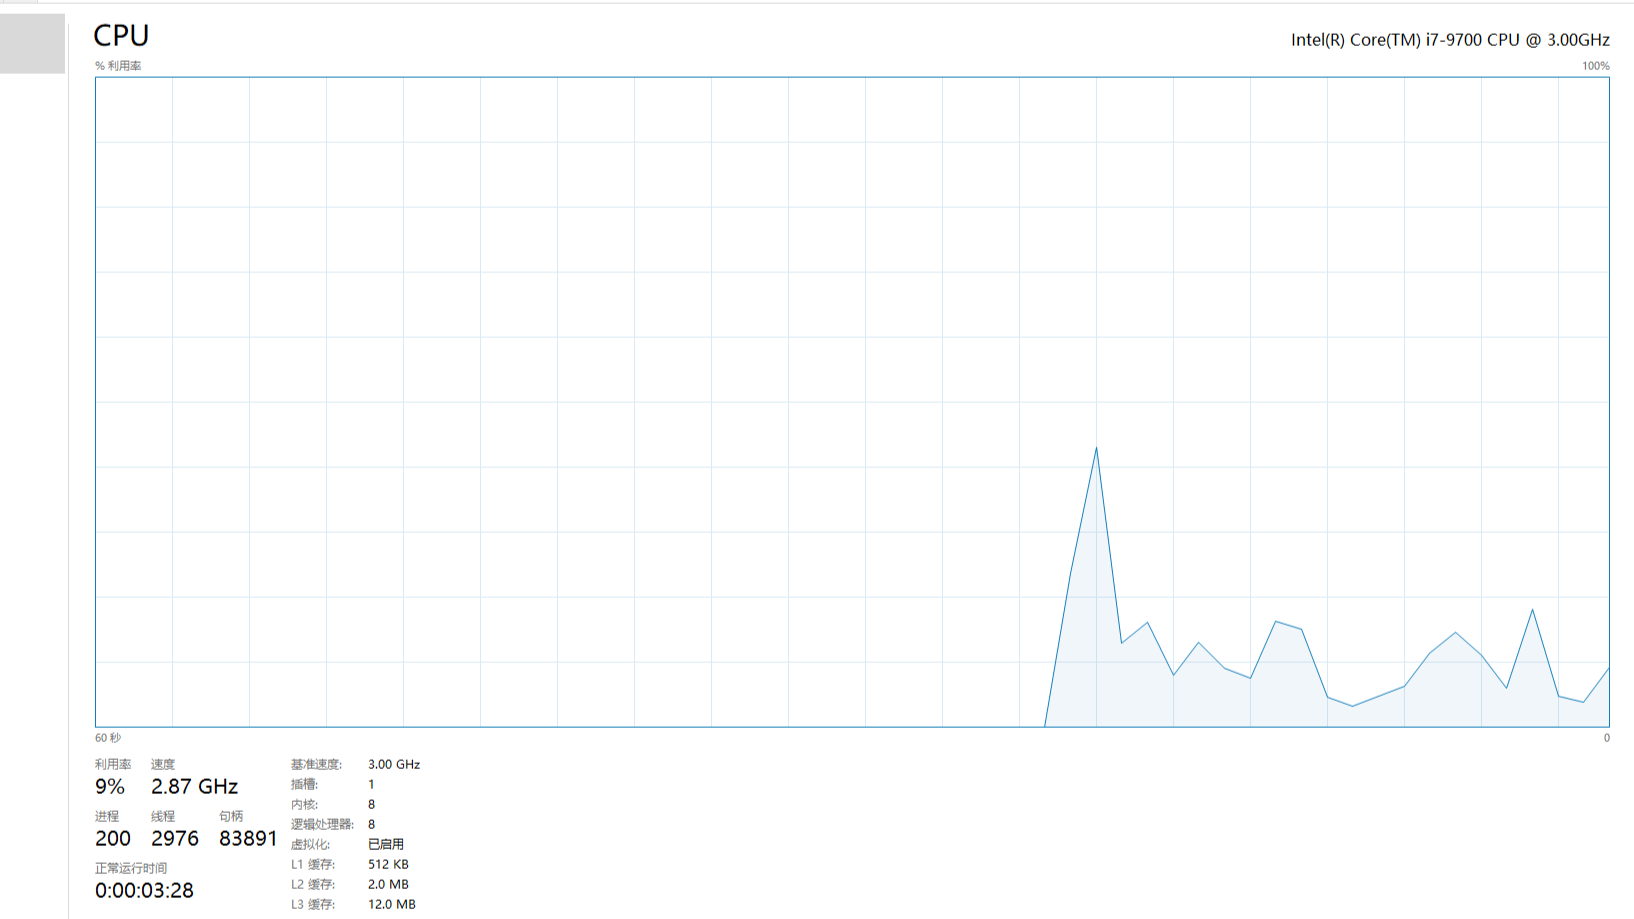
\includegraphics[width=1\textwidth]{figures/device_para/cpu.png}
		\caption{CPU参数}
		\label{fig:cpupara}
	\end{minipage}
	\begin{minipage}[t]{0.48\textwidth}
		\centering
		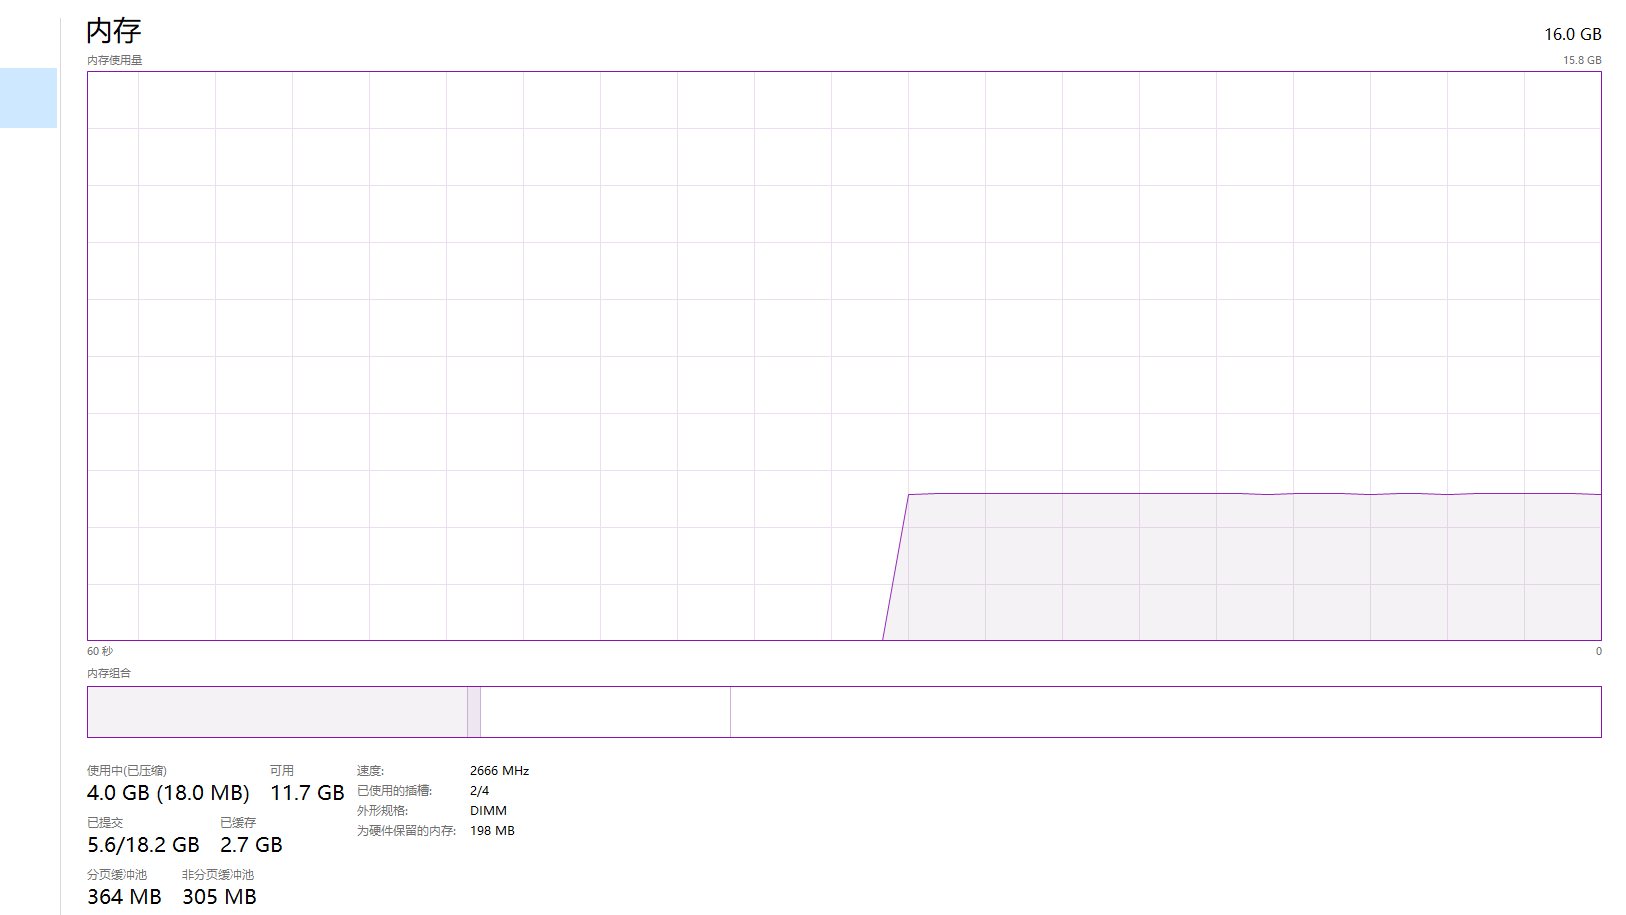
\includegraphics[width=1\textwidth]{figures/device_para/ram.png}
		\caption{RAM参数}
		\label{fig:rampara}
	\end{minipage}

	\centering
	\begin{minipage}[t]{0.48\textwidth}
		\centering
		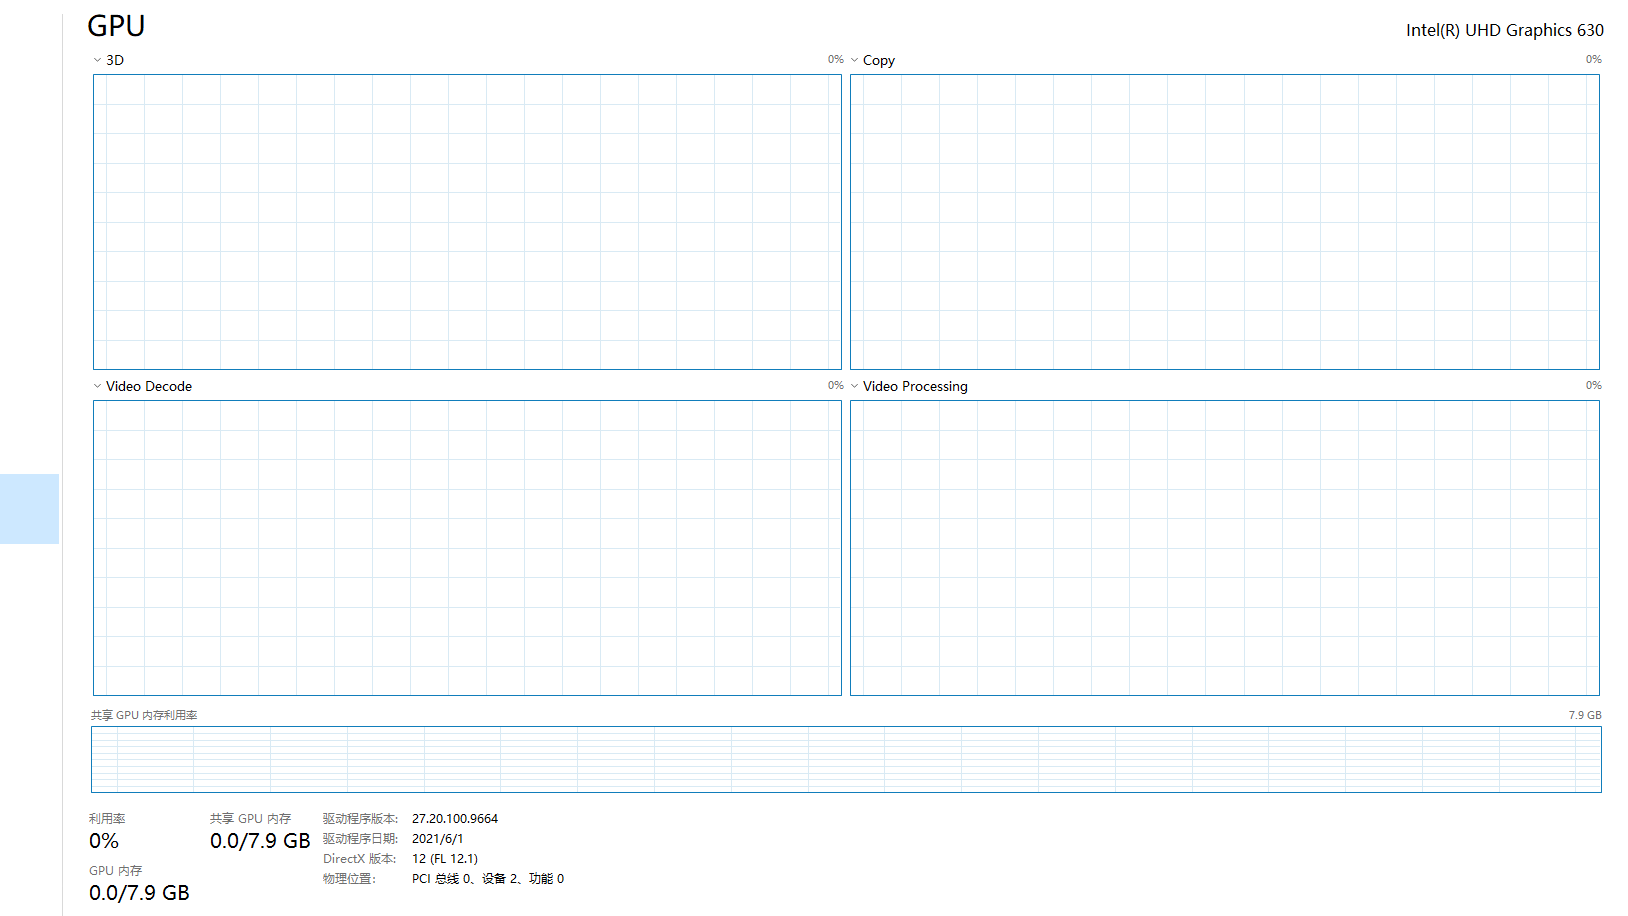
\includegraphics[width=1\textwidth]{figures/device_para/igp.png}
		\caption{IGP参数}
		\label{fig:igppara}
	\end{minipage}
	\begin{minipage}[t]{0.48\textwidth}
		\centering
		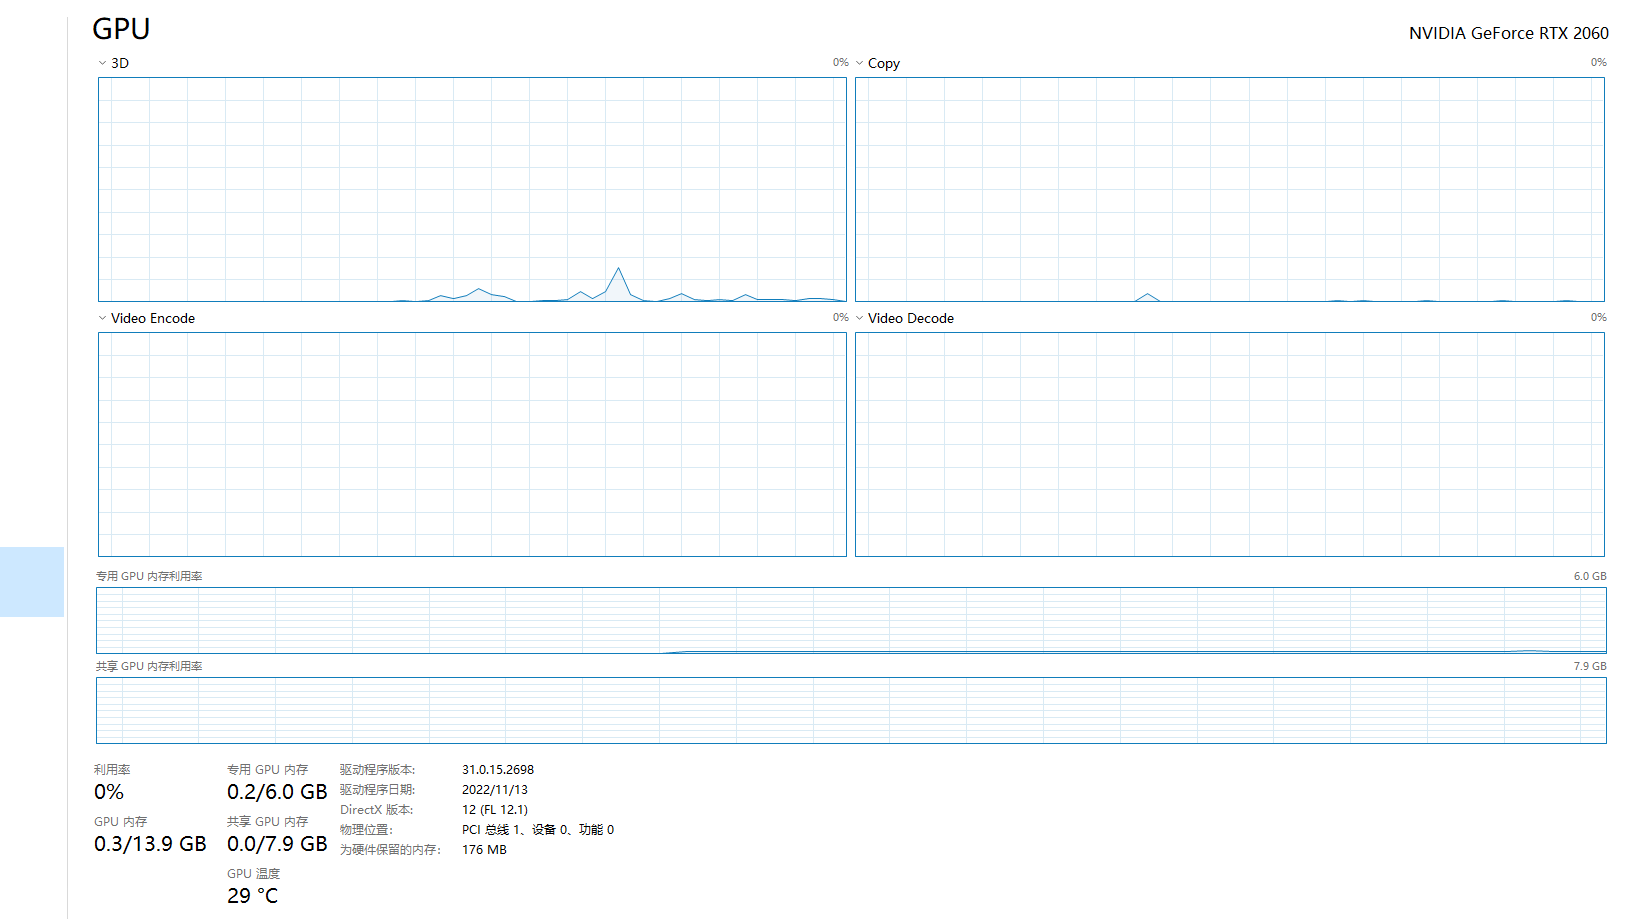
\includegraphics[width=1\textwidth]{figures/device_para/gpu.png}
		\caption{GPU参数}
		\label{fig:gpupara}
	\end{minipage}
\end{figure}

\begin{enumerate}
	\item{硬件环境}
	\par Intel Core i7-9700 CPU,16GB 内存(RAM),Intel(R) UHD Graphics 630集成图形处理器(IGP)和NVIDIA GeForce RTX 2060 GPU。所有计算均在此硬件环境上完成。
	具体信息见图\ref{fig:cpupara} $\sim$ 图\ref{fig:gpupara}。

	\item{操作系统}
	\par Windows 10 专业版 22H2 和 Ubuntu 20.04 LTS为主要的开发和运行环境,因其对开源软件和库支持良好。

	\item{开发语言}
	\par C++14和Python3.9。Python用于实现RGB图像语义分割,C++用于实现系统其他的所有功能。

	\item{开发工具}
	\par 使用Visual Studio Code 1.78和NVIDIA Nsight Compute 2022作为代码编辑器,CUDA 11.8进行GPU并行计算的开发,使用Git进行版本控制。

	\item{编译器}
	\par 使用GCC 11.3.0编译Ubuntu系统的C++代码,NVCC 11.7编译CUDA代码,以及MSVC 14.3编译Windows系统的C++代码。

	\item{依赖库}
	\par OpenCV 4.6用于图像处理,Open3D 0.16用于点云后处理,OpenGL 3.3和GLFW 3.3.8用于图形渲染和窗口管理,以及Intel Realsense SDK 2.0用于操作Intel Realsense相机。
\end{enumerate}

\section{详细设计}
\subsection{数据采集模块}
\par 该模块以\texttt{Frame}类(见表\ref{table:Frame})为主体,它统一管理RGB-D相机和图像数据,图像数据每帧更新一次,组件图和时序图如图\ref{fig:component1}、图\ref{fig:sequence1}所示。

% \begin{figure}[htb]
% 	\centering
% 	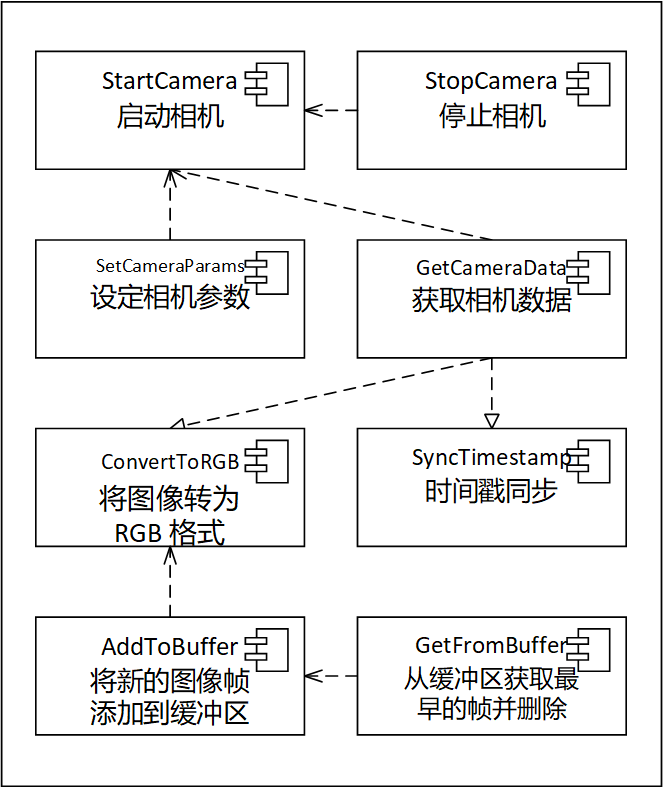
\includegraphics[width=0.7\textwidth]{figures/uml/component1.png}
% 	\caption{数据采集模块组件图}
% 	\label{fig:component1}
% \end{figure}

\begin{figure}[htb]
	\centering
	\begin{minipage}[t]{0.44\textwidth}
		\centering
		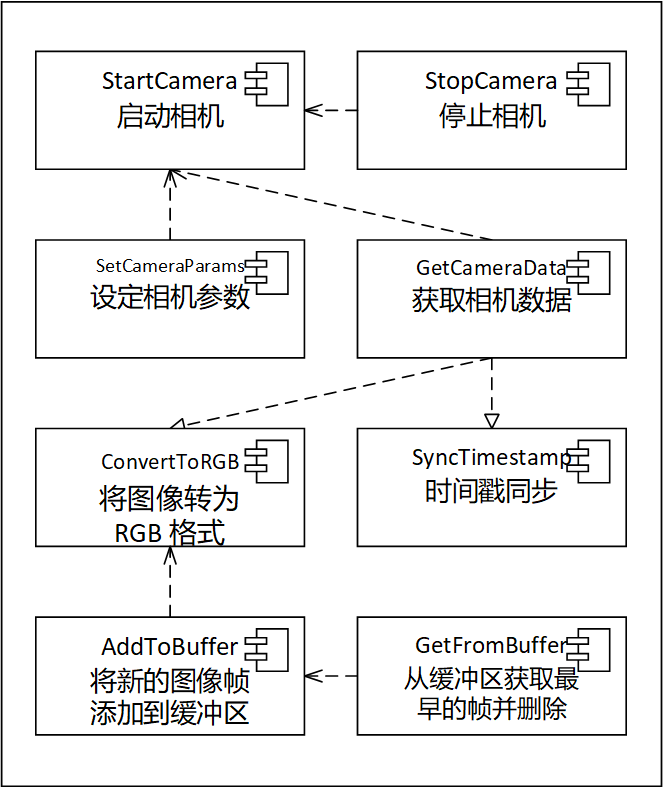
\includegraphics[height=7.5cm,keepaspectratio]{figures/uml/component1.png}
		\caption{数据采集模块组件图}
		\label{fig:component1}
	\end{minipage}
	\begin{minipage}[t]{0.51\textwidth}
		\centering
		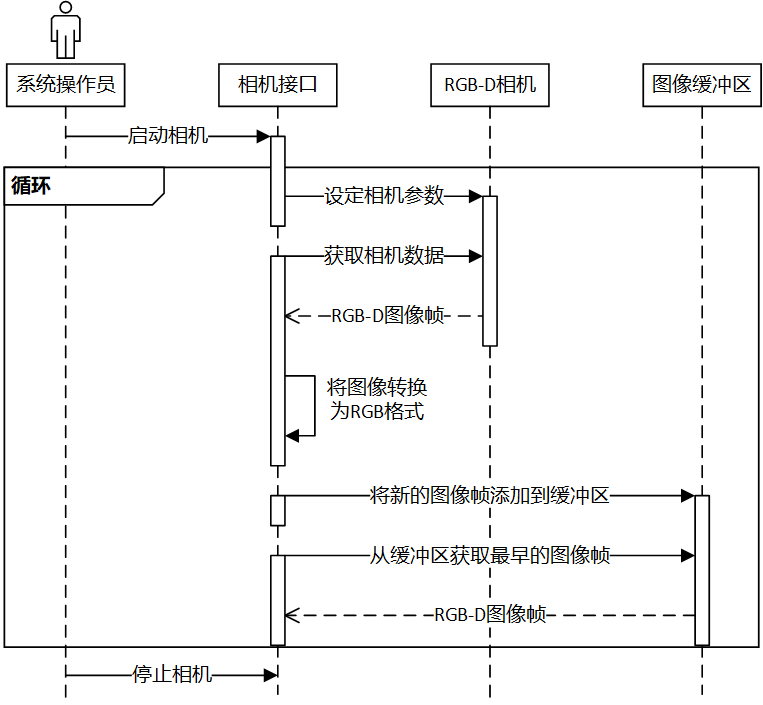
\includegraphics[height=7.5cm,keepaspectratio]{figures/uml/sequence1.png}
		\caption{数据采集模块时序图}
		\label{fig:sequence1}
	\end{minipage}
\end{figure}

\begin{table}[htb]
	\centering
	\caption{Frame类的主要成员和方法}
	\label{table:Frame}
	\begin{tabular}{|l|m{3.5cm}|m{3.5cm}|m{5cm}|}
		\hline
		                                           & \multicolumn{1}{c|}{名称}                         & \multicolumn{1}{c|}{类型}                       & \multicolumn{1}{c|}{功能}                 \\ \hline
		\multicolumn{1}{|c|}{\multirow{12}{*}{成员}} & \centering\arraybackslash current\_frame\_index & \centering\arraybackslash int                 & \centering\arraybackslash 当前帧的序号        \\ \cline{2-4}
		\multicolumn{1}{|c|}{}                     & \centering\arraybackslash pipeline              & \centering\arraybackslash rs2::pipeline       & \centering\arraybackslash RealSense相机对象 \\ \cline{2-4}
		\multicolumn{1}{|c|}{}                     & \centering\arraybackslash rgb\_width            & \centering\arraybackslash unsigned int        & \centering\arraybackslash RGB图像的宽度      \\ \cline{2-4}
		\multicolumn{1}{|c|}{}                     & \centering\arraybackslash rgb\_height           & \centering\arraybackslash unsigned int        & \centering\arraybackslash RGB图像的高度      \\ \cline{2-4}
		\multicolumn{1}{|c|}{}                     & \centering\arraybackslash depth\_width          & \centering\arraybackslash unsigned int        & \centering\arraybackslash 深度图像的宽度       \\ \cline{2-4}
		\multicolumn{1}{|c|}{}                     & \centering\arraybackslash depth\_height         & \centering\arraybackslash unsigned int        & \centering\arraybackslash 深度图像的高度       \\ \cline{2-4}
		\multicolumn{1}{|c|}{}                     & \centering\arraybackslash rgb\_image            & \centering\arraybackslash cv::Mat             & \centering\arraybackslash RGB图像         \\ \cline{2-4}
		\multicolumn{1}{|c|}{}                     & \centering\arraybackslash depth\_image          & \centering\arraybackslash cv::Mat             & \centering\arraybackslash 深度图像          \\ \cline{2-4}
		\multicolumn{1}{|c|}{}                     & \centering\arraybackslash semantic\_image       & \centering\arraybackslash cv::Mat             & \centering\arraybackslash 语义分割图像        \\ \cline{2-4}
		\multicolumn{1}{|c|}{}                     & \centering\arraybackslash rgb\_viewer           & \centering\arraybackslash Viewer              & \centering\arraybackslash RGB图像的位姿      \\ \cline{2-4}
		\multicolumn{1}{|c|}{}                     & \centering\arraybackslash depth\_viewer         & \centering\arraybackslash Viewer              & \centering\arraybackslash 深度图像的位姿       \\ \cline{2-4}
		\multicolumn{1}{|c|}{}                     & \centering\arraybackslash buffer                & \centering\arraybackslash queue          & \centering\arraybackslash 图像缓冲区         \\ \hline
		\multirow{14}{*}{方法}                       & \centering\arraybackslash StartCamera           & \centering\arraybackslash void                & \centering\arraybackslash 启动相机          \\ \cline{2-4}
		                                           & \centering\arraybackslash StopCamera            & \centering\arraybackslash void                & \centering\arraybackslash 停止相机          \\ \cline{2-4}
		                                           & \centering\arraybackslash SetCameraParams       & \centering\arraybackslash void                & \centering\arraybackslash 设定相机参数        \\ \cline{2-4}
		                                           & \centering\arraybackslash GetCameraData         & \centering\arraybackslash rs2::frameset       & \centering\arraybackslash 获取相机数据        \\ \cline{2-4}
		                                           & \centering\arraybackslash SyncTimestamp         & \centering\arraybackslash void                & \centering\arraybackslash 时间戳同步         \\ \cline{2-4}
		                                           & \centering\arraybackslash ConvertToRGB          & \centering\arraybackslash tuple          & \centering\arraybackslash 将图像转换为RGB格式   \\ \cline{2-4}
		                                           & \centering\arraybackslash AddToBuffer           & \centering\arraybackslash void                & \centering\arraybackslash 将新的图像帧添加到缓冲区  \\ \cline{2-4}
		                                           & \centering\arraybackslash GetFromBuffer         & \centering\arraybackslash tuple          & \centering\arraybackslash 从缓冲区获取最早的帧并删除 \\ \cline{2-4}
		                                           & \centering\arraybackslash AlignImage            & \centering\arraybackslash cv::Mat             & \centering\arraybackslash 对齐RGB图像和深度图像  \\ \cline{2-4}
		                                           & \centering\arraybackslash DenoiseImage          & \centering\arraybackslash cv::Mat             & \centering\arraybackslash 图像去噪与增强       \\ \cline{2-4}
		                                           & \centering\arraybackslash CropImage             & \centering\arraybackslash cv::Mat             & \centering\arraybackslash 裁剪图像的无效区域     \\ \cline{2-4}
		                                           & \centering\arraybackslash ResizeImage           & \centering\arraybackslash cv::Mat             & \centering\arraybackslash 图像缩放          \\ \cline{2-4}
		                                           & \centering\arraybackslash SegmentImage          & \centering\arraybackslash cv::Mat             & \centering\arraybackslash RGB图像语义分割     \\ \cline{2-4}
		                                           & \centering\arraybackslash NormalizeImage        & \centering\arraybackslash \_\_global\_\_ void & \centering\arraybackslash 图像格式转换和归一化    \\ \hline
	\end{tabular}
\end{table}

\par 首先,\texttt{StartCamera}通过调用Intel RealSense SDK 2.0的接口,启动Intel RealSense 相机。启动相机后,\texttt{SetCameraParams}设定相机的参数,包括图像分辨率、帧率、和深度距离。

\par 接下来,执行\texttt{GetCameraData}获取相机的数据。这个函数将返回一个包含RGB图像和深度图像的帧集。这里,通过调用\texttt{SyncTimestamp}确保RGB图像和深度图像的时间戳是同步的,它将根据相机型号,采用对应的硬件同步来对时间戳进行校正。

\par 获取和同步数据后,首先通过\texttt{ConvertToRGB}函数调用OpenCV接口,将图像转换成RGB格式。接着,通过\texttt{AddToBuffer}将图像添加到缓冲区,数据结构为\texttt{queue<tuple<cv::Mat, cv::Mat>>}。该函数首先检查当前缓冲区中存储的帧数是否达到了预设的上限。如果达到上限,将从缓冲区的前端(即最旧的帧)移除一帧数据。然后,将输入的RGB图像和深度图像包成一个元组,复制这些图像数据,再将该元组添加到缓冲区的末尾,即缓冲区的最新位置。

\par 相应地,\texttt{GetFromBuffer}的任务是从缓冲区获取最早的一帧数据。首先,它会检查缓冲区是否为空。如果缓冲区为空,那么它将抛出一个运行时错误,提示缓冲区无数据。如果缓冲区不为空,函数会从缓冲区的前端获取一个元组,并将其从缓冲区中删除。最后,返回该元组。

% \par 在数据采集模块中,数据流的控制以及异常处理与容错是非常重要的,这是通过\texttt{ControlDataFlow}函数来完成的。这个函数作为一个守护线程,负责协调数据采集和处理过程中的数据传递,确保数据的有效性、完整性和正确性。

\par 当数据采集的工作完成后,可以通过\texttt{StopCamera}函数停止相机。

\par 数据采集模块在整个系统中起着非常重要的角色。通过调用\texttt{Frame}类的部分函数,能够有效地管理和处理图像数据,为后续的任务提供高质量的数据输入。
\subsection{位姿估计与场景管理模块}
\par 该模块以\texttt{Viewer}类(见表\ref{table:Viewer})和\texttt{Space}类(见表\ref{table:Space})为主体,分别负责相机位姿的管理和场景空间点云数据的管理,组件图如图\ref{fig:component2}所示。
系统通过\texttt{ManageData}函数实现CPU与GPU之间的数据交换与管理。由于系统设计多线程编程,需要使用锁机制防止资源冲突,保证数据的同步和并发。

\begin{figure}[htb]
	\centering
	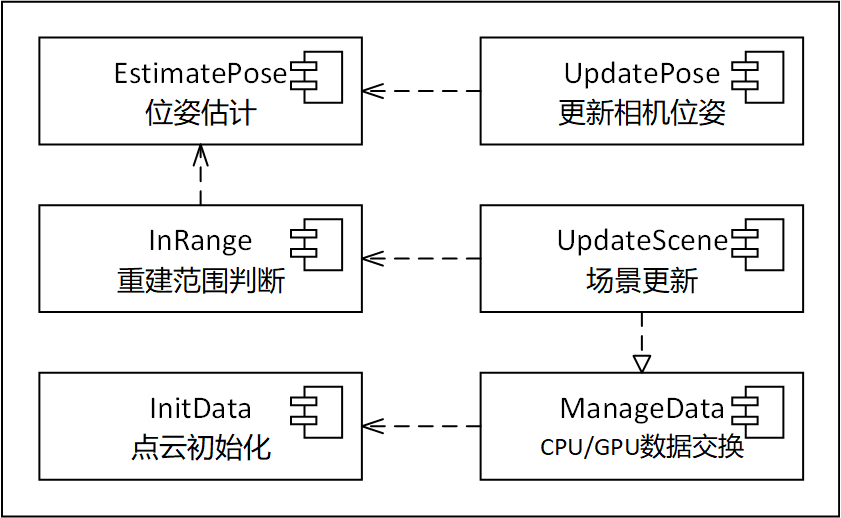
\includegraphics[width=0.7\textwidth]{figures/uml/component2.png}
	\caption{位姿估计与场景管理模块组件图}
	\label{fig:component2}
\end{figure}

\par 首先,位姿估计的任务由\texttt{Viewer}类的成员函数\texttt{EstimatePose}完成。当数据采集模块获得一帧新
的RGB-D数据,即\texttt{curr\_frame}后,利用对极几何原理,根据前一帧数据\texttt{old\_frame}
与\texttt{curr\_frame}之间的连续性和一致性,计算出当前相机的位姿矩阵并转换为一维数组存储到\texttt{pose}中:
\begin{align}
	T_{cam} & =
	\begin{bmatrix}
		R   & t \\
		0^T & 1
	\end{bmatrix}
	=
	\begin{bmatrix}
		\texttt{pose[0]}  & \texttt{pose[1]}  & \texttt{pose[2]}  & \texttt{pose[3]}  \\
		\texttt{pose[4]}  & \texttt{pose[5]}  & \texttt{pose[6]}  & \texttt{pose[7]}  \\
		\texttt{pose[8]}  & \texttt{pose[9]}  & \texttt{pose[10]} & \texttt{pose[11]} \\
		\texttt{pose[12]} & \texttt{pose[13]} & \texttt{pose[14]} & \texttt{pose[15]}
	\end{bmatrix}
\end{align}

\par 其中,$R$是 $3 \times 3$ 的旋转矩阵,$t$是 $3 \times 1$ 的平移向量。因此,对于相机坐标系中的点$P_{cam}$,可以通过公式\ref{pose_matrix}
计算出其在世界坐标系中对应的坐标 $P_w$:
\begin{equation*}
	\text{令}P_w =
	\begin{bmatrix}
		x_w \\
		y_w \\
		z_w
	\end{bmatrix}\text{,}
	P_{cam} =
	\begin{bmatrix}
		x_{cam} \\
		y_{cam} \\
		z_{cam}
	\end{bmatrix}
\end{equation*}

\par 于是,相机坐标系到世界坐标系的转换为:

\begin{equation}
	\begin{bmatrix}
		P_w \\
		1
	\end{bmatrix}
	= T_{cam}
	\begin{bmatrix}
		P_{cam} \\
		1
	\end{bmatrix}
	=
	\begin{bmatrix}
		R   & t \\
		0^T & 1
	\end{bmatrix}
	\begin{bmatrix}
		P_{cam} \\
		1
	\end{bmatrix}
	=
	\begin{bmatrix}
		RP_{cam} + t \\
		1
	\end{bmatrix}
	\label{pose_matrix}
\end{equation}

\par 位姿矩阵将为后续的三维重建提供基本的空间信息。一旦计算出位姿矩阵,就可以通过\texttt{UpdatePose}将相机位置和朝向信息更新到\texttt{Viewer}类中,供可视化模块使用。

\begin{table}[htb]
	\centering
	\caption{Viewer类的主要成员和方法}
	\label{table:Viewer}
	\begin{tabular}{|l|m{4cm}|m{3cm}|m{5cm}|}
		\hline
		                    & \multicolumn{1}{c|}{名称}                   & \multicolumn{1}{c|}{类型}          & \multicolumn{1}{c|}{功能}                         \\ \hline
		\multirow{7}{*}{成员} & \centering\arraybackslash intrinsic       & \centering\arraybackslash Matrix & \centering\arraybackslash 相机内参                  \\ \cline{2-4}
		                    & \centering\arraybackslash pose            & \centering\arraybackslash Matrix & \centering\arraybackslash 当前相机的位姿               \\ \cline{2-4}
		                    & \centering\arraybackslash position{[}3{]} & \centering\arraybackslash float  & \centering\arraybackslash \multirow{3}{*}{相机朝向} \\ \cline{2-3}
		                    & \centering\arraybackslash front{[}3{]}    & \centering\arraybackslash float  & \centering\arraybackslash                       \\ \cline{2-3}
		                    & \centering\arraybackslash gaze{[}3{]}     & \centering\arraybackslash float  & \centering\arraybackslash                       \\ \cline{2-4}
		                    & \centering\arraybackslash curr\_frame     & \centering\arraybackslash Frame  & \centering\arraybackslash 当前帧                   \\ \cline{2-4}
		                    & \centering\arraybackslash old\_frame      & \centering\arraybackslash Frame  & \centering\arraybackslash 上一帧                   \\ \hline
		\multirow{2}{*}{方法} & \centering\arraybackslash EstimatePose    & \centering\arraybackslash void   & \centering\arraybackslash 位姿估计                  \\ \cline{2-4}
		                    & \centering\arraybackslash UpdatePose      & \centering\arraybackslash void   & \centering\arraybackslash 更新相机位置和朝向             \\ \hline
	\end{tabular}
\end{table}

\par 在获得第一帧图像之前,模块首先实例化一个\texttt{Space}对象来管理场景空间和点云数据。系统先调
用\texttt{InitData}函数初始化点云数据,设定空间的原点坐标,设置场景重建的范围和点之间的距离,以
及\texttt{Point}结构体类型(见表\ref{table:point})的点云数组,包含每个点的坐标、RGB、类别标签等信息。

\begin{table}[htb]
	\centering
	\caption{Point结构体的成员}
	\begin{tabular}{cm{2.2cm}m{2.2cm}m{2.2cm}m{2.2cm}m{2.2cm}}
		\toprule
		名称 & \centering\arraybackslash x        & \centering\arraybackslash y     & \centering\arraybackslash z            & \centering\arraybackslash color\_b & \centering\arraybackslash color\_g      \\
		类型 & \centering\arraybackslash float    & \centering\arraybackslash float & \centering\arraybackslash float        & \centering\arraybackslash float    & \centering\arraybackslash float         \\
		\midrule
		名称 & \centering\arraybackslash color\_r & \centering\arraybackslash tsdf  & \centering\arraybackslash tsdf\_weight & \centering\arraybackslash label    & \centering\arraybackslash label\_weight \\
		类型 & \centering\arraybackslash float    & \centering\arraybackslash float & \centering\arraybackslash float        & \centering\arraybackslash int      & \centering\arraybackslash float         \\
		\bottomrule
	\end{tabular}
	\label{table:point}
\end{table}

\par 在场景管理过程中,系统在逻辑上将三维空间划分为四分之一重叠空间网格。\texttt{EstimatePose}计算出每一帧的
位姿矩阵后,首先调用\texttt{InRange}确定新的图像中的重建空间是否在当前的网格内,该
函数根据当前相机位姿进行判断。如果新的重建空间在当前的网格内,则进入点云生成与语义融合操作;如
果超出了范围,则需要进行场景更新。

\par 场景更新通过调用\texttt{UpdateScene}函数实现。首先,该函数调用\texttt{ManageData},将GPU中的点云数据
拷贝回CPU的点云数组中,调用模型导入导出模块,根据坐标所在的网格位置将点云模型保存为数据
文件。然后根据相机的位姿和相机内参,确定新的重建空间所在的网格,根据网格序号找到对应的数据
文件并导入。保存或加载模型时,需要指定场景序号,以方便后续的索引和查询。具体网格划分方法如
下:

\begin{figure}[htb]
	\centering
	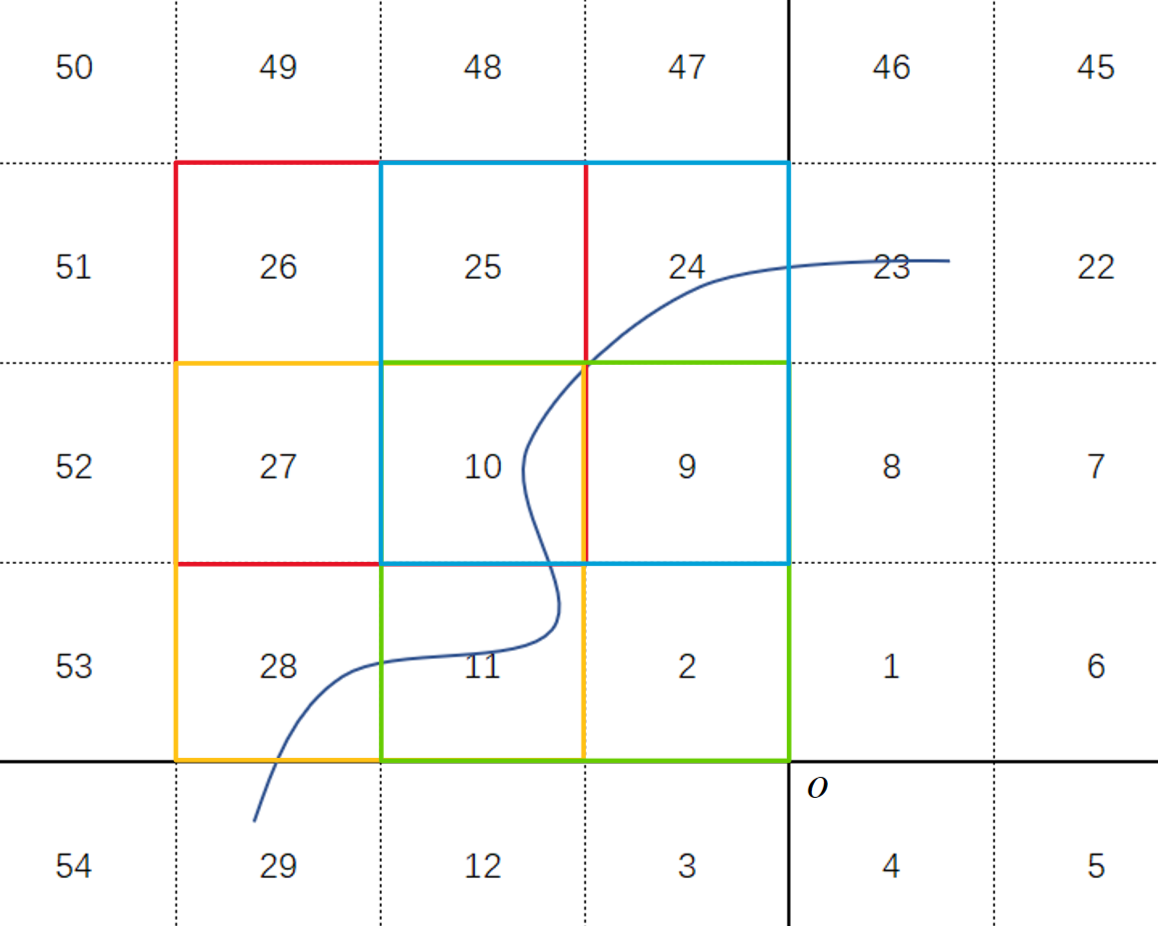
\includegraphics[width=0.7\textwidth]{figures/spatial_grid.png}
	\caption{网格划分方法}
	\note{注:在三维空间中采用逆时针螺旋方式进行网格划分的过程,通过实时更新相机位姿信息,处理四个相邻的网格以避免丢失重建空间。}
	\label{fig:spatial_grid}
\end{figure}

\par 在图\ref{fig:spatial_grid}中的原点处开始划分三维空间的网格。每个网格的序号按
逆时针螺旋形方式分配,与原点距离越近的网格序号越小。为了避免相机在运动过程中丢失重建空间,
系统在任何时刻都可以处理4个相邻的网格。图中,这四个网格被分
别标记为红色、蓝色、橙色和绿色区域。系统利用相机的实时位姿信息来确定每一帧图像的重建区域。
假设相机从29号网格开始向右上方移动,其在空间中的位置依次经过以(-2, 1), (-1, 1)和(-1, 2)为中心的网格。根据这些坐标点的位置,
可以确定系统当前需要处理的网格分别位于橙色、绿色和蓝色的区域。

\par 该网格划分方法大幅度减少了场景更新次数,从而提高了整个系统的运行效率。例如,在自动
驾驶系统中,如果汽车的速度为 12.5 m/s,每个网格的边长为 40 m,帧率为 30 帧/秒,那么在最快的情
况下,系统只需要每96帧(即每 3.2 秒)进行一次场景更新。

\par 该模块通过上述过程,在保证实时性和准确性的同时,实现了空间的有效划
分和数据的高效管理。通过位姿估计,可以获得相机的空间位置和朝向,从而定位场景和生成点云;
通过场景管理,可以进行动态场景重建,将重建范围扩大至无穷。
\subsection{数据预处理与语义分割模块}
\par 该模块利用\texttt{Frame}类对每一帧图像进行统一管理,包括RGB图像、深度图像以及语义分割图像,组件图如图\ref{fig:component3}所示。

\par 当新一帧的数据通过数据采集模块获取后,首先对RGB图像和深度图像进行对齐。对齐的过程是
通过调用\texttt{AlignImage}实现的,它使用Intel RealSense相机内参以及RGB图像和深度图像的位姿矩阵
进行校准,从而确保了在后续的三维重建过程中,RGB像素点和对应深度像素点的时间戳是相同的。

\begin{figure}[htbp]
	\centering
	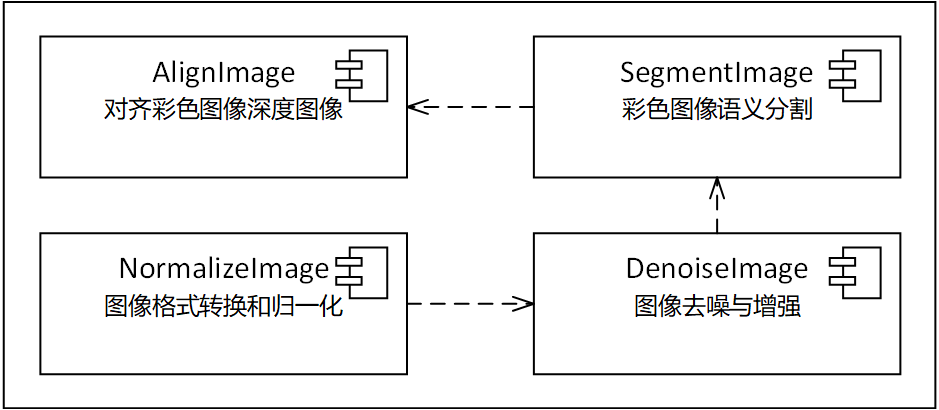
\includegraphics[width=0.7\textwidth]{figures/uml/component3.png}
	\caption{数据预处理与语义分割模块组件图}
	\label{fig:component3}
\end{figure}

\par 接着,系统将对RGB图像进行语义分割。这一步由\texttt{SegmentImage}完成,该函数会加载预训练的
“kMaX-DeepLab with ConvNeXt-large backbone with output stride 32” SavedModel模型进行推理,
为每个像素赋予一个类别标签。有了这些标签,系统就可以根据这些信息提高后续三维重建的精度和准确性。

% \begin{algorithm}[htb]
% 	\SetAlgoLined
% 	\KwData{RGB图像 rgb\_image, 模型路径 model\_path}
% 	\KwResult{语义分割图像 segmented\_image}
% 	% $\textit{session} \gets \text{TensorFlow.NewSession()}$\hspace{0.5cm}\tcp{创建一个新的TensorFlow会话}

% 	\tcp{创建一个新的TensorFlow会话}
% 	$\textit{session} \gets \text{TensorFlow.NewSession()}$\;

% 	\tcp{加载给定路径的模型}
% 	$\textit{graph\_def} \gets \text{TensorFlow.LoadModel}(\textit{model\_path})$\;

% 	\tcp{在会话中创建模型的图定义}
% 	$\textit{session.Create}(\textit{graph\_def})$\;

% 	\tcp{从RGB图像创建一个张量}
% 	$\textit{image\_tensor} \gets \text{CreateTensorFromImage}(\textit{rgb\_image})$\;

% 	\tcp{在会话中运行图像张量并获取输出}
% 	$\textit{outputs} \gets \text{session.Run}(\textit{image\_tensor})$\;

% 	\tcp{将输出结果转换为Mat类型的分割图像}
% 	$\textit{segmented\_image} \gets \text{ConvertOutputToMat}(\textit{outputs})$\;

% 	\caption{SegmentImage}
% 	\label{algo:SegmentImage}
% \end{algorithm}

\par 对图像进行语义分割之后,需要进行去噪与增强。\texttt{DenoiseImage}调用OpenCV的中值滤波函数接口 \texttt{cv::medianBlur}
和高斯滤波函数接口 \texttt{cv::GaussianBlur},去除图像中的脉冲噪声和高斯噪声。然后根据相机的视场、测量范围和深度信息,对图像进行裁剪,去除图像中的无效区域。接着,将RGB图像和语义分割图像缩放至$1296 \times 968$,将深度图像缩放至$640 \times 480$。

\begin{algorithm}[htbp]
	\SetAlgoLined
	\KwData{原始图像数据 src, 像素数组 des, 图像类型 type, 每行字节数 step}
	\KwResult{归一化图像数据}
	用块和线程索引初始化整数变量 $c$, $r$, $channel$, $w$, $h$\;
	\If{当前图像为RGB图像}{
		计算目标索引 $i = (r * w + c) * 3 + channel$\;
		使用 $v = int(src[r * step + c * 3 + channel])$ 从图像中获取像素值\;
		使用 $v = v / 255.0f$ 归一化值\;
		使用 $des[i] = v$ 将像素值赋给目标数组\;
	}
	\ElseIf{当前图像为深度图像}{
		初始化ushort变量 $depth\_us = 0$\;
		用 $depth\_us = depth\_us | src[r * step + c * 2 + 1]$ 更新 $depth\_us$\;
		改变字节序列 $depth\_us = depth\_us << 8$\;
		用 $depth\_us = depth\_us | src[r * step + c * 2]$ 更新 $depth\_us$\;
		使用 $depth\_val = (float)(depth\_us) / 1000.0f$ 归一化深度值\;
		如果深度值大于 6.0f,则设为 0.0f\;
		使用 $des[r * w + c] = depth\_val$ 将深度值赋给目标数组\;
	}
	\Else{
		计算目标索引 $i = (r * w + c) * 3 + channel$\;
		使用 $v = int(src[r * step + c * 3 + channel])$ 从图像中获取像素值\;
		如果通道是 2,使用 $v = v / 255.0f$ 归一化值\;
		使用 $des[i] = v$ 将值赋给目标数组\;
	}
	\caption{NormalizeImage}
	\label{algo:NormalizeImage}
\end{algorithm}

\par 最后,进行图像的格式转换和数值归一化。通过调用CUDA环境下运行的一个\texttt{\_\_global\_\_}函数
\texttt{NormalizeImage}实现,伪代码如算法\ref{algo:NormalizeImage}所示。输入参数中,\texttt{src}是原始图像数据,\texttt{des}是存放输出结果的像素数组,\texttt{type}用
于区分图像类型,\texttt{step}是图像中每行的字节数。该函数在CUDA内核中执行,利用
并行计算加速图像处理过程。该函数将图像的格式转换成系统规定的格式,并将每个像素的值归一化,
使得它们在0到1之间:

\par 首先,函数根据CUDA线程模型中的\texttt{blockIdx}和\texttt{threadIdx}来计算在图像中处理的具体位置。具
体地,\text{c}和\text{r}是图像的列和行,而\text{channel}是处理的RGB通道。然后,根据\texttt{type}的值来确定图像类型。如
果\texttt{type}是0或2,表示这是一个RGB图像或语义分割图像。函数将像素值从整型[0, 255]转换为浮点型[0.0, 1.0],并按
照$\text{index} = (\text{r} \times \text{w} + \text{c}) \times 3 + \text{channel}$的方式存储到\texttt{des}中。如果\texttt{type}是1,表示这是一个深度图像。由于
深度图像中的每个像素值存储为2 byte的ushort类型,且设备大小端存在冲突,因此需要特殊处理。
函数先读取两个连续的uchar(每个uchar占1字节),然后通过位运算和大小端转换将这两个uchar拼
接成一个ushort。最后,将ushort类型的深度值转换为浮点型并除以1000.0f,得到单位为米的深度值。
如果深度值大于6.0m,则将其设置为0.0,然后按照$\text{index} = \text{r} \times \text{w} + \text{c}$的方式存储到\texttt{des}中。
\subsection{点云生成与语义融合模块}
\par 该模块以\texttt{Space}类为主体,使用GPU资源进行实时计算,生成并更新包含RGB信息和语义信息的三维模型。\texttt{Space}类与其他类的关系见图\ref{fig:class4}。模块通过 TSDF 算法生成点云,使用线性分配方法将语义分割信息融入每一个点云中。

\begin{table}[htb]
	\centering
	\caption{Space类的主要成员和方法}
	\label{table:Space}
	\begin{tabular}{|l|m{2.8cm}|m{4.7cm}|m{4.5cm}|}
		\hline
		                     & \multicolumn{1}{c|}{名称}                  & \multicolumn{1}{c|}{类型}                                & \multicolumn{1}{c|}{功能}                         \\ \hline
		\multirow{11}{*}{成员} & \centering\arraybackslash k\_origin\_x   & \centering\arraybackslash const float                  & \centering\arraybackslash \multirow{3}{*}{原点坐标} \\ \cline{2-3}
		                     & \centering\arraybackslash k\_origin\_y   & \centering\arraybackslash const float                  & \centering\arraybackslash                       \\ \cline{2-3}
		                     & \centering\arraybackslash k\_origin\_z   & \centering\arraybackslash const float                  & \centering\arraybackslash                       \\ \cline{2-4}
		                     & \centering\arraybackslash k\_space\_x    & \centering\arraybackslash const float                  & \centering\arraybackslash \multirow{3}{*}{重建范围} \\ \cline{2-3}
		                     & \centering\arraybackslash k\_space\_y    & \centering\arraybackslash const float                  & \centering\arraybackslash                       \\ \cline{2-3}
		                     & \centering\arraybackslash k\_space\_z    & \centering\arraybackslash const float                  & \centering\arraybackslash                       \\ \cline{2-4}
		                     & \centering\arraybackslash k\_point\_size & \centering\arraybackslash const float                  & \centering\arraybackslash 点云分辨率(单位:米)           \\ \cline{2-4}
		                     & \centering\arraybackslash point\_num     & \centering\arraybackslash unsigned int                 & \centering\arraybackslash 点的数量                  \\ \cline{2-4}
		                     & \centering\arraybackslash trunc\_margin  & \centering\arraybackslash float                        & \centering\arraybackslash 截断边界                  \\ \cline{2-4}
		                     & \centering\arraybackslash point\_list    & \centering\arraybackslash Point                        & \centering\arraybackslash 点云结构体数组               \\ \cline{2-4}
		                     & \centering\arraybackslash pcd            & \centering\arraybackslash open3d.geometry.PointCloud   & \centering\arraybackslash Open3D点云对象            \\ \hline
		\multirow{14}{*}{方法} & \centering\arraybackslash InitData       & \centering\arraybackslash void                         & \centering\arraybackslash 点云数据初始化               \\ \cline{2-4}
		                     & \centering\arraybackslash SaveCloud      & \centering\arraybackslash void                         & \centering\arraybackslash 点云模型存储                \\ \cline{2-4}
		                     & \centering\arraybackslash LoadCloud      & \centering\arraybackslash void                         & \centering\arraybackslash 点云模型加载                \\ \cline{2-4}
		                     & \centering\arraybackslash InRange        & \centering\arraybackslash bool                         & \centering\arraybackslash 重建范围判断                \\ \cline{2-4}
		                     & \centering\arraybackslash UpdateScene    & \centering\arraybackslash \_\_global\_\_ void          & \centering\arraybackslash 场景更新                  \\ \cline{2-4}
		                     & \centering\arraybackslash ManageData     & \centering\arraybackslash \_\_host\_\_ void            & \centering\arraybackslash CPU / GPU 数据交换与管理     \\ \cline{2-4}
		                     & \centering\arraybackslash Construct      & \centering\arraybackslash \_\_global\_\_ void          & \centering\arraybackslash 点云生成及语义融合             \\ \cline{2-4}
		                     & \centering\arraybackslash GetNeighbour   & \centering\arraybackslash \_\_device\_\_ vector        & \centering\arraybackslash 获取邻域点的信息              \\ \cline{2-4}
		                     & \centering\arraybackslash DenoiseRGB     & \centering\arraybackslash \_\_device\_\_ void          & \centering\arraybackslash RGB信息滤波               \\ \cline{2-4}
		                     & \centering\arraybackslash DenoiseLabel   & \centering\arraybackslash \_\_device\_\_ void          & \centering\arraybackslash 类别标签滤波                \\ \cline{2-4}
		                     & \centering\arraybackslash ToOpen3DPoint  & \centering\arraybackslash void                         & \centering\arraybackslash Open3D格式转换            \\ \cline{2-4}
		                     & \centering\arraybackslash Downsample     & \centering\arraybackslash void                         & \centering\arraybackslash 八叉树下采样                \\ \cline{2-4}
		                     & \centering\arraybackslash EstimateNormal & \centering\arraybackslash open3d.geometry.PointCloud   & \centering\arraybackslash PCA法线估计               \\ \cline{2-4}
		                     & \centering\arraybackslash GreedyProjTri  & \centering\arraybackslash open3d.geometry.TriangleMesh & \centering\arraybackslash 贪婪投影三角化               \\ \hline
	\end{tabular}
\end{table}

\begin{figure}[htb]
	\centering
	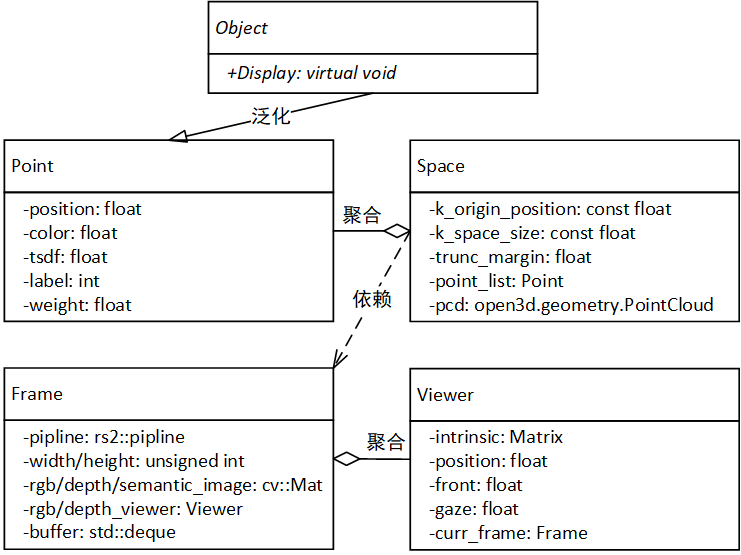
\includegraphics[width=0.7\textwidth]{figures/uml/class4.png}
	\caption{点云生成与语义融合模块类图}
	\label{fig:class4}
\end{figure}

\par 在获取数据预处理与语义分割模块传递来的数据后,通过\texttt{ManageData}函数将CPU中的数据拷贝到GPU内存中。随后,调用\texttt{Construct}进行实时点云的生成,语义融合与更新。\texttt{Construct}输入的参数包括\texttt{Point}类型的点云数组、RGB图像、深度图像、语义分割图像以及内参矩阵和相机位姿。
与\texttt{NormalizeImage}相同,\texttt{Construct}也是一个\texttt{\_\_global\_\_}函数,全部过程运行在GPU上,具体流程如下:

\begin{enumerate}
	\item 根据CUDA线程模型中的\texttt{blockIdx}和\texttt{threadIdx}计算线程序号,并根据这个序号计算当前线程需要处理的点在世界坐标系下的坐标(x, y, z)。

	\item 通过该点的全局三维坐标$P_w$和提供的相机内参、相机位姿,计算出相机坐标$P_{cam}$。根据公式\ref{pose_matrix}可知:
	      \begin{equation}
		      P_{cam} = R^T(P_w - t)
	      \end{equation}

	      因此,可以根据\texttt{pose}计算出该点的相机坐标:
	      \begin{equation}
		      \begin{aligned}
			      x_{cam} = & \texttt{pose[0]} \times (x_w - \texttt{pose[3]}) + \texttt{pose[4]} \times (y_w - \texttt{pose[7]}) \\
			                & + \texttt{pose[8]} \times (z_w - \texttt{pose[11]})                                                 \\
			      y_{cam} = & \texttt{pose[1]} \times (x_w - \texttt{pose[3]}) + \texttt{pose[5]} \times (y_w - \texttt{pose[7]}) \\
			                & + \texttt{pose[9]} \times (z_w - \texttt{pose[11]})                                                 \\
			      z_{cam} = & \texttt{pose[2]} \times (x_w - \texttt{pose[3]}) + \texttt{pose[6]} \times (y_w - \texttt{pose[7]}) \\
			                & + \texttt{pose[10]} \times (z_w - \texttt{pose[11]})
		      \end{aligned}
		      \label{cam_coordinates}
	      \end{equation}

	      计算出相机坐标后,检查该点是否位于相机前方且在预定距离内。如果不在则直接返回,结束当前线程的执行。

	\item 若当前点满足相机视野的条件,则对点进行投影变换,使用相机内参矩阵将其坐标从相机坐标系转换为图像坐标系,即计算出该点在图像中的像素坐标 $P_{pix}$ :
	      \begin{equation}
		      \begin{aligned}
			      x_{pix} = \texttt{intrinsic[0]} \times \frac{x_{cam}}{z_{cam}} + \texttt{intrinsic[2]} \\
			      y_{pix} = \texttt{intrinsic[4]} \times \frac{y_{cam}}{z_{cam}} + \texttt{intrinsic[5]}
		      \end{aligned}
	      \end{equation}

	      然后,判断转换后的像素坐标是否在图像范围内,如果不在则直接返回。

	\item 对于满足以上条件的点,计算其在RGB图像、深度图像和语义分割图像中的位置,并读取对应位置的RGB值、深度值和类别标签,对深度值进行检查,如果值过小或过大,则直接返回。

	\item 点云生成,计算点的TSDF值。TSDF值即点相对于观测到的表面的距离,通过该点在相机视野中的深度和真实深度之间的差值来计算。如果计算得到的TSDF值小于截断范围的负值,则直接返回。否则,在1.0f和自身与截断范围的比值之间取较小值,使用一个权重系统与旧的TSDF值进行加权平均更新TSDF值,以处理多个视角的影响,公式如下:
	      \begin{equation}
		      TSDF_{i} = \frac{TSDF_{i-1} \times W_{i-1} + tsdf_{i} \times w_{i}}{W_{i-1} + w_{i}}
	      \end{equation}

	      \par 这里的 $TSDF_{i-1}$ 和 $W_{i-1}$ 即当前点存储的前 $i-1$ 次更新的 TSDF 值和权重,$tsdf_{i}$ 是根据当前深度图计算出来的第$i$帧的 TSDF 值,$w_{i}$ 是当前更新的权重。

	\item 实时语义融合与更新。这里采取与 Panopticfusion相似的方法,在每次将某个点匹配到目标类别标签以及置信度后,使用线性分配的方式更新类别标签\cite{panopticfusion,VolumetricMethod},具体方法如下:

	      \par 对于每个时间步长$t$和体素$v$,根据公式
	      \begin{equation}
		      W(t, v)=\left\{\begin{array}{ll}
			      W(t-1, v)+w(t, v) & l_{d}(t, v)=l_{\tau}(t, v)                                    \\
			      W(t-1, v)-w(t, v) & l_{d}(t, v) \neq l_{\tau}(t, v) \wedge W(t-1, v) \geq w(t, v) \\
			      w_{t}(v, d)       & l_{d}(t, v) \neq l_{\tau}(t, v) \wedge W(t-1, v)<w(t, v)
		      \end{array}\right.
		      \label{equ:lap}
	      \end{equation}

	      计算权重 $W(t, v)$,其中 $l_{\tau}(t, v) \in L$ 和 $w(t, v)$ 是当前点在前图像帧中关联的目标类别标签的全局序号和置信度,$l_{d}(t, v) \in L$ 和 $W(t-1, v)$ 是当前点在先前图像帧中已经关联的目标类别标签的全局序号和置信度,即\texttt{label}和\texttt{label\_weight}。
	      如果在当前图像帧中该点的置信度显著减小,例如当 $l_{d}(t, v) \neq l_{\tau}(t, v) \land W(t - 1, v) < w(t, v)$ 时,会重置该点的全局序号为 $l_{d}(t, v)$,如公式\ref{equ:lap}中的最后一种情况所示。这样,每个点只需要存储一个类别标签的全局序号,而不需要记录每个点关联的所有类别标签。

	      \begin{algorithm}[htbp]
		      \SetAlgoLined
		      \KwData{点云结构体数组 point\_list, RGB图像 rgb\_image, 深度图像 depth\_image, 语义分割图像 semantic\_image, 相机内参 intrinsic, 相机位姿(外参) pose}
		      \KwResult{更新后的包含语义信息的点云}
		      \ForEach{thread in GPU}{
			      使用blockIdx和threadIdx计算线程索引\;
			      根据线程索引从 $point_list$ 获取当前点 $p$\;
			      根据 $intrinsic$、$intrinsic$ 计算当前点的相机系坐标\;
			      \If{$p$ 不在相机前方或不在预设距离内}{
				      继续\;
			      }
			      使用 $intrinsic$ 将 $p$ 的相机系坐标 $p_{c}$ 转换为图像系坐标 $p_{i}$\;
			      \If{$p_{i}$ 不在图像范围内}{
				      继续\;
			      }
			      将 $p$ 投影到 $rgb\_image$、$depth\_image$ 和 $semantic\_image$\;
			      获取 $p$ 相应的RGB值、深度值和类别标签\;
			      \If{深度值不在合理范围内}{
				      继续\;
			      }
			      为 $p$ 计算TSDF值\;
			      \If{TSDF值小于截断范围的负值}{
				      继续\;
			      }
			      使用加权平均方法更新TSDF值\;
			      使用线性分配方法更新类别标签\;
		      }
		      \caption{Construct}
		      \label{algo:ConstructAlgorithm}
	      \end{algorithm}

	      由于在全景分割中很难定义类别标签的权重\cite{EfficientPS},所以假权重对于所有检测到的类别为1,对于其他类别为0。根据公式

	      \begin{equation}
		      class(t, l)=\left\{
		      \begin{array}{ll}
			      argmax_c(n_c^l/n^l) & max_c(n_c^l/n^l) \geq \theta \\
			      null                & max_c(n_c^l/n^l) \leq \theta
		      \end{array}\right.
	      \end{equation}

	      确定该点在进行第 $t$ 次语义融合时的类别标签 $l \in L$。其中,$n_l^c$ 是该点与类别 $c$ 关联的次数,而 $n^{l}$ 是该点在所有类别中的关联
	      总次数。如果得分低于给定的阈值 $\theta$,类别标签将被分配到 $null$ 类,代表该语义分割算法无法识别此对象。

\end{enumerate}

\par \texttt{Construct}函数的伪代码如算法\ref{algo:ConstructAlgorithm}所示。

\par 经过上述步骤后,就可得到一个包含RGB信息和语义信息的三维点云模型。模型中每个类别的精度可以使用交并比(Intersection Over Union,IoU)衡量,伪代码如算法\ref{algo:EvaluateSemanticSegmentation}所示。

\begin{algorithm}[htbp]
	\SetAlgoLined
	\KwData{场景序号 scene\_id, 预测模型路径 pred\_model\_path, GT模型路径 gt\_model\_path}
	\KwResult{IoU 列表}
	初始化类别标签的映射字典 $category\_id$\;
	读取预测模型数据 $pred\_model$,并将尺寸放大 20 倍\;
	初始化点云查找表 $point\_cloud\_table$\;
	将预测模型中的每个点的标签存储在 $point\_cloud\_table$ 相应的空间位置上\;
	读取 Ground Truth 模型数据 $gt\_model$,并与预测模型进行坐标对齐\;
	初始化预测模型的类别标签数组 $pred\_count[category\_id.size()]$\;
	初始化GT模型的类别标签数组 $gt\_count[category\_id.size()]$\;
	初始化整数数组 $intersect\_count[category\_id.size()]$用于表示预测点和GT点一致\;
	\For{$point$ in $gt\_model$}{
		\If{point in $point\_cloud\_table$}{
			$gt\_count[point.label]++$\;
			$pred\_count[point\_cloud\_table.get(point).label]++$\;
			\If{point.label == $point\_cloud\_table.get(point).label$}{
				$intersect\_count[point.label]++$\;
			}
		}
	}
	初始化列表 $IoU[category\_id.size()]$记录每个类别标签的IoU值\;
	\For{$i$ in $0$ to $category\_id.size()$}{
		$IoU[i] = intersect\_count[i] / (pred\_count[i] + gt\_count[i] - intersect\_count[i])$\;
	}
	% 将 $IoU$ 值保存在 CSV 文件 $iou\_results.csv$ 中\;
	\caption{EvaluateSegmentation}
	\label{algo:EvaluateSemanticSegmentation}
\end{algorithm}
\subsection{可视化模块}

\par 该模块主要负责窗口管理、实时渲染引擎、数据传输、交互控制以及动画同步,
涉及的类包括\texttt{Gui}(见表\ref{table:Gui})、\texttt{Window}(见表\ref{table:Window})、\texttt{Object}、\texttt{Camera}(见表\ref{table:Camera})和\texttt{GLSpace}(见表\ref{table:GLSpace}),类图和时序图如图\ref{fig:class5}、图\ref{fig:sequence5}所示。

\begin{figure}[htbp]
	\centering
	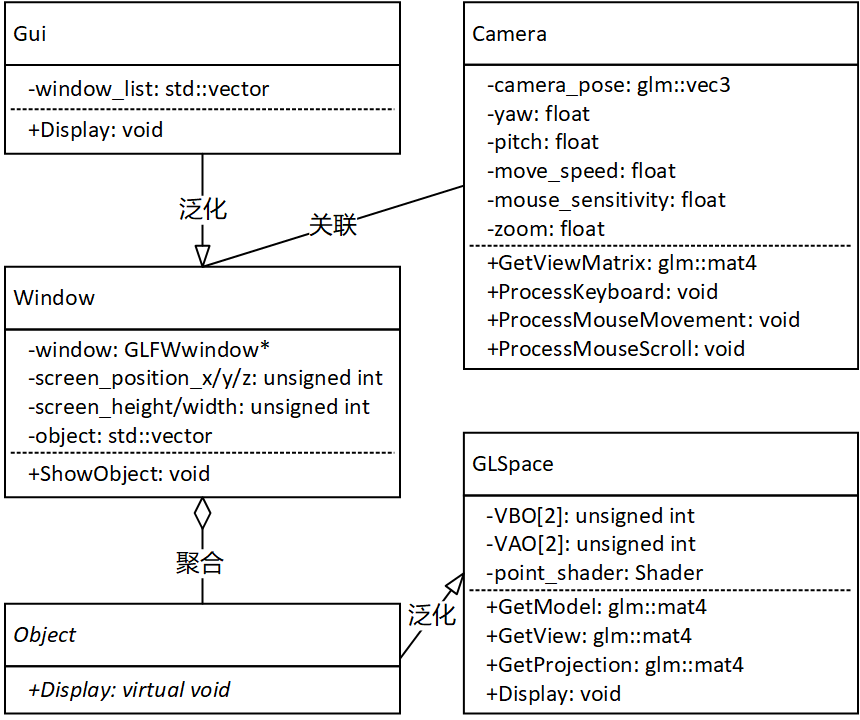
\includegraphics[width=0.7\textwidth]{figures/uml/class5.png}
	\caption{可视化模块类图}
	\label{fig:class5}
\end{figure}

\begin{table}[htbp]
	\centering
	\caption{Gui类的主要成员和方法}
	\label{table:Gui}
	\begin{tabular}{|l|m{3cm}|m{5cm}|m{4cm}|}
		\hline
		   & \multicolumn{1}{c|}{名称}                & \multicolumn{1}{c|}{类型}                                                   & \multicolumn{1}{c|}{功能}        \\
		\hline
		成员 & \centering\arraybackslash window\_list & \centering\arraybackslash vector\textless{}GLFWwindow*\textgreater{} & \centering\arraybackslash 窗口队列 \\
		\hline
		方法 & \centering\arraybackslash  Display     & \centering\arraybackslash void                                            & \centering\arraybackslash 展示窗口 \\
		\hline
	\end{tabular}
\end{table}

\begin{table}[htbp]
	\centering
	\caption{Window类的主要成员和方法}
	\label{table:Window}
	\begin{tabular}{|l|m{3cm}|m{4cm}|m{5cm}|}
		\hline
		                    & \multicolumn{1}{c|}{名称}                       & \multicolumn{1}{c|}{类型}                                               & \multicolumn{1}{c|}{功能}                           \\ \hline
		\multirow{6}{*}{成员} & \centering\arraybackslash window              & \centering\arraybackslash GLFWwindow                                  & \centering\arraybackslash 动画窗口                    \\ \cline{2-4}
		                    & \centering\arraybackslash screen\_position\_x & \centering\arraybackslash unsigned int                                & \centering\arraybackslash \multirow{2}{*}{窗口中心坐标} \\ \cline{2-3}
		                    & \centering\arraybackslash screen\_position\_y & \centering\arraybackslash unsigned int                                &                                                   \\ \cline{2-4}
		                    & \centering\arraybackslash screen\_width       & \centering\arraybackslash unsigned int                                & \centering\arraybackslash \multirow{2}{*}{窗口尺寸}   \\ \cline{2-3}
		                    & \centering\arraybackslash screen\_height      & \centering\arraybackslash unsigned int                                &                                                   \\ \cline{2-4}
		                    & \centering\arraybackslash object              & \centering\arraybackslash vector\textless{}Object*\textgreater{} & \centering\arraybackslash 需要可视化的物体                \\ \hline
		\multirow{1}{*}{方法} & \centering\arraybackslash ShowObject          & \centering\arraybackslash void                                        & \centering\arraybackslash 对物体进行可视化                \\ \hline
	\end{tabular}
\end{table}

\begin{table}[htbp]
	\centering
	\caption{GLSpace类的主要成员和方法}
	\label{table:GLSpace}
	\begin{tabular}{|l|m{3cm}|m{4cm}|m{5cm}|}
		\hline
		                    & \multicolumn{1}{c|}{名称}                 & \multicolumn{1}{c|}{类型}                & \multicolumn{1}{c|}{功能}          \\ \hline
		\multirow{3}{*}{成员} & \centering\arraybackslash VBO{[}2{]}    & \centering\arraybackslash unsigned int & \centering\arraybackslash 顶点缓冲对象 \\ \cline{2-4}
		                    & \centering\arraybackslash VAO{[}2{]}    & \centering\arraybackslash unsigned int & \centering\arraybackslash 顶点数组对象 \\ \cline{2-4}
		                    & \centering\arraybackslash point\_shader & \centering\arraybackslash Shader       & \centering\arraybackslash 着色器    \\ \hline
		\multirow{4}{*}{方法} & \centering\arraybackslash GetModel      & \centering\arraybackslash glm::mat4    & \centering\arraybackslash 计算模型矩阵 \\ \cline{2-4}
		                    & \centering\arraybackslash GetView       & \centering\arraybackslash glm::mat4    & \centering\arraybackslash 计算视图矩阵 \\ \cline{2-4}
		                    & \centering\arraybackslash GetProjection & \centering\arraybackslash glm::mat4    & \centering\arraybackslash 计算投影矩阵 \\ \cline{2-4}
		                    & \centering\arraybackslash Display       & \centering\arraybackslash void         & \centering\arraybackslash 绘制动画   \\ \hline
	\end{tabular}
\end{table}

\begin{table}[htb]
	\centering
	\caption{Camera类的主要成员和方法}
	\label{table:Camera}
	\begin{tabular}{|l|m{4cm}|m{3cm}|m{5cm}|}
		\hline
		                     & \multicolumn{1}{c|}{名称}                        & \multicolumn{1}{c|}{类型}             & \multicolumn{1}{c|}{功能}                         \\ \hline
		\multirow{10}{*}{成员} & \centering\arraybackslash position             & \centering\arraybackslash glm::vec3 & \centering\arraybackslash \multirow{5}{*}{相机位姿} \\ \cline{2-3}
		                     & \centering\arraybackslash front                & \centering\arraybackslash glm::vec3 &                                                 \\ \cline{2-3}
		                     & \centering\arraybackslash up                   & \centering\arraybackslash glm::vec3 &                                                 \\ \cline{2-3}
		                     & \centering\arraybackslash right                & \centering\arraybackslash glm::vec3 &                                                 \\ \cline{2-3}
		                     & \centering\arraybackslash world\_up            & \centering\arraybackslash glm::vec3 &                                                 \\ \cline{2-4}
		                     & \centering\arraybackslash yaw                  & \centering\arraybackslash float     & \centering\arraybackslash 偏航角                   \\ \cline{2-4}
		                     & \centering\arraybackslash pitch                & \centering\arraybackslash float     & \centering\arraybackslash 俯仰角                   \\ \cline{2-4}
		                     & \centering\arraybackslash move\_speed          & \centering\arraybackslash float     & \centering\arraybackslash 相机移动速度                \\ \cline{2-4}
		                     & \centering\arraybackslash mouse\_sensitivity   & \centering\arraybackslash float     & \centering\arraybackslash 鼠标敏感度                 \\ \cline{2-4}
		                     & \centering\arraybackslash zoom                 & \centering\arraybackslash float     & \centering\arraybackslash 缩放级别                  \\ \hline
		\multirow{4}{*}{方法}  & \centering\arraybackslash GetViewMatrix        & \centering\arraybackslash glm::mat4 & \centering\arraybackslash 获取视图矩阵                \\ \cline{2-4}
		                     & \centering\arraybackslash ProcessKeyboard      & \centering\arraybackslash void      & \centering\arraybackslash 处理键盘输入                \\ \cline{2-4}
		                     & \centering\arraybackslash ProcessMouseMovement & \centering\arraybackslash void      & \centering\arraybackslash 处理鼠标移动                \\ \cline{2-4}
		                     & \centering\arraybackslash ProcessMouseScroll   & \centering\arraybackslash void      & \centering\arraybackslash 处理鼠标滚轮                \\ \hline
	\end{tabular}
\end{table}

\par 系统的可视化模块由\texttt{Gui}类管理,\texttt{Gui}类负责管理所有的\texttt{Window}实例化对象。每个\texttt{Window}对象代表一个
独立的动画窗口,每个窗口内展示的对象都是\texttt{Object}类或其子类的实例。在这个系统中,\texttt{Window}类将
实例化两个对象,分别命名为\texttt{rgb\_win}和\texttt{semantic\_win},分别对应用于展示RGB信息和语义信息的
动画窗口。每个\texttt{Window}对象都有一个指向全局相机\texttt{Camera}的指针,这个全局相机模拟OpenGL窗口的相机,
将三维空间通过模型-视图-投影(Model-View-Projection,MVP)矩阵变换转换成二维空间,以便在屏幕上显示。
\texttt{Camera}实例化了一系列控制相机视角和位置的参数,以及一系列处理输入和移动的函数。使用统一的全局相机,可以实现RGB动画和语义动画的实时同步。

\begin{figure}[htb]
	\centering
	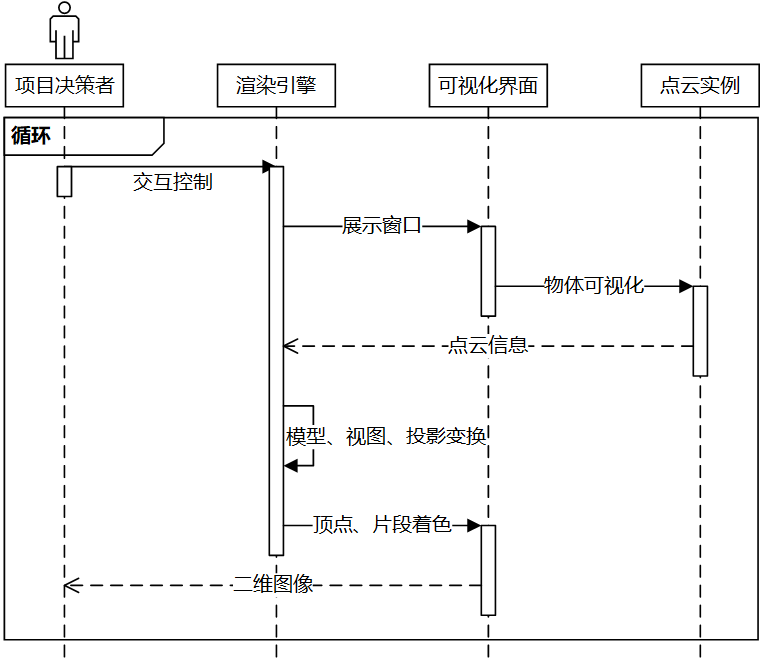
\includegraphics[width=0.7\textwidth]{figures/uml/sequence5.png}
	\caption{可视化模块时序图}
	\label{fig:sequence5}
\end{figure}

\par 为了在窗口中展示点云模型,系统实现了\texttt{GLSpace}类。这个类双继承自\texttt{Object}类和\texttt{Space}类。
\texttt{GLSpace}类实现了\texttt{Display}函数,用于绘制动画,包括点云模型和相机位姿,伪代码算法\ref{algo:Display}所示。同时,它还实现了一系列
计算矩阵的函数,这些函数负责计算模型、视图和投影矩阵。\texttt{GLSpace}类只实例化一个对象,负责在窗口中展示\texttt{Space}对象的点云模型。

\begin{algorithm}[htbp]
	\SetAlgoLined
	\KwData{动画窗口 window}
	\KwResult{点云动画}
	$\textit{点云着色器 point\_shader} \gets \text{顶点着色器 vertex\_shader,片元着色器 fragment\_shader}$\;
	$\text{初始化VBO, VAO}$\;
	$\text{初始化 current\_point\_num 为 0}$\;
	$\text{绑定VAO和VBO}$\;
	\tcp{设置点云的坐标}
	$\text{glVertexAttribPointer}(0, 3, GL\_FLOAT, 0, 6 * \text{sizeof(float)}, (void *)0)$\;
	\tcp{设置点云的颜色}
	$\text{glVertexAttribPointer}(1, 3, GL\_FLOAT, 0, 6 * \text{sizeof(float)}, (void *)(3 * sizeof(float)))$\;
	\While{\text{not} glfwWindowShouldClose(window)}{
		\If{当前窗口 == rgb\_win}{
			$\text{根据两帧间的时间差获取当前帧}$\;
			$\text{计算deltaTime并更新lastFrame}$\;
		}
		$\text{处理窗口的键盘输入}$\;
		$\text{清除颜色和深度缓冲}$\;
		$\text{设置点大小并绘制点}$\;
		\tcp{更新摄像机位置,实质上为每个点计算MVP矩阵}
		$\text{计算MVP矩阵}$\;
		$\text{在 point\_shader 中设置MVP矩阵}$\;
		$\text{设置点大小并绘制点}$\;
		\If{gl\_data\_mtx 未上锁}{
			\If{轮到当前窗口从点云数组中读取数据}{
				$\text{更新 current\_point\_num}$\;
				$\text{为当前窗口加载数据到缓冲对象中}$\;
			}
			$\text{解锁 gl\_data\_mtx}$\;
		}
		$\text{交换前后缓冲}$\;
		$\text{获取并处理事件}$\;
	}
	$\text{删除VAO和VBO}$\;
	\caption{Display}
	\label{algo:Display}
\end{algorithm}

\par 在可视化模块开始运行时,\texttt{Gui}类首先会初始化一个\texttt{Window}对象列表,这个列表存储了所有需要
展示的窗口。接着,通过\texttt{Display}逐个调用列表中每个\texttt{Window}对象的\texttt{ShowObject}函数,展示每个窗
口中的\texttt{Object}对象。这里的\texttt{Object}包括\texttt{GLSpace}类的实例,以及展示相机朝向的向量。

\par \texttt{GLSpace}类同样包含\texttt{Display},负责在\texttt{OpenGL}窗口中绘制出实例化对象。\texttt{Display}首先使用\texttt{VBO}和
\texttt{VAO}在GPU中创建缓冲区,然后使用\texttt{Shader}类加载顶点着色器和片段着色器,最后通过\texttt{GetProjection}、
\texttt{GetView}和\texttt{GetModel}函数计算出MVP矩阵,将三维空间的点云模型投影到二维屏幕上。

\par 为了保证渲染的实时性,数据传输模块会使用双缓冲技术,将点云生成与语义融合模块生成的新
数据传输到OpenGL的缓冲区中,同时,已经在屏幕上显示的旧数据会被保留在另一个缓冲区中,这样可
以防止新旧数据之间的冲突,同时提高渲染的效率。

\par 为了实现交互控制,用户可以通过键盘和鼠标输入,调整相机的位置和视角。\texttt{Camera}的
\texttt{ProcessKeyboard}、\texttt{ProcessMouseMovement}和\texttt{ProcessMouseScroll}函数会根据用户输入的方向、
位移和滚动量,动态调整相机的参数,从而改变相机的位姿和视角。

\par 为了提高可视化的性能,系统可以采用多线程技术并行处理数据,创建两个子线程分别展示RGB动画窗口和语义动画窗口。后续还可以使用GPU加速渲染,通过使用NVIDIA官方提供的\href{https://docs.nvidia.com/cuda/cuda-runtime-api/group__CUDART__OPENGL.html#group__CUDART__OPENGL}{OpenGL Interoperability 系列 API},可以提高系统的渲染效率,提升用户体验。
\subsection{点云后处理模块}
\par 该模块对输入的点云数据,包含每个点的全局三维坐标、RGB值和类别标签进行处理,组件图如图\ref{fig:component6}所示,时序图如图\ref{fig:sequence7}所示。

\begin{figure}[htb]
	\centering
	\begin{minipage}[t]{0.42\textwidth}
		\centering
		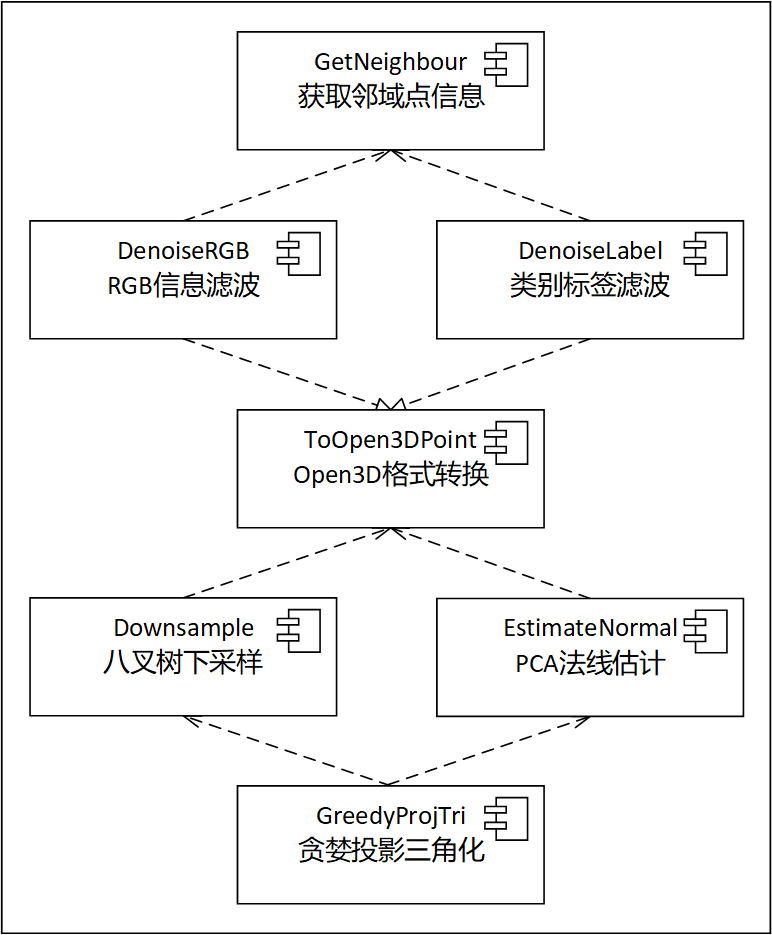
\includegraphics[height=7.5cm,keepaspectratio]{figures/uml/component6.png}
		\caption{点云后处理模块组件图}
		\label{fig:component6}
	\end{minipage}
	\begin{minipage}[t]{0.53\textwidth}
		\centering
		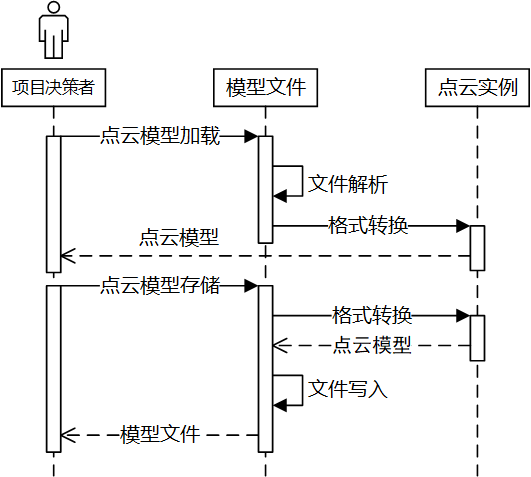
\includegraphics[height=7.5cm,keepaspectratio]{figures/uml/sequence7.png}
		\caption{模型导入导出模块时序图}
		\label{fig:sequence7}
	\end{minipage}
\end{figure}

\par 点云模型重建完成后,首先进行点云的降噪操作。在室内重建中,由于噪声点和离群点的存在,
会对模型质量产生影响。因此,使用基于局部密度的滤波方法进行降噪可以在去除噪声的同时保留边缘
信息。\texttt{Space}类定义了函数\texttt{GetNeighbour}、\texttt{DenoiseRGB}和\texttt{DenoiseLabel},用于获取点的邻域信息并且
对点的RGB值和类别标签进行滤波处理,邻域点集类别标签的多数可以由算法\ref{algo:GetMajorityLabel}得到,每个点的序号可以由公式\ref{get_neighbour}计算出:
\begin{equation}
	\begin{aligned}
		& \texttt{Left}   &  & = (\texttt{blockIdx} \times \texttt{blockDim} + \texttt{threadIdx}) \times \texttt{n} + \texttt{i} - 1       \\
		& \texttt{Right}  &  & = (\texttt{blockIdx} \times \texttt{blockDim} + \texttt{threadIdx}) \times \texttt{n} + \texttt{i} + 1       \\
		& \texttt{Up}     &  & = (\texttt{blockIdx} \times \texttt{blockDim} + \texttt{threadIdx} + 1) \times \texttt{n} + \texttt{i}       \\
		& \texttt{Down}   &  & = (\texttt{blockIdx} \times \texttt{blockDim} + \texttt{threadIdx} - 1) \times \texttt{n} + \texttt{i}       \\
		& \texttt{Front}  &  & = ((\texttt{blockIdx} + 1) \times \texttt{blockDim} + \texttt{threadIdx}) \times \texttt{n} + \texttt{i} - 1 \\
		& \texttt{Behind} &  & = ((\texttt{blockIdx} - 1) \times \texttt{blockDim} + \texttt{threadIdx}) \times \texttt{n} + \texttt{i} - 1 \\
	\end{aligned}
	\label{get_neighbour}
\end{equation}
其中,$\texttt{n}$ 为点云数组 $\texttt{point\_list}$ 的长度,$\texttt{i}$ 为当前点在点云数组中的序号。

\begin{algorithm}[htb]
	\SetAlgoLined
	\KwData{领域点集 neighbor\_point[], 类别标签集合 list[]}
	\KwResult{多数标签 majority\_label}
	初始化整数数组 $count[27]$ 用于计算领域点集标签的数量\;
	初始化 $num = 0$\;
	\For{$i$ in 领域点集中所有的点}{
		\If{not $neighbor\_point[i]$}{
			继续下一次循环\;
		}
		$count[int(list[i])]++$\;
		\If{$count[int(list[i])] > num$}{
			$num = count[int(list[i])]$\;
			$majority\_label = list[i]$\;
		}
	}
	\caption{GetMajorityLabel}
	\label{algo:GetMajorityLabel}
\end{algorithm}

\par 降噪完成后,可选择进行点云的下采样、法线估计和曲面重建操作。为了更好地实现这些功能,
系统通过\texttt{ToOpen3DPointCloud}把点云数据转换成Open3D库可以处理的格式。函数遍历\texttt{point\_list}数组中所
有的点。对于每个点,它将点的世界坐标 $P_w$ 添加到\texttt{points}数组,将点的RGB值添加到\texttt{colors}数组。

\par \texttt{Downsample}实现了基于八叉树的下采样方法。首先,使用Open3D的\texttt{VoxelDownSample}
方法对点云进行下采样,得到\texttt{voxel\_down\_pcd}点云。接着,清空原始点云\texttt{pcd}的\texttt{points}和\texttt{colors}
数组。然后,遍历下采样后的点云,将每个点的坐标和颜色添加到原始点云\texttt{pcd}中。这一步骤可以
有效地降低点云数据的规模,减少存储和计算成本,同时保留了点云的主要结构信息。

% \begin{figure}[htb]
% 	\centering
% 	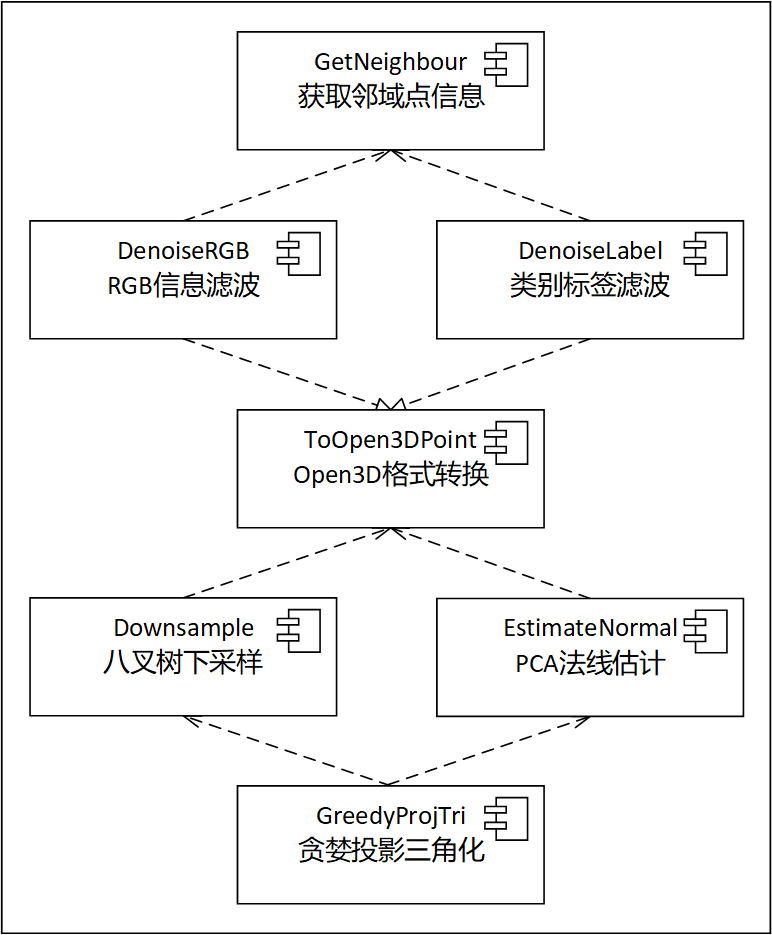
\includegraphics[width=0.7\textwidth]{figures/uml/component6.png}
% 	\caption{点云后处理模块组件图}
% 	\label{fig:component6}
% \end{figure}

% \begin{figure}[htbp]
% 	\centering
% 	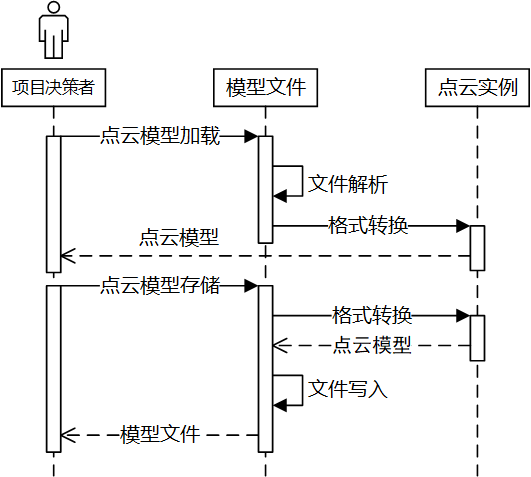
\includegraphics[width=0.618\textwidth]{figures/uml/sequence7.png}
% 	\caption{模型导入导出模块时序图}
% 	\label{fig:sequence7}
% \end{figure}



\par 下采样操作完成后,可以根据需要选择进行表面法线的估计。\texttt{EstimateNormal}实现了基于主成分
分析的法线估计方法。首先,初始化一个协方差矩阵和质心向量。然后,对邻居点进行遍历,
累加每个点的坐标,得到总坐标值后计算平均坐标,也就是质心。接着,再次遍历邻居点,计算每个点
的坐标减去质心的差,然后将其外积添加到协方差矩阵。最后,使用主成分分析算法求解协方差矩阵的特征向
量和特征值,返回特征值最小对应的特征向量,即为点云的法线。

\par 最后,可以选择进行曲面的重建操作。\texttt{GreedyProjTri}调用Open3D库的
\texttt{create\_from\_point\_cloud\_poisson}方法,通过贪婪投影三角化的算法,在给定的半径和最大最近邻距离参数下,对点云进行
三角化处理,生成并返回一个三角形网格。

\subsection{模型导入导出模块}

\par 每当需要加载一个新的模型时,首先调用\texttt{Space}类的\texttt{LoadCloud}函数,将通过文件读取接口打开
指定的点云模型文件,然后解析PLY文件头部,获取其中的关键信息,如格式、元素类型、属性等。接
下来,文件读取接口会解析文件的数据部分,提取每个顶点的坐标、RGB值以及类别标签,存入
\texttt{point\_list}数组中。最后,关闭文件,完成模型的导入。

\par 以上步骤完成后,系统便完成了模型的导入过程,可以使用导入的模型进行后续的三维重建和语
义分割工作。

\begin{algorithm}[htbp]
    \SetAlgoLined
    \KwData{场景序号 scene\_id, 点云结构体数组 point\_list}
	\KwResult{模型文件 file}
    $\textit{file\_name} \gets \text{'../pred/'} + \textit{scene\_id} + \text{'.ply'}$\;
    $\textit{file} \gets \text{open}(\textit{file\_name}, \text{'w'})$\;

    $\textit{header} \gets \text{'ply'}$\;
    $\textit{header} \gets \text{'format binary\_little\_endian 1.0'}$\;
    $\textit{header} \gets \text{'element vertex'} + \textit{gl\_point\_num}$\;
    $\textit{header} \gets \text{'property float x'} + \text{'property float y'} + \text{'property float z'}$\;
    $\textit{header} \gets \text{'property uchar color\_r'} + \text{'property uchar color\_g'} + \text{'property uchar color\_b'}$\;
    $\textit{header} \gets \text{'property uchar label\_r'} + \text{'property uchar label\_g'} + \text{'property uchar label\_b'}$\;
    $\textit{header} \gets \text{'property int label'}$\;
    $\textit{header} \gets \text{'element face 7'}$\;
    $\textit{header} \gets \text{'end\_header'}$\;
    $\text{write\_to\_file}(\textit{file}, \textit{header})$\;

    \For{$point\_list$ 中的每个点 $\textit{p}$}{
        使用 $\textit{pose}$ 计算变换后的坐标 $\textit{x, y, z}$\;
        $\text{write\_to\_file}(\textit{file}, \textit{x, y, z})$\;
        从 $\textit{p}$ 中获取并缩放RGB值 $\textit{color\_r, color\_g, color\_b}$\;
        $\text{write\_to\_file}(\textit{file}, \textit{color\_r, color\_g, color\_b})$\;
        $\textit{label} \gets \textit{p}$ 的标签\;
        $\text{write\_to\_file}(\textit{file}, \textit{label})$\;
        根据 $\textit{label}$ 检索标签对应的 RGB 值 $\textit{label\_r, label\_g, label\_b}$\;
        $\text{write\_to\_file}(\textit{file}, \textit{label\_r, label\_g, label\_b})$\;
    }
    \caption{SaveCloud}
    \label{algo:SaveCloud}
\end{algorithm}

\par 在系统运行过程中,可能需要将处理后的模型导出到文件,以便于保存结果或用于其他应用。
此时,可以调用\texttt{Space}类的\texttt{SaveCloud}函数,伪代码如算法\ref{algo:SaveCloud}所示。它主要负责将点云数据存储到一个PLY文件中。首先,
通过拼接路径和场景序号来定义文件名。然后,打开这个文件进行写操作。先写入PLY文件的头部信息,
接着,函数通过遍历点云数组\texttt{point\_list}来写入每一个点的信息。每个点的信息包括全局坐标(通过
系统坐标和位姿矩阵运算得到)、RGB值以及类别标签。在写入语义信息的同时,根据标签值,
函数会将对应的颜色编码写入文件,这个编码由ScanNet定义。最后,关闭文件,完成模型的导出。导入导出的时序图如图\ref{fig:sequence7}所示。

\par 该模块通过灵活的接口,有效地支持了系统的运行。通过这个模块,系统可以方便地
处理各种点云格式的输入输出,同时保证了几何信息和语义信息的一致性和完整性,提高了系统
的灵活性和实用性。
\subsection{用户管理模块}

\par 该模块使用\texttt{User}类(见表\ref{table:User})对所有用户进行统一的管理。系统开始运行时,首先调用\texttt{ReadCSV}函数读取指定路径的用户数据文件,将用户数据写入用户列表\texttt{user\_table}中。

\begin{table}[htb]
    \centering
    \caption{User类的主要成员和方法}
    \label{table:User}
    \begin{tabular}{|l|m{3cm}|m{4cm}|m{5cm}|}
        \hline
                            & \multicolumn{1}{c|}{名称}                & \multicolumn{1}{c|}{类型}                                        & \multicolumn{1}{c|}{功能}            \\
        \hline
        成员                  & \centering\arraybackslash user\_table  & \centering\arraybackslash map<username, tuple<password, role>> & \centering\arraybackslash 用户列表     \\ \hline
        \multirow{7}{*}{方法} & \centering\arraybackslash GetUsername  & \centering\arraybackslash string                               & \centering\arraybackslash 获取用户名    \\ \cline{2-4}
                            & \centering\arraybackslash GetRole      & \centering\arraybackslash int                                  & \centering\arraybackslash  获取用户角色  \\ \cline{2-4}
                            & \centering\arraybackslash Authenticate & \centering\arraybackslash bool                                 & \centering\arraybackslash 验证用户登录凭证 \\ \cline{2-4}
                            & \centering\arraybackslash DeleteUser   & \centering\arraybackslash void                                 & \centering\arraybackslash 删除用户     \\ \cline{2-4}
                            & \centering\arraybackslash ChangeRole   & \centering\arraybackslash void                                 & \centering\arraybackslash 修改用户角色   \\ \cline{2-4}
                            & \centering\arraybackslash ReadCSV      & \centering\arraybackslash map                                  & \centering\arraybackslash 读取用户数据文件 \\ \cline{2-4}
                            & \centering\arraybackslash WriteCSV     & \centering\arraybackslash void                                 & \centering\arraybackslash 写入用户数据文件 \\ \hline
    \end{tabular}
\end{table}

\par 用户注册功能允许新用户创建系统账户。在注册时,用户需要提供一个安全的登录凭证,包括用户名和密码。注册信息将被传送到系统,调用\texttt{Authenticate}函数进行验证,包括检查用户名是否唯一、密码是否符合安全标准。
如果符合标准,则通过\texttt{GetUsername}函数检查用户名是否已经存在于用户列表中,若不存在则写入。一旦注册成功,用户将获得系统的访问权限。
已注册的用户可以通过用户名和密码登录系统。登录成功后,用户将能够访问系统的各项功能和数据。

\par 管理员登录后,可以对任意用户账户进行删除和角色管理操作。用户角色仅限于系统操作员、数据工程师、算法研究员和项目决策者,通过\texttt{ChangeRole}修改用户列表中每个用户名对应的\texttt{role}字段可以实现角色的修改。
通过\texttt{DeleteUser}函数可以将待删除的账户移出用户列表。一旦账户被删除,用户将失去对系统的访问权限,可以确保用户数据的隐私和安全性。

\par 通过明确的用户身份验证和角色管理,系统可以有效地防止未经授权的访问和操作,从而维护数据的完整性和保密性。

\section{系统实现}
% !TeX root = ../main.tex

\subsection{开发方法}

\begin{enumerate}
	\item{面向对象开发}
	\par 采用面向对象的开发方法,自底向上的归纳,将系统的各个部分抽象为不同的类。通过定义清晰的接口和实现详细的封装,
	降低模块之间的耦合度,提高系统的可扩展性和可维护性。

	\item{可视化开发}
	\par 采用可视化开发方法。由于三维重建和语义融合产生的模型数据抽象且数据量庞大,因此在开发过程中难以直接判断系统运行的正确性。
	因此,需要首先编写出可视化模块,以实时展示和检查点云生成及语义融合更新的过程。这不仅方便开发过程中识别和修复错误,还能直观地展示开发成果。

	\item{增量开发}
	\par 由于课题组对此系统的急切需求,因此采用增量开发的方法。首先依次实现室内重建、可视化、点云生成及语义融合更新等系统的核心功能。
	在核心功能稳定运行后,再逐步添加增量式重建、曲面重建和实例融合更新等额外功能。

	\item{编码规范}
	\par 遵循 \href{https://google.github.io/styleguide/cppguide.html}{Google C++ Style Guide} 编码规范以确保编写的代码能达到预期的功能并具有高可读性。
	每个头文件都需要使用宏定义来防止被多次包含,如 Matrix.h 需要声明为 MATRIX\_H\_,且每个头文件都是自足的,不依赖于其他头文件的包含顺序。
	命名规则方面,类名采用驼峰命名法,变量和函数名使用小写字母和下划线。
	初始化方面,应遵循RAII(Resource Acquisition Is Initialization)原则,尽量使用C++的标准类型。特别是对于如Space、Frame等负责管理资源的类,需要自定义构造函数和析构函数,同时禁用拷贝函数。
	为了线程安全,存在多线程竞争的地方,例如动画窗口、数据交换等,需要使用std::mutex进行同步。
\end{enumerate}

\subsection{实现效果}

\begin{figure}[htbp]
	\centering
	\subfigure[RGB图像]{
		\begin{minipage}[t]{0.48\linewidth}
			\centering
			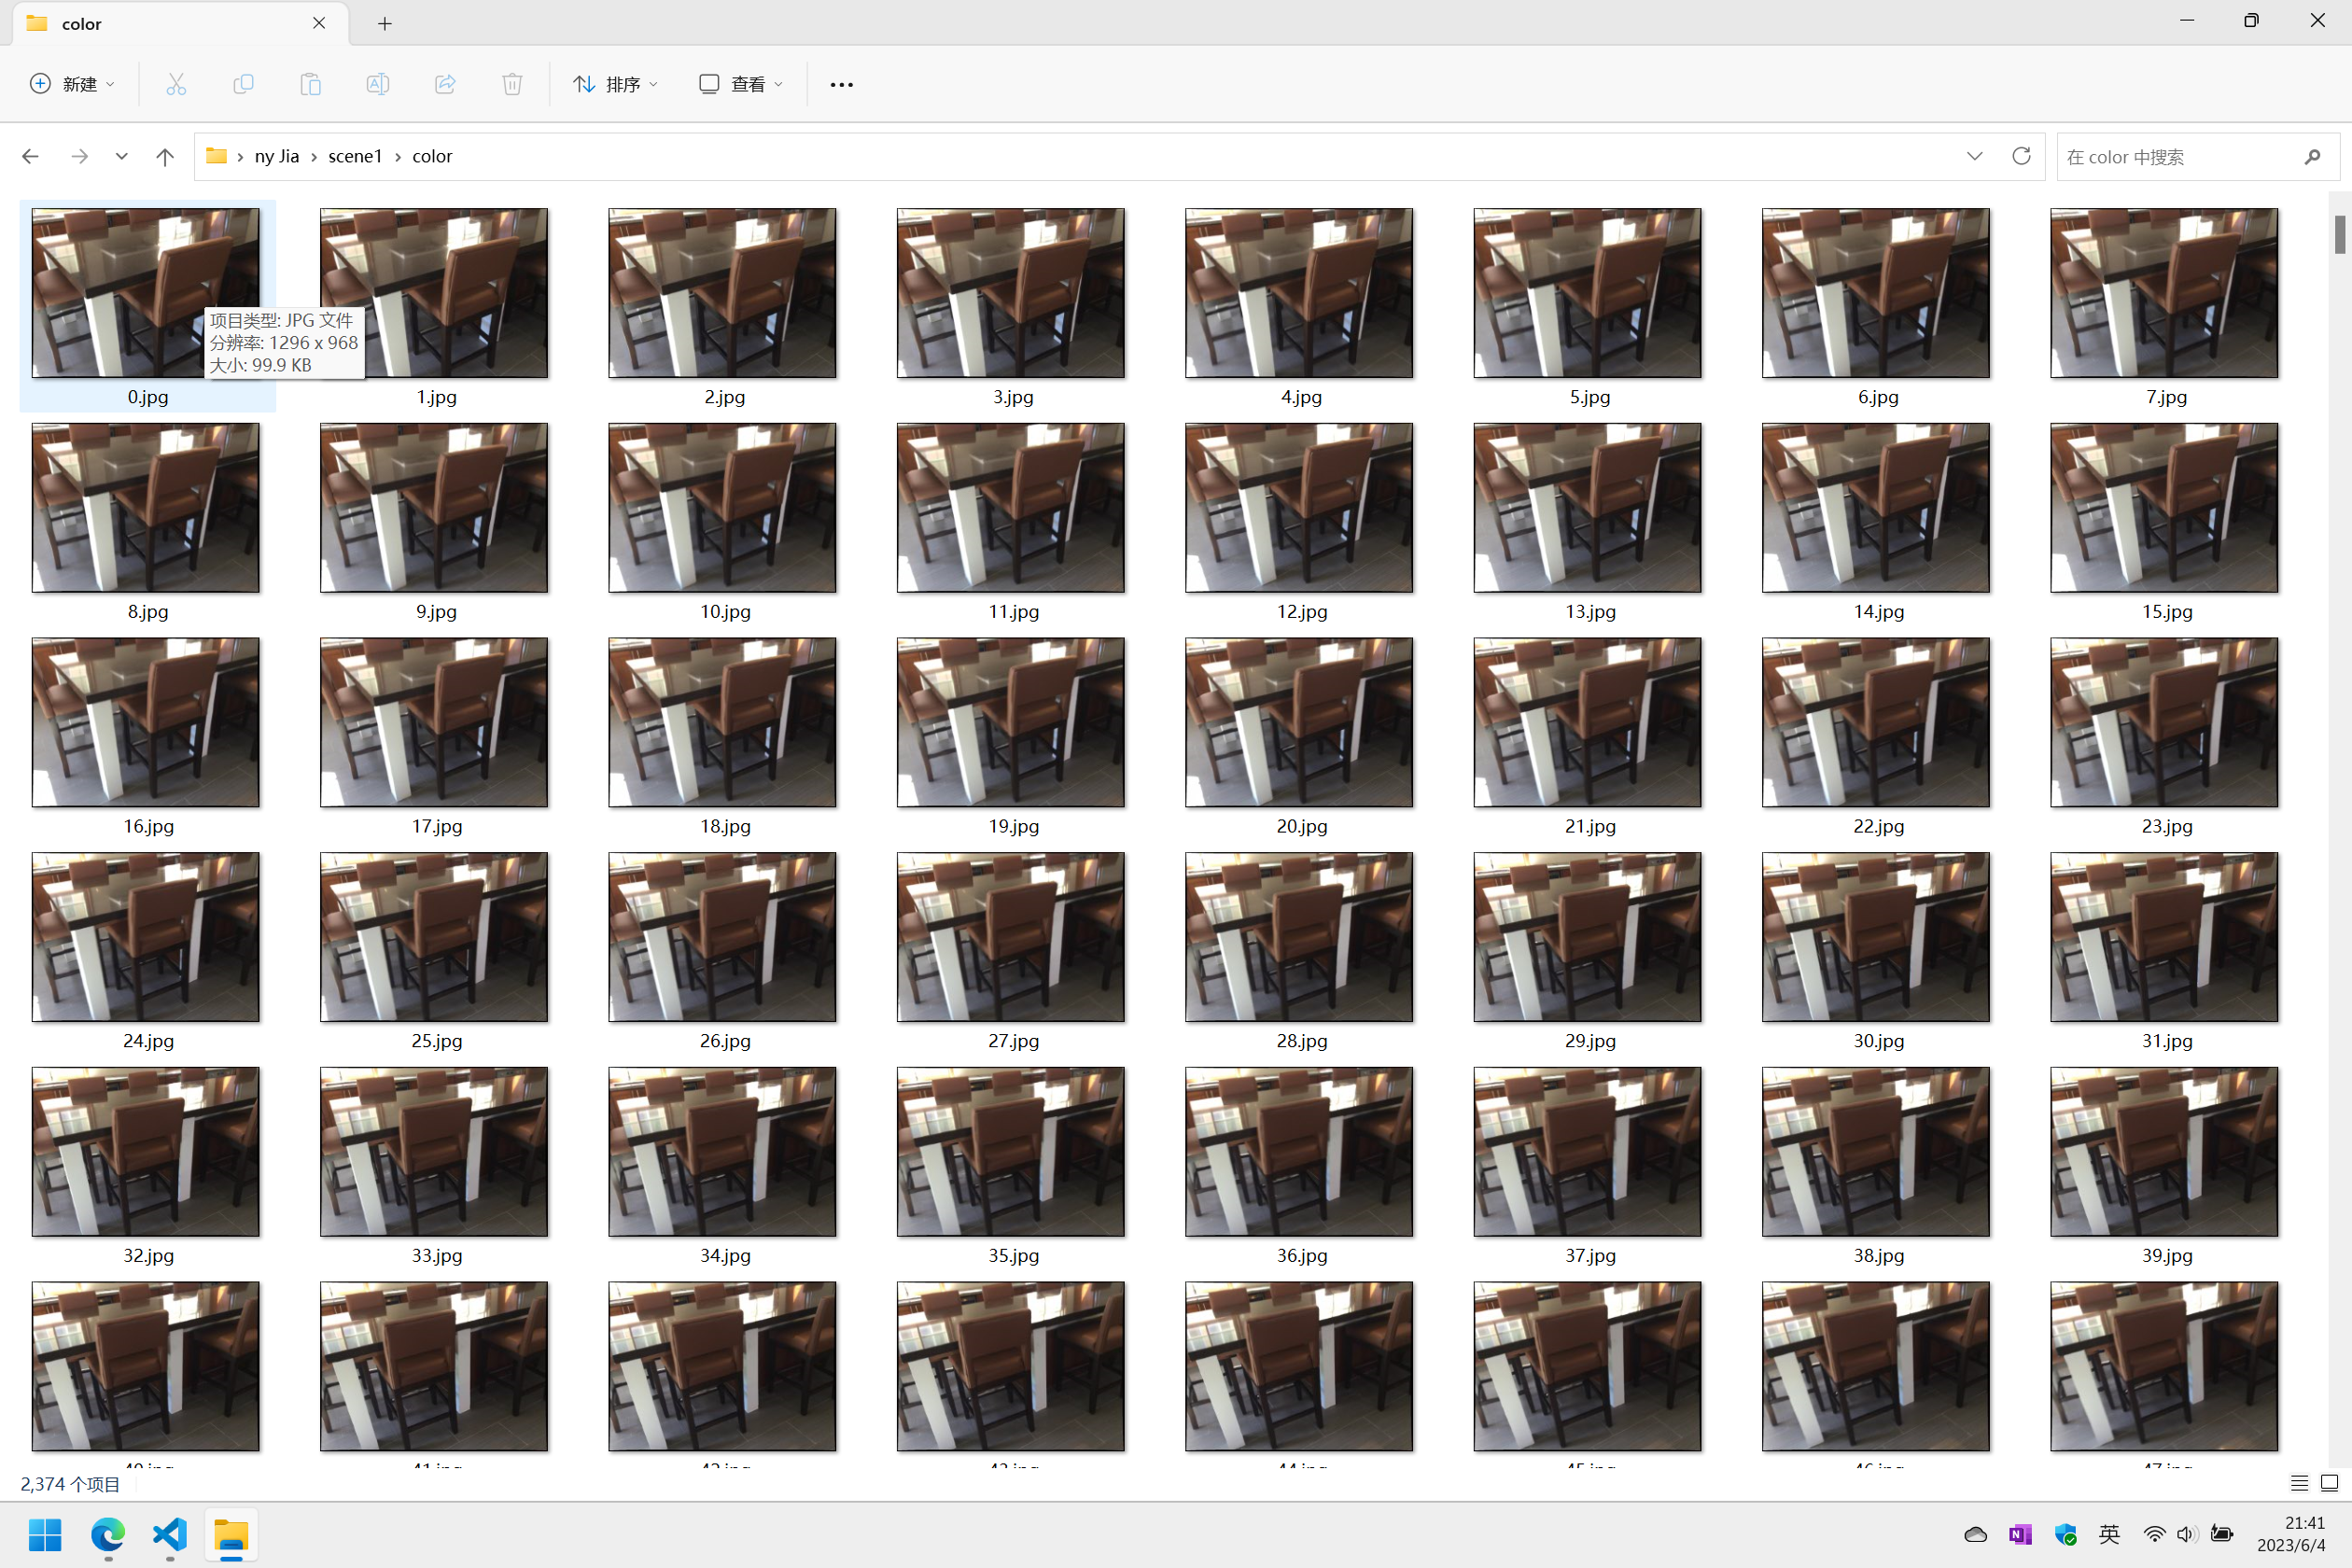
\includegraphics[width=1\textwidth]{figures/scene1_color.png}
		\end{minipage}
	}
	\subfigure[深度图像]{
		\begin{minipage}[t]{0.48\linewidth}
			\centering
			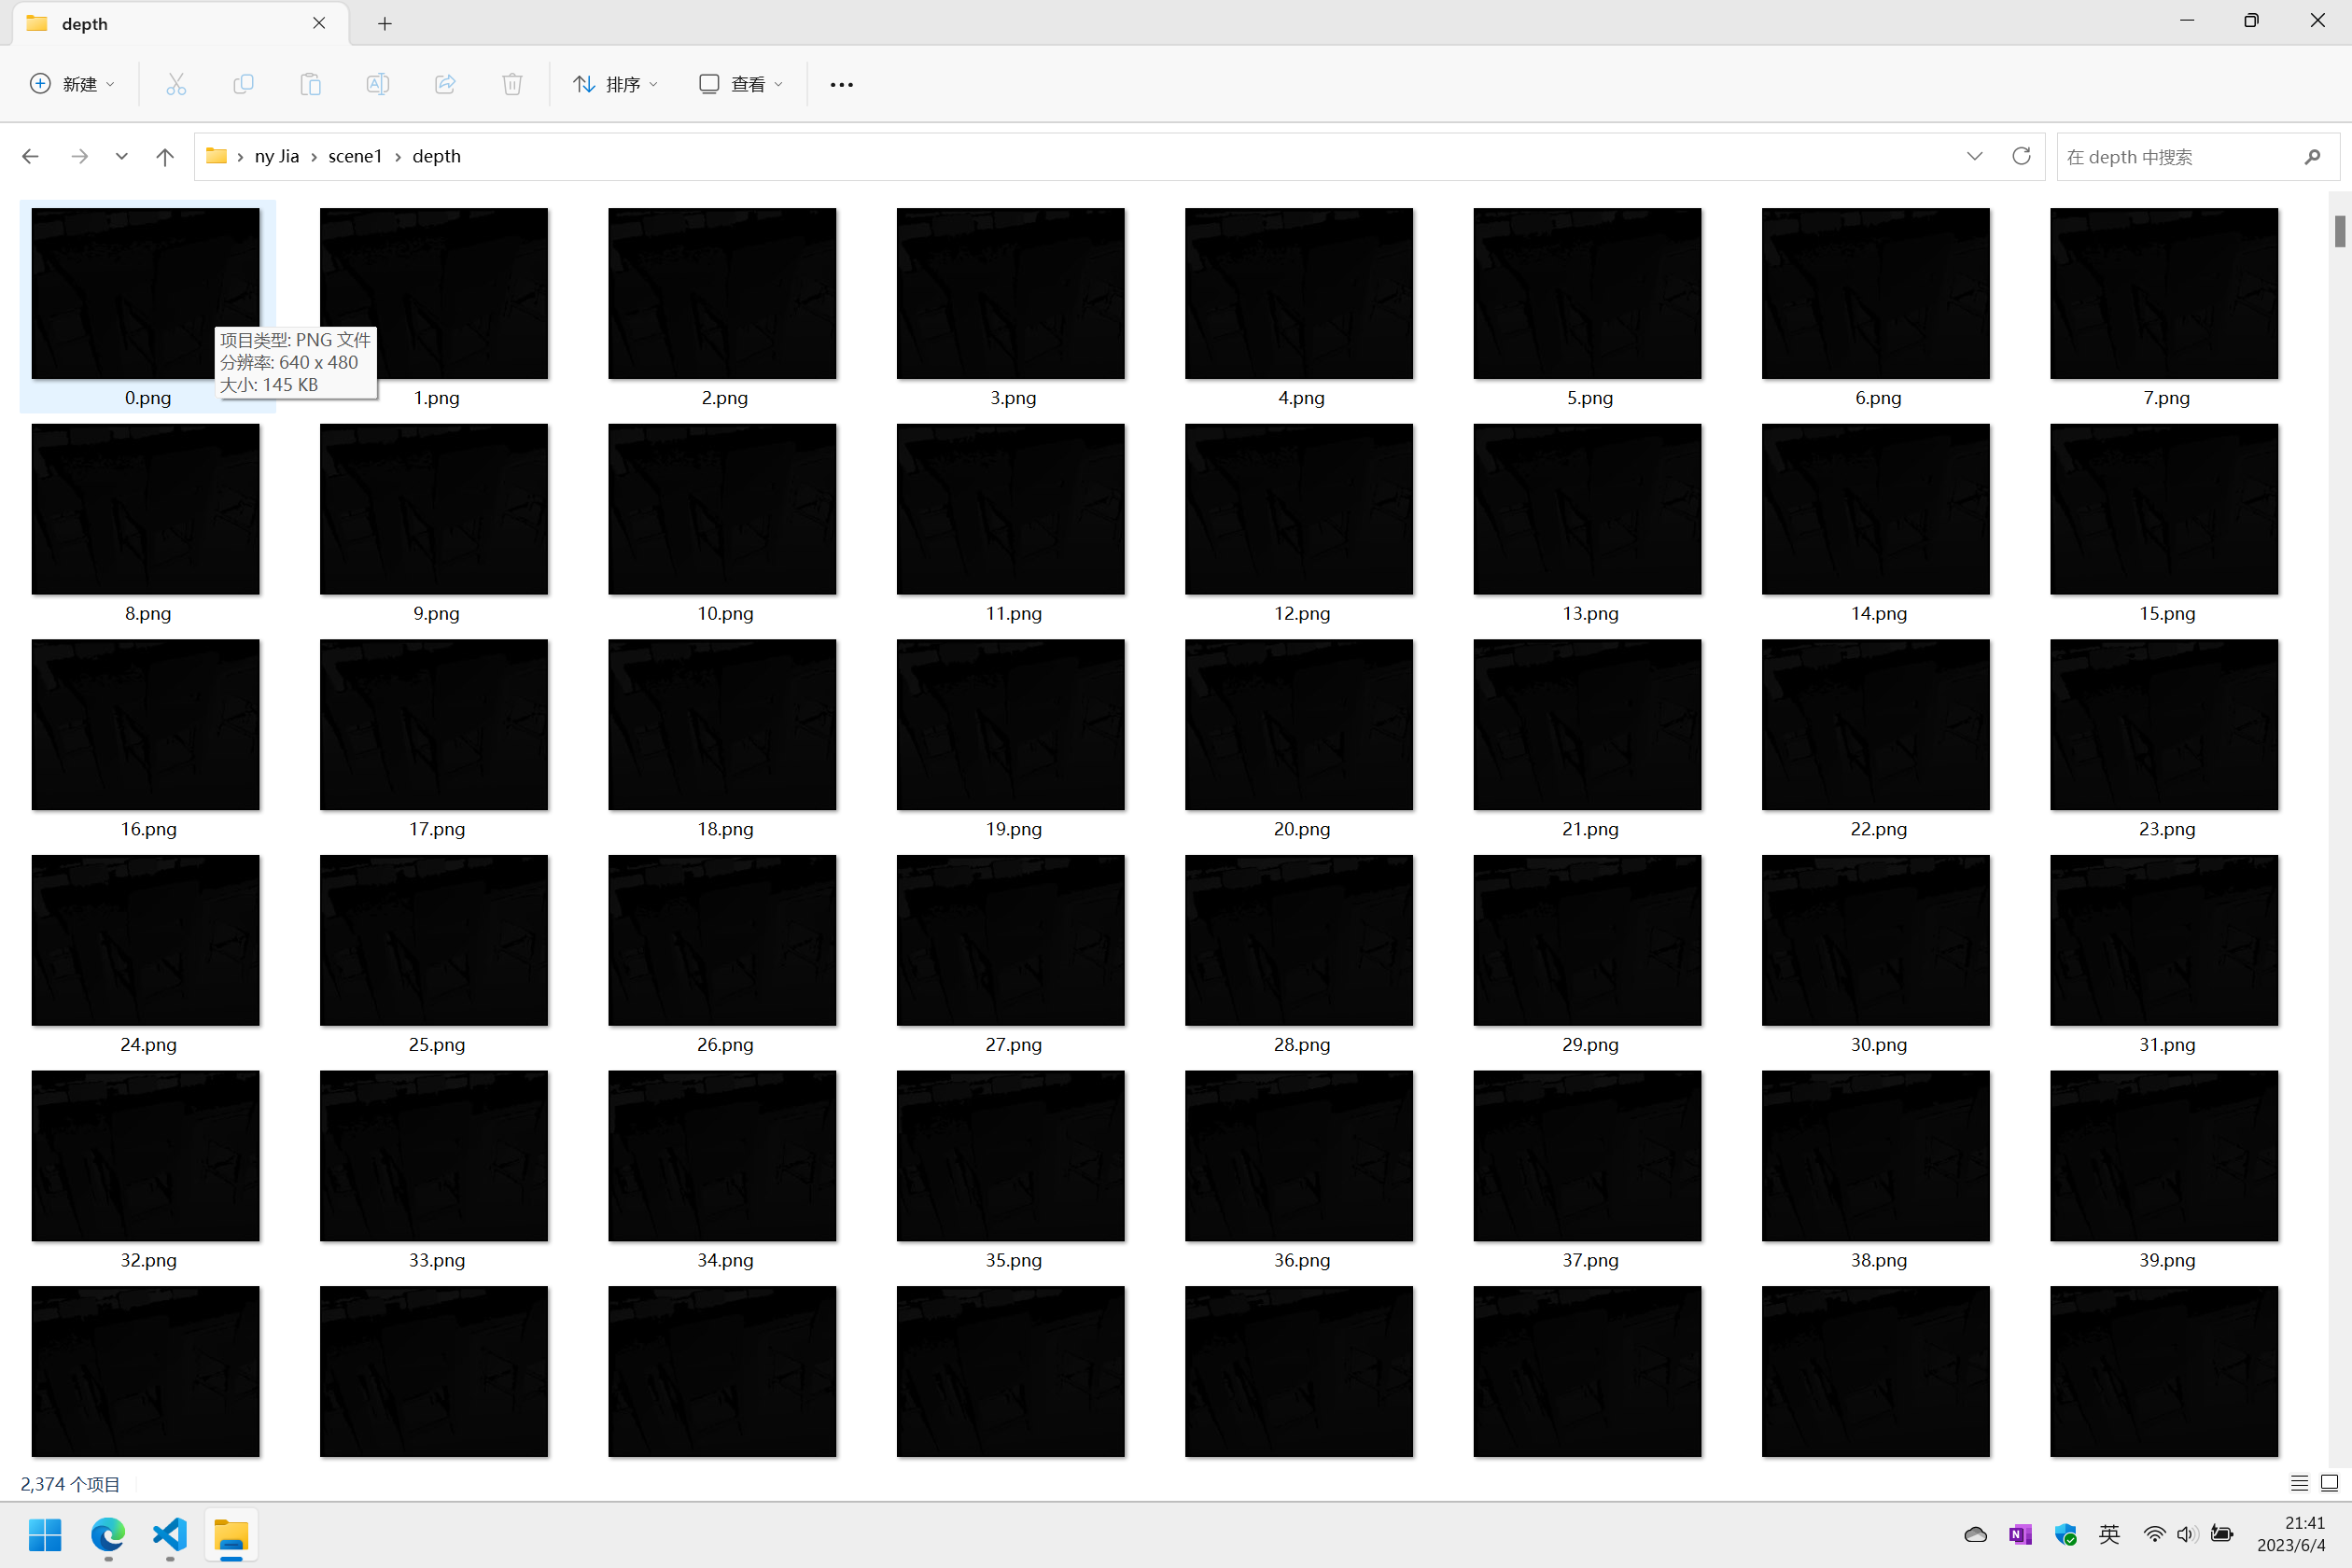
\includegraphics[width=1\textwidth]{figures/scene1_depth.png}
		\end{minipage}
	}
	\caption{数据采集结果}
	\label{fig:origin_img}
\end{figure}
\begin{figure}[htbp]
	\centering
	\begin{minipage}[t]{0.48\textwidth}
		\centering
		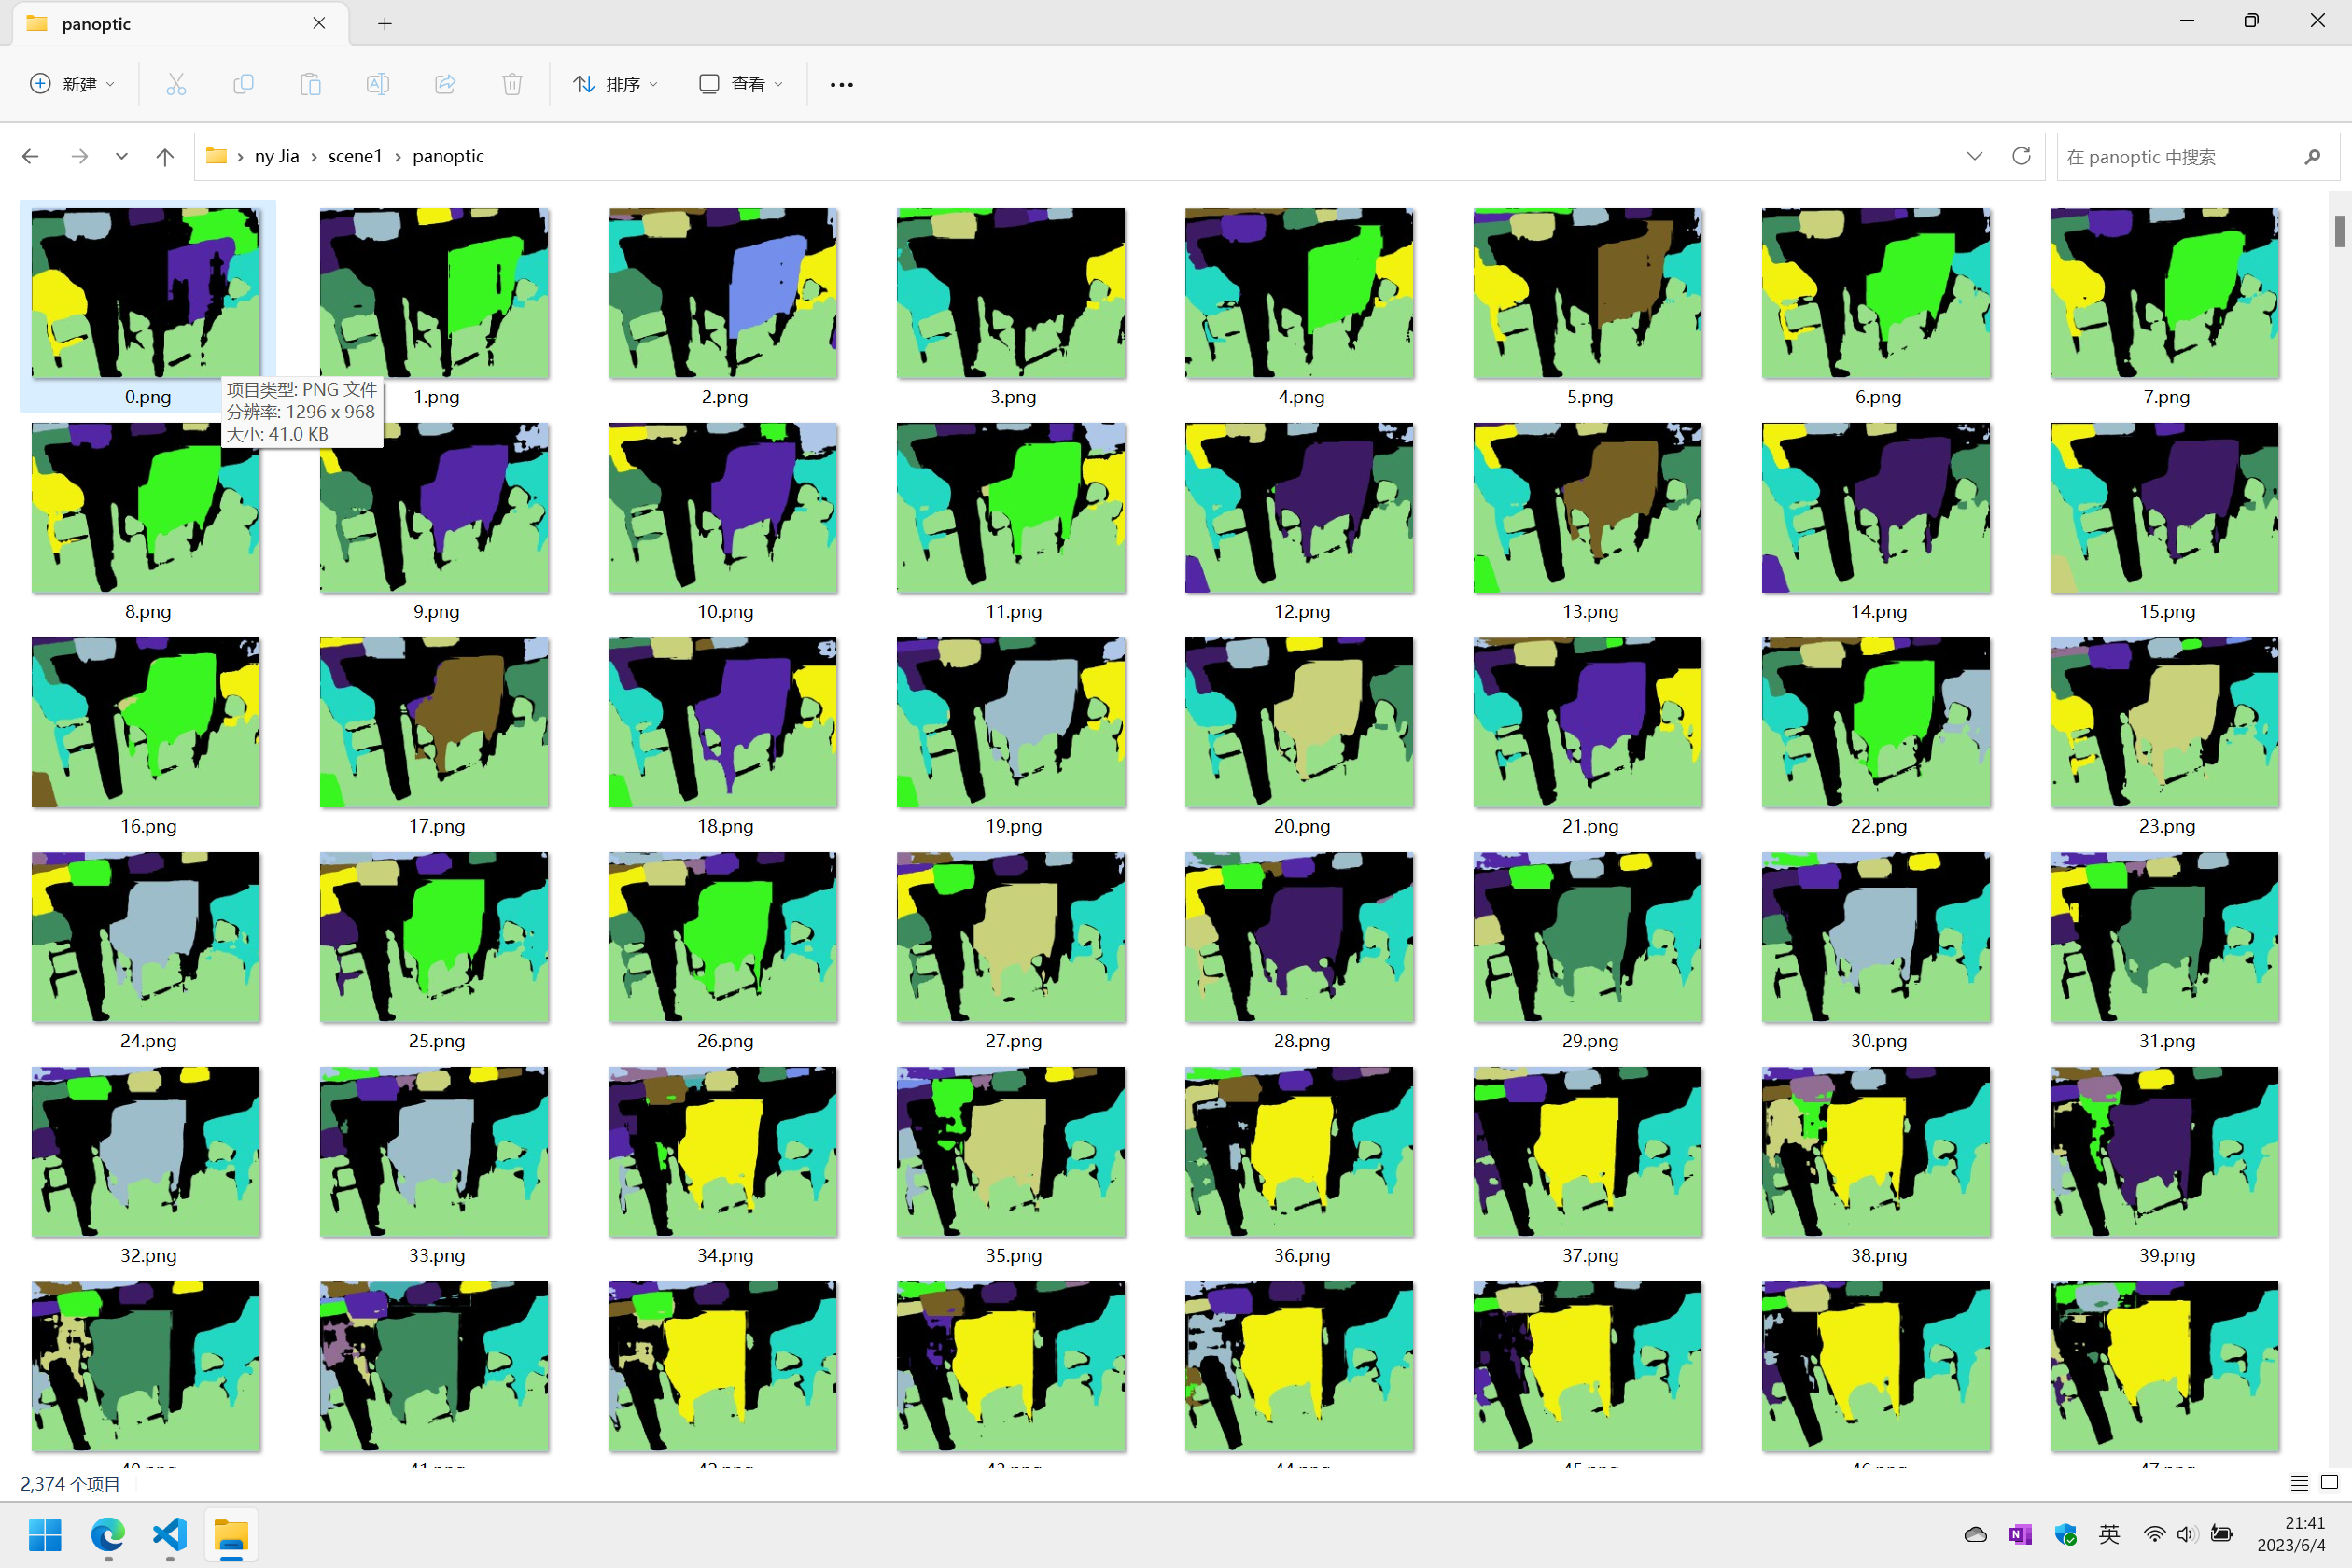
\includegraphics[width=1\textwidth]{figures/scene1_semantic.png}
		\caption{语义分割图像}
		\label{fig:seg_image}
	\end{minipage}
	\begin{minipage}[t]{0.48\textwidth}
		\centering
		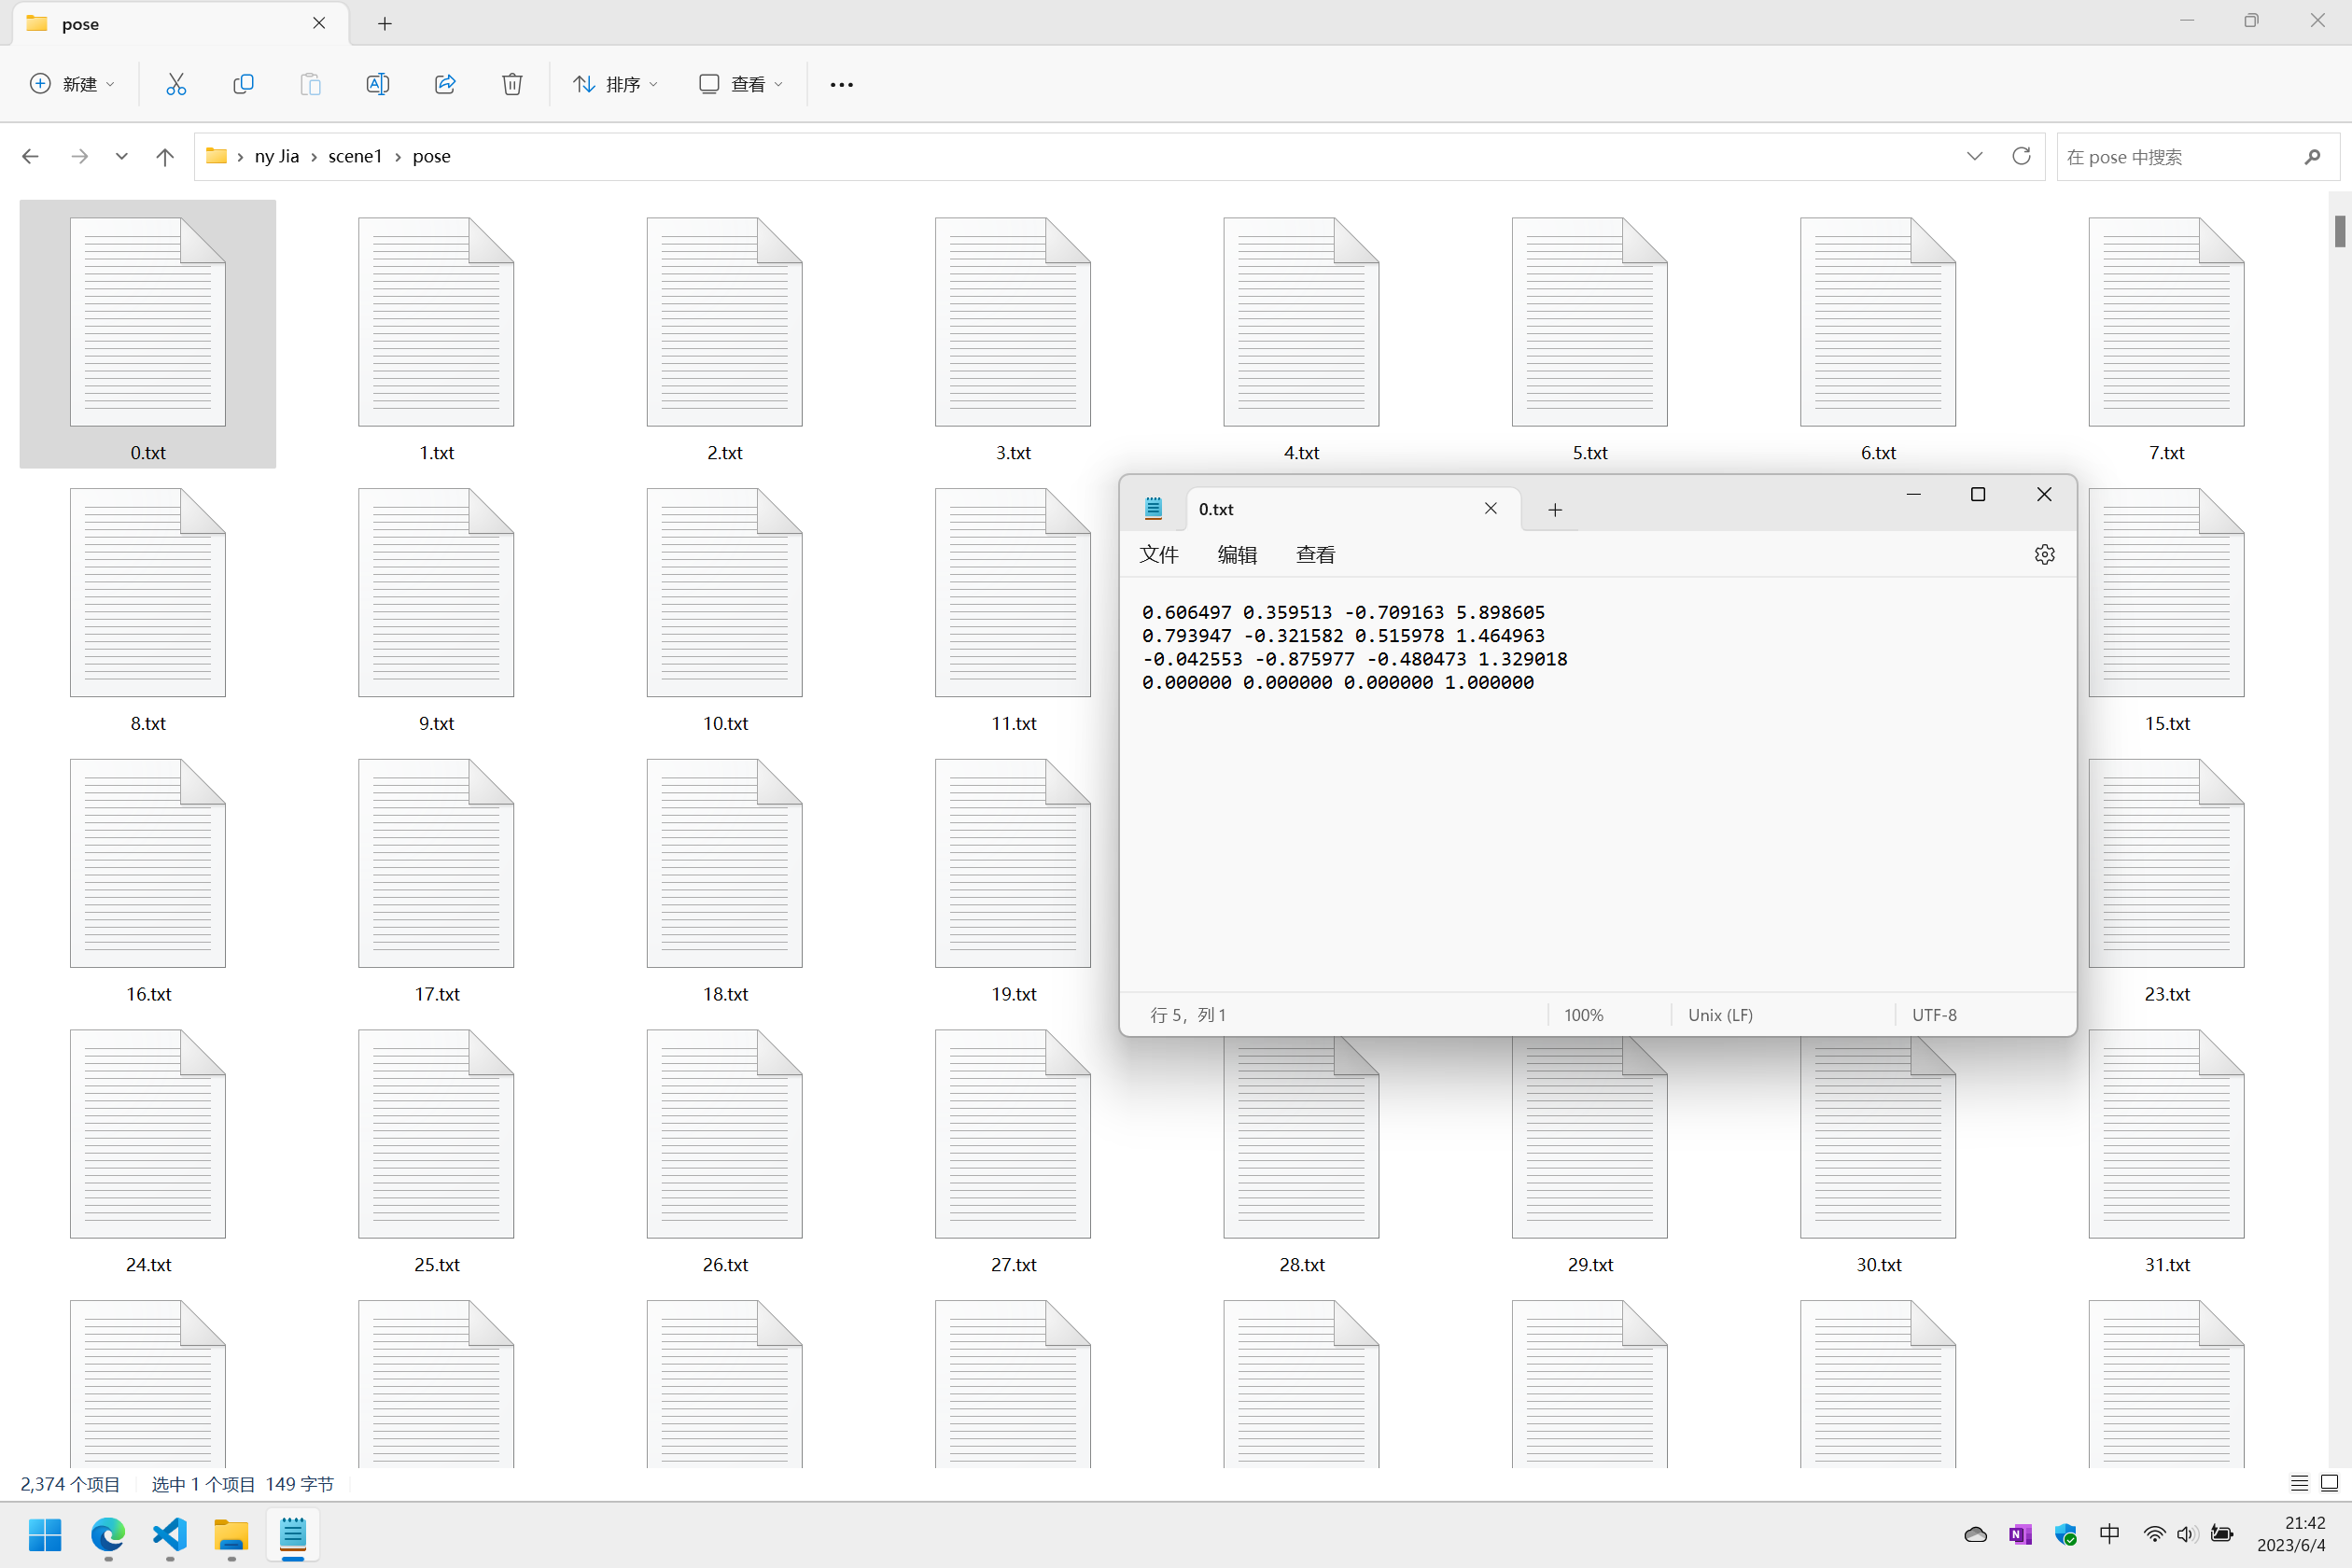
\includegraphics[width=1\textwidth]{figures/scene1_pose.png}
		\caption{位姿估计结果}
		\label{fig:pose_eval}
	\end{minipage}
\end{figure}

\par 图\ref{fig:origin_img}展示了 RGB-D 相机采集的视频流,每帧包括RGB图像和深度图像。其中,RGB图像可以看到环境的颜色和光照等。
\par 图\ref{fig:seg_image}展示了对RGB图像进行语义分割后的图像。每个像素都被赋予了一个语义标签,不同的标签通过不同的颜色表示出来。例如,黄色表示“椅子”,绿色表示“地板”等等。
\par 图\ref{fig:pose_eval}展示了对视频流的每帧图像进行相机位姿估计的结果。每个txt文件中有一个$4 \times 4$的矩阵,即当前帧对应的相机位姿矩阵。

\begin{figure}[htbp]
	\centering
	\subfigure{
		\begin{minipage}[t]{0.84\linewidth}
			\centering
			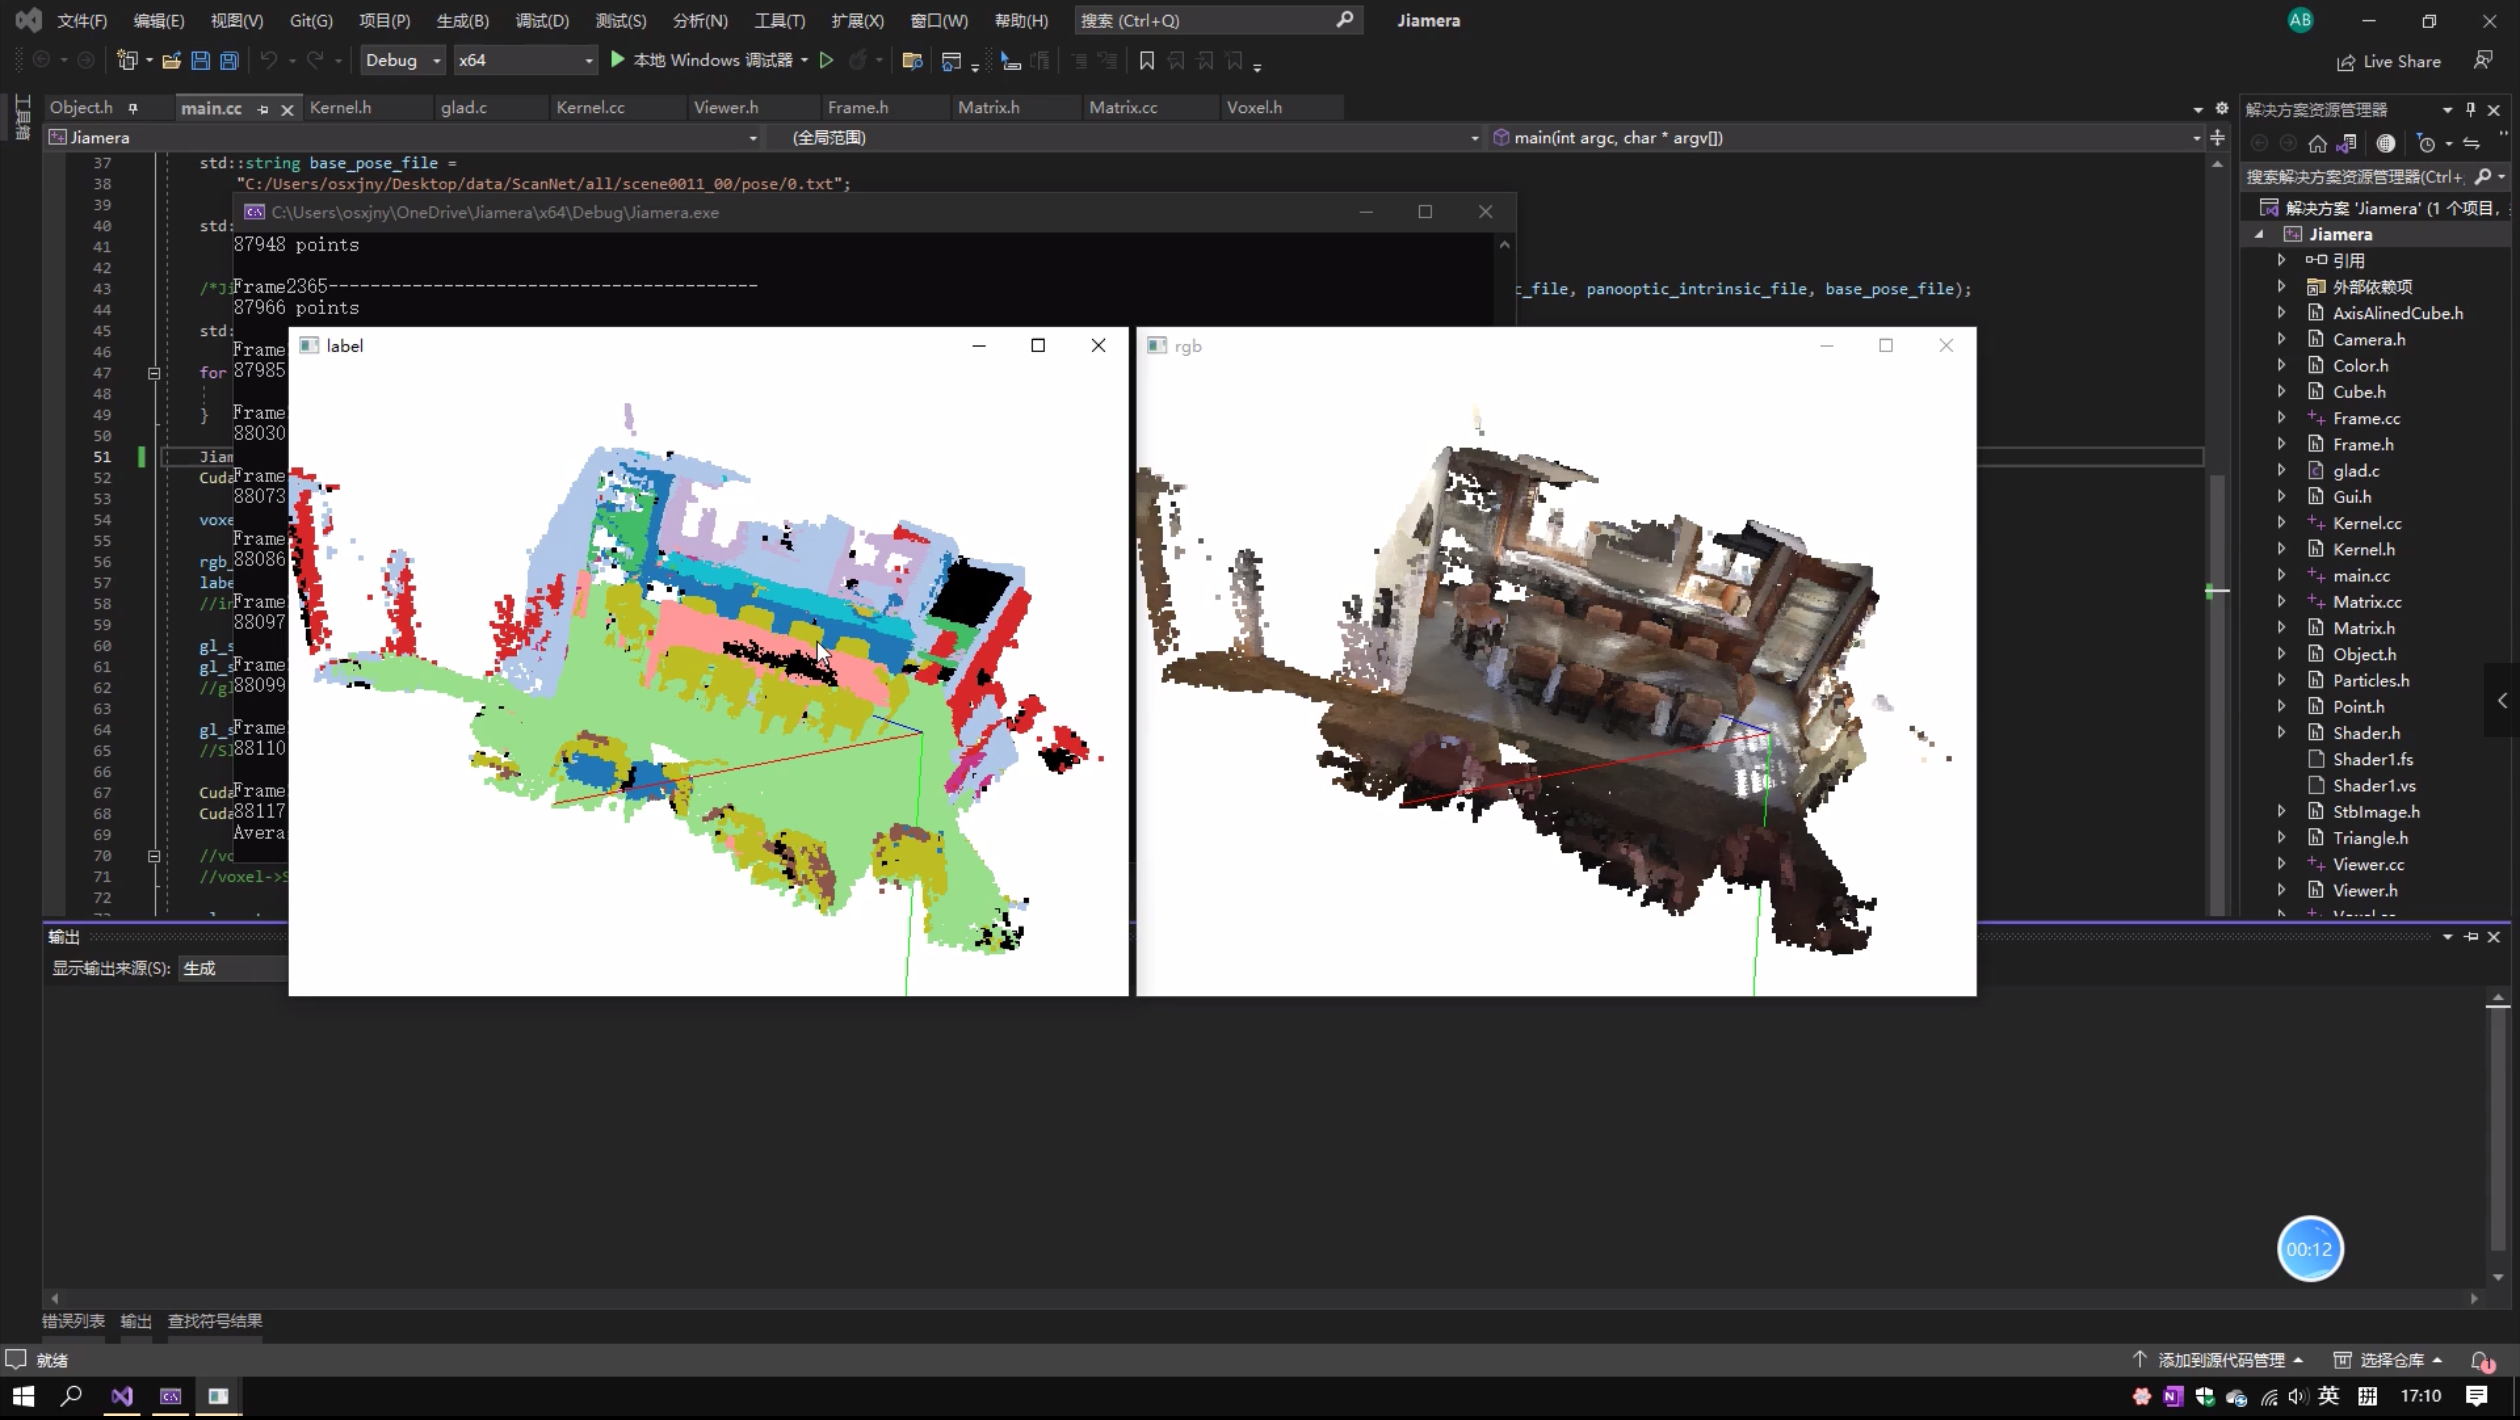
\includegraphics[width=1\textwidth]{figures/test_para/win_all_run.png}
		\end{minipage}
	}
	\caption{在Windows平台运行界面}
	\label{fig:run_result_windows}
\end{figure}

\par 图\ref{fig:run_result_windows}和图\ref{fig:run_result_ubuntu}展示了可视化模块的图形用户界面。这个界面可以清楚地看到物体的形状和位置,包含物体的RGB信息和语义信息。此外,用户可以通过键盘和鼠标输入对动画进行调整和控制,全方位实时观看三维重建的过程。

\begin{figure}[htbp]	
	\centering
	\subfigure[Ubuntu RGB动画]{
		\begin{minipage}[t]{0.48\linewidth}
			\centering
			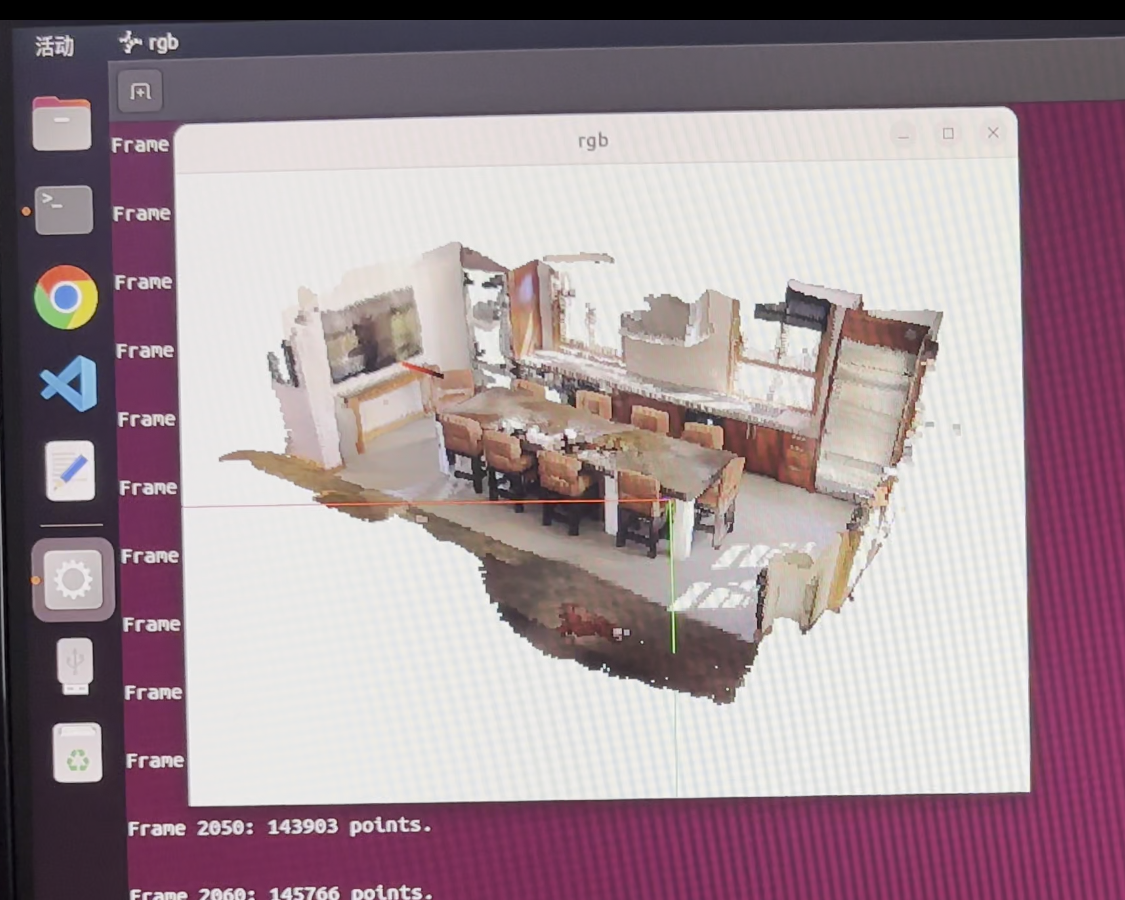
\includegraphics[width=1\textwidth]{figures/test_para/ubuntu_rgb_run.png}
		\end{minipage}
	}
	\subfigure[Ubuntu 语义动画]{
		\begin{minipage}[t]{0.48\linewidth}
			\centering
			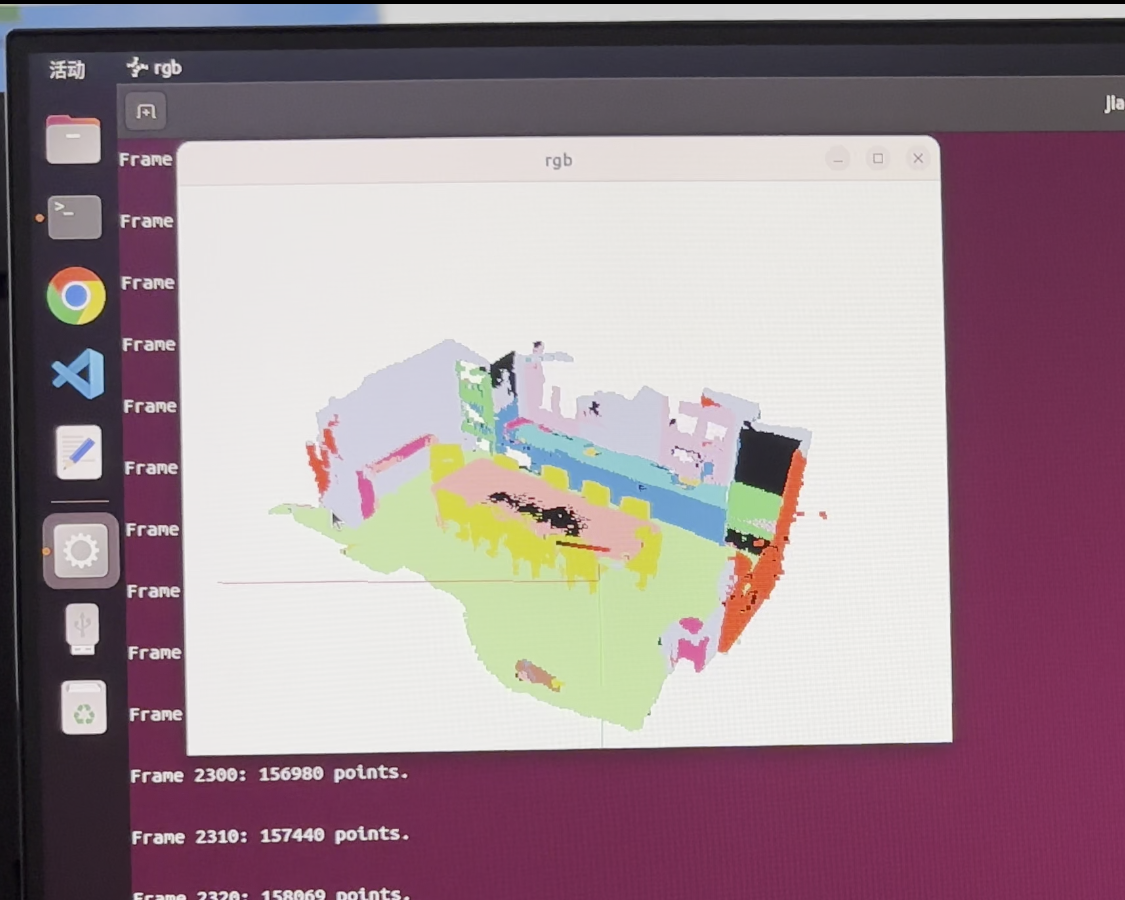
\includegraphics[width=1\textwidth]{figures/test_para/ubuntu_label_run.png}
		\end{minipage}
	}
	\caption{在Ubuntu平台运行界面}
	\label{fig:run_result_ubuntu}
\end{figure}

\par 图\ref{fig:export_result}展示了模型导出的结果。导出模型包括了每个点的三维坐标、RGB信息以及语义信息。

\begin{figure}[htbp]
	\centering
	\subfigure[RGB信息2cm模型]{
		\begin{minipage}[t]{0.48\linewidth}
			\centering
			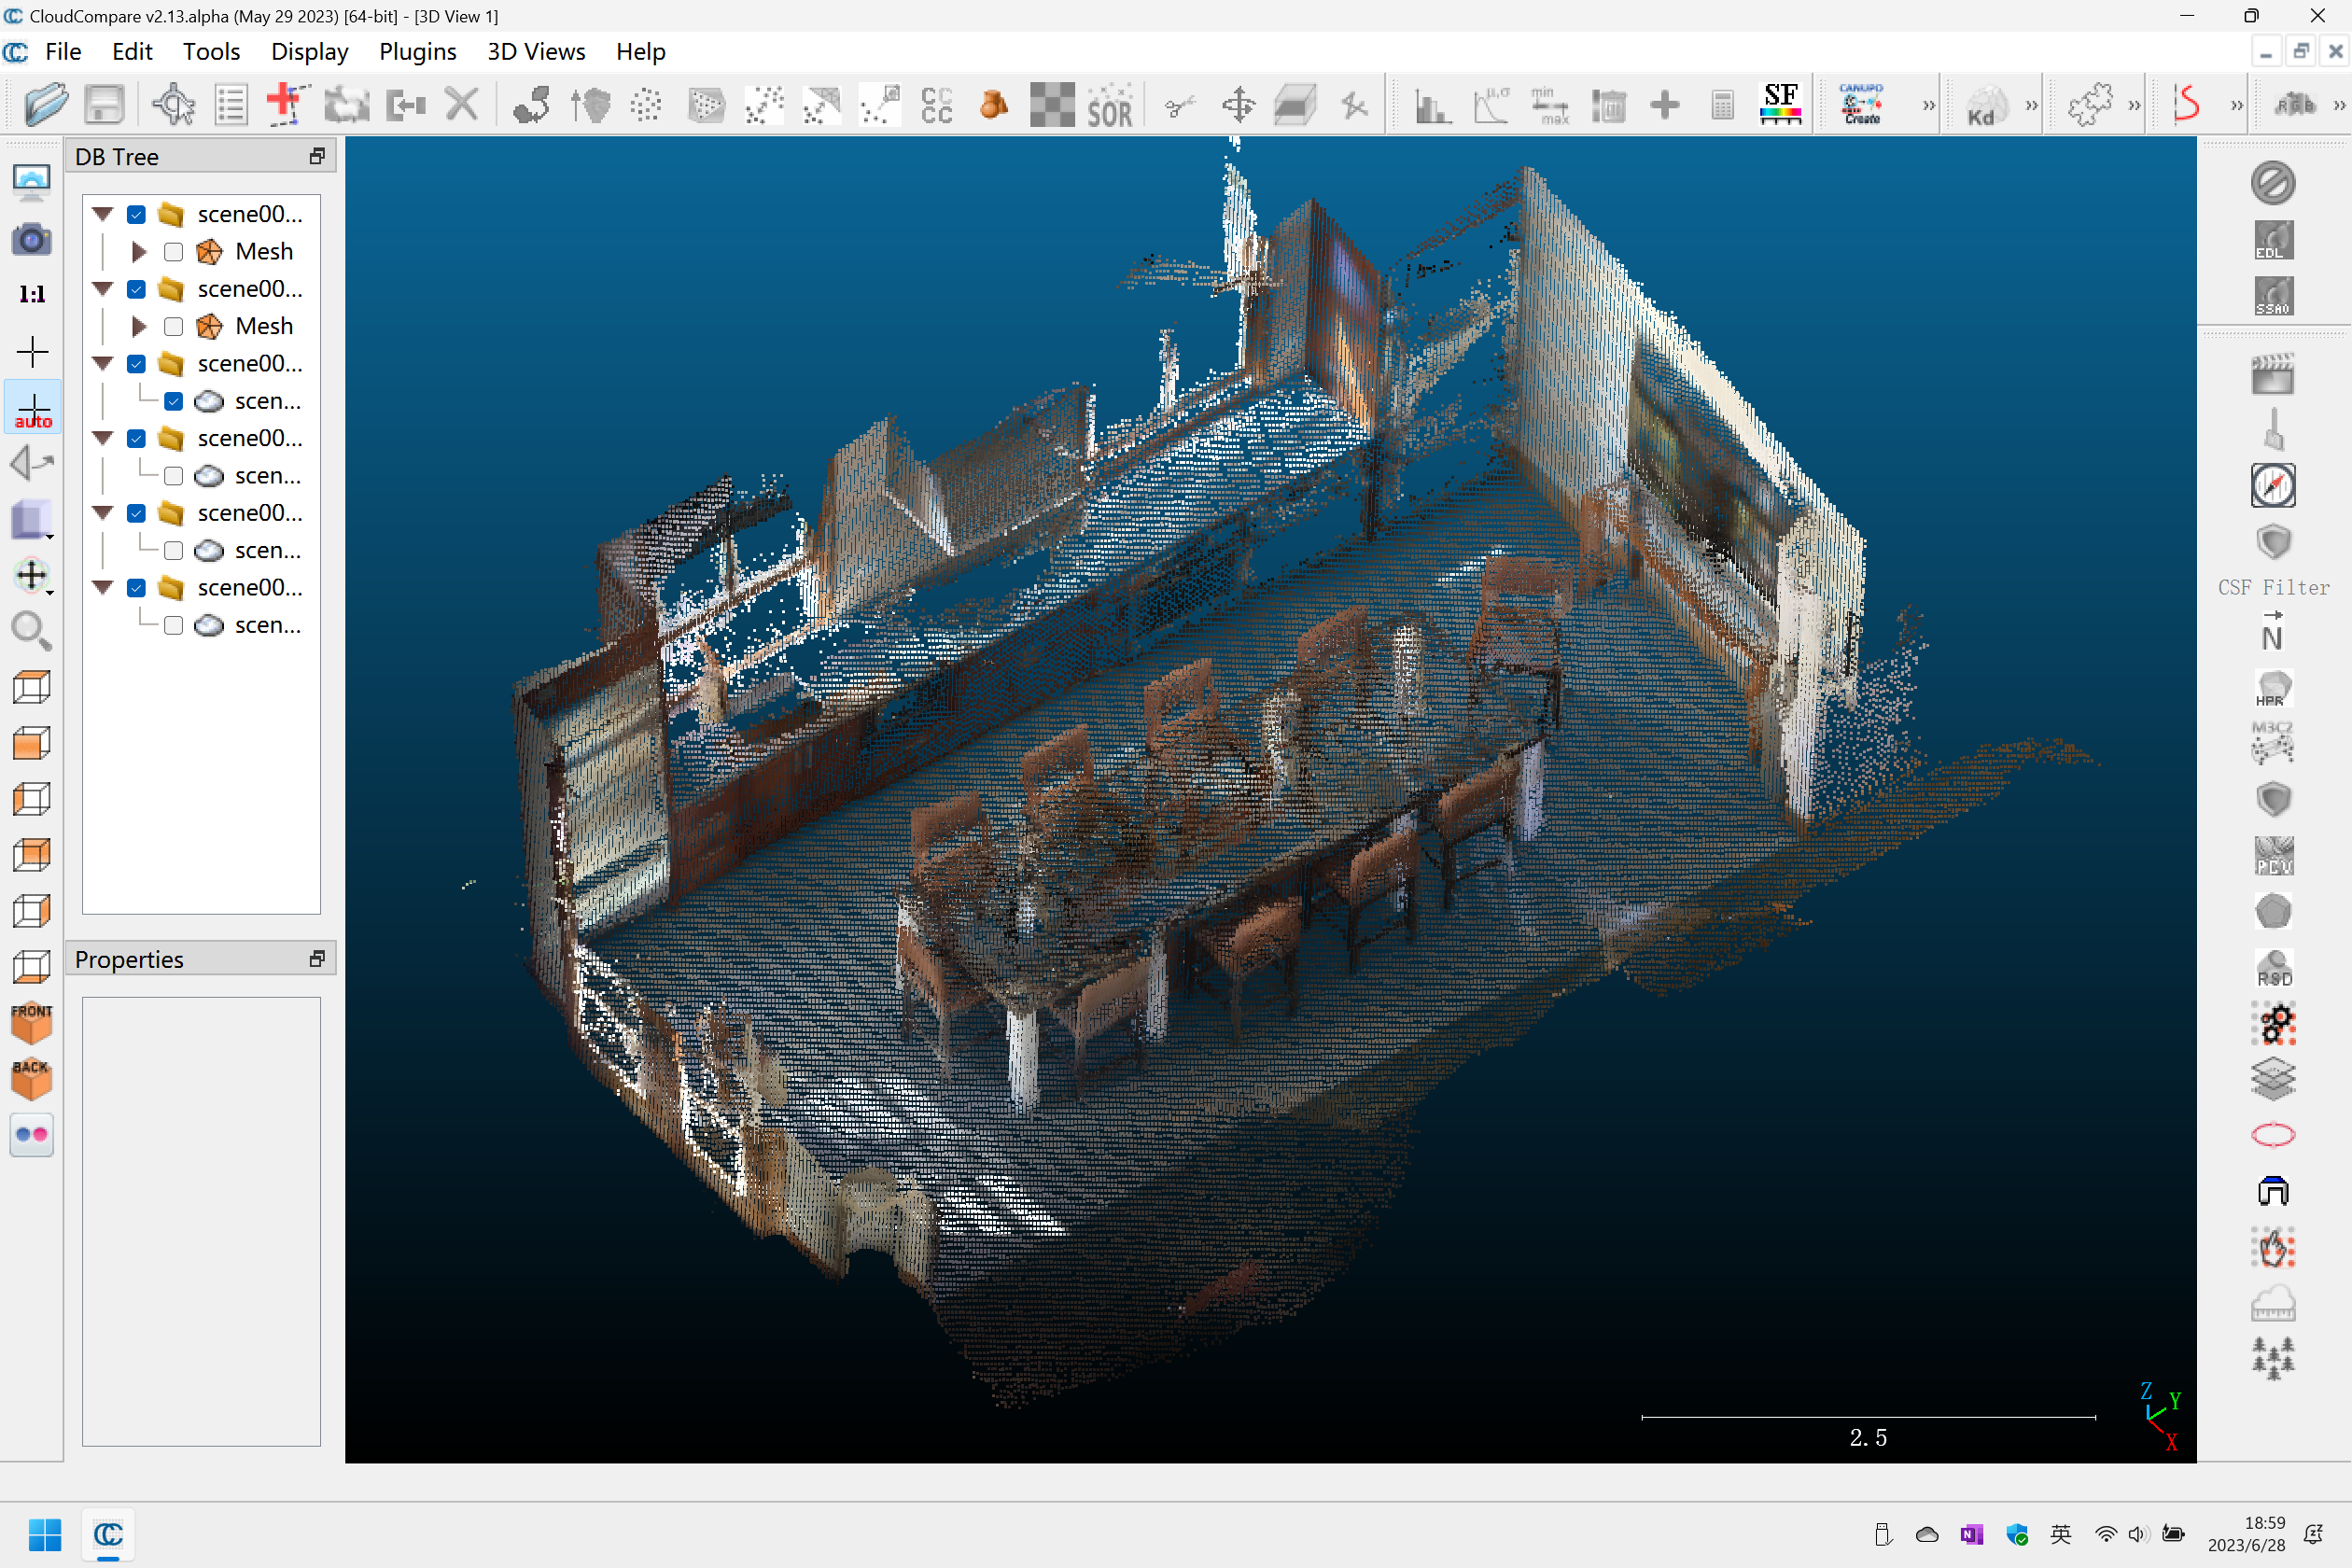
\includegraphics[width=1\textwidth]{figures/result/scene0011_rgb_2cm.png}
		\end{minipage}
	}
	\subfigure[RGB信息5cm模型]{
		\begin{minipage}[t]{0.48\linewidth}
			\centering
			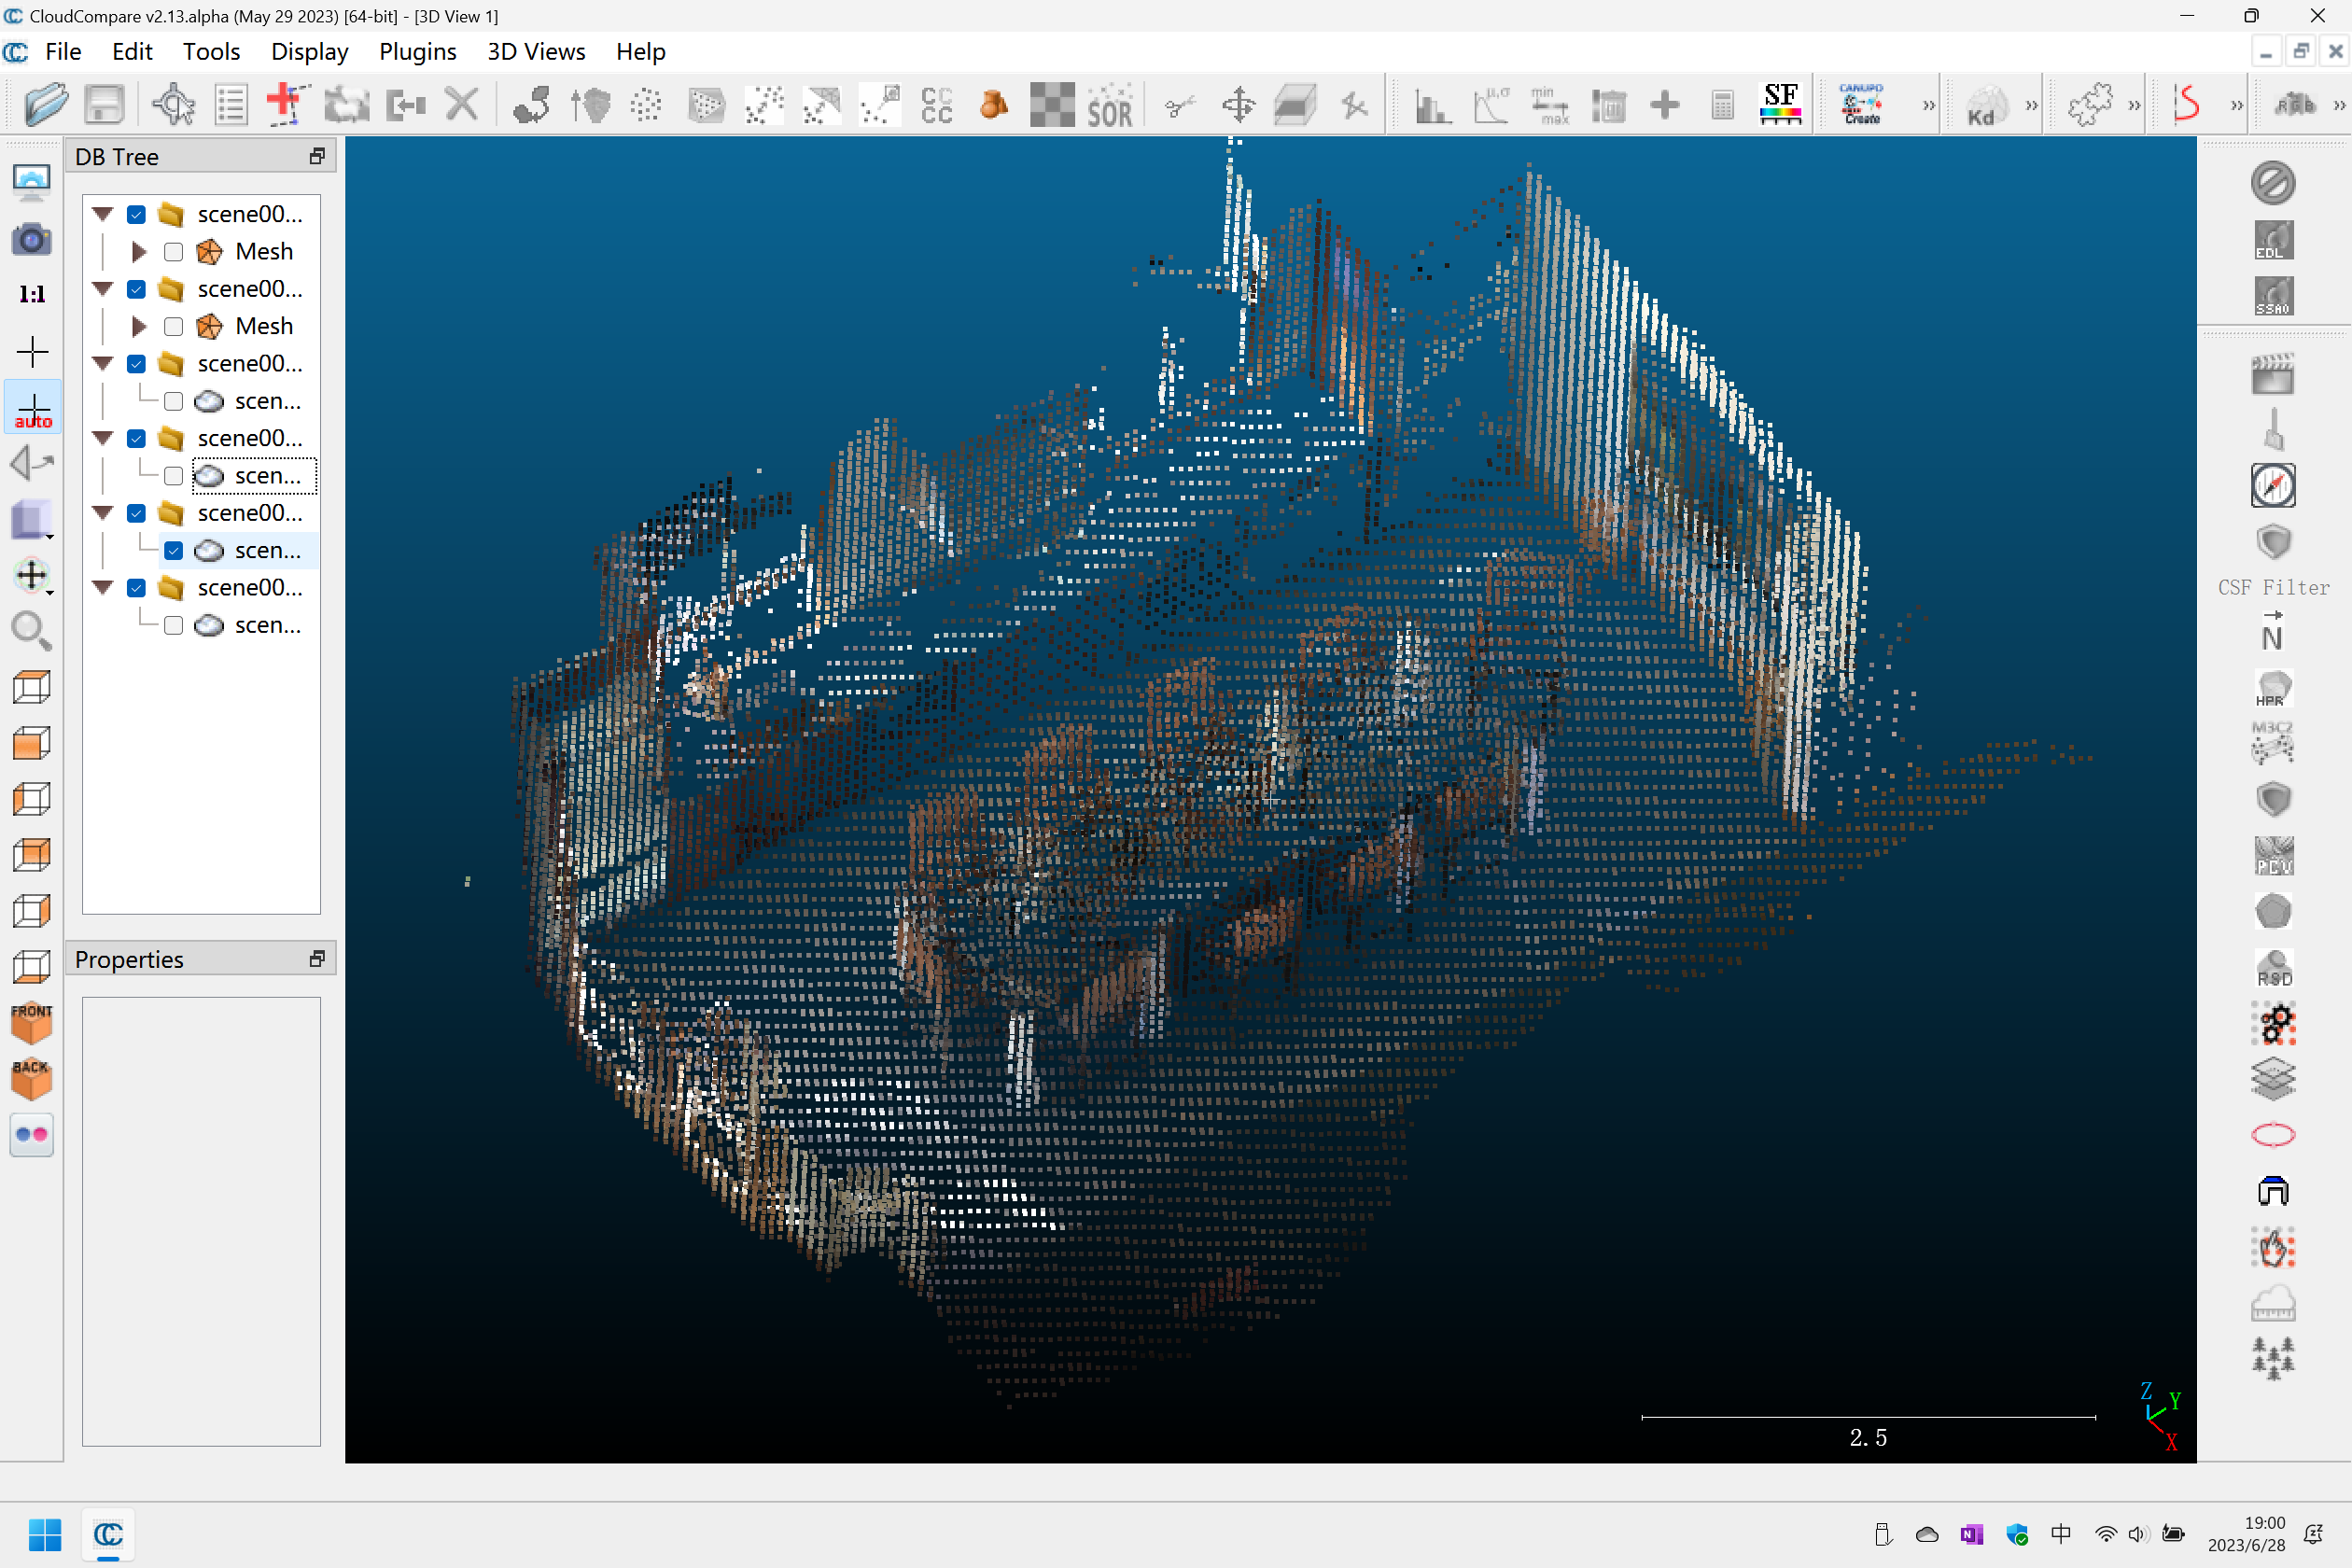
\includegraphics[width=1\textwidth]{figures/result/scene0011_rgb_5cm.png}
		\end{minipage}
	}

	\subfigure[语义信息2cm模型]{
		\begin{minipage}[t]{0.48\linewidth}
			\centering
			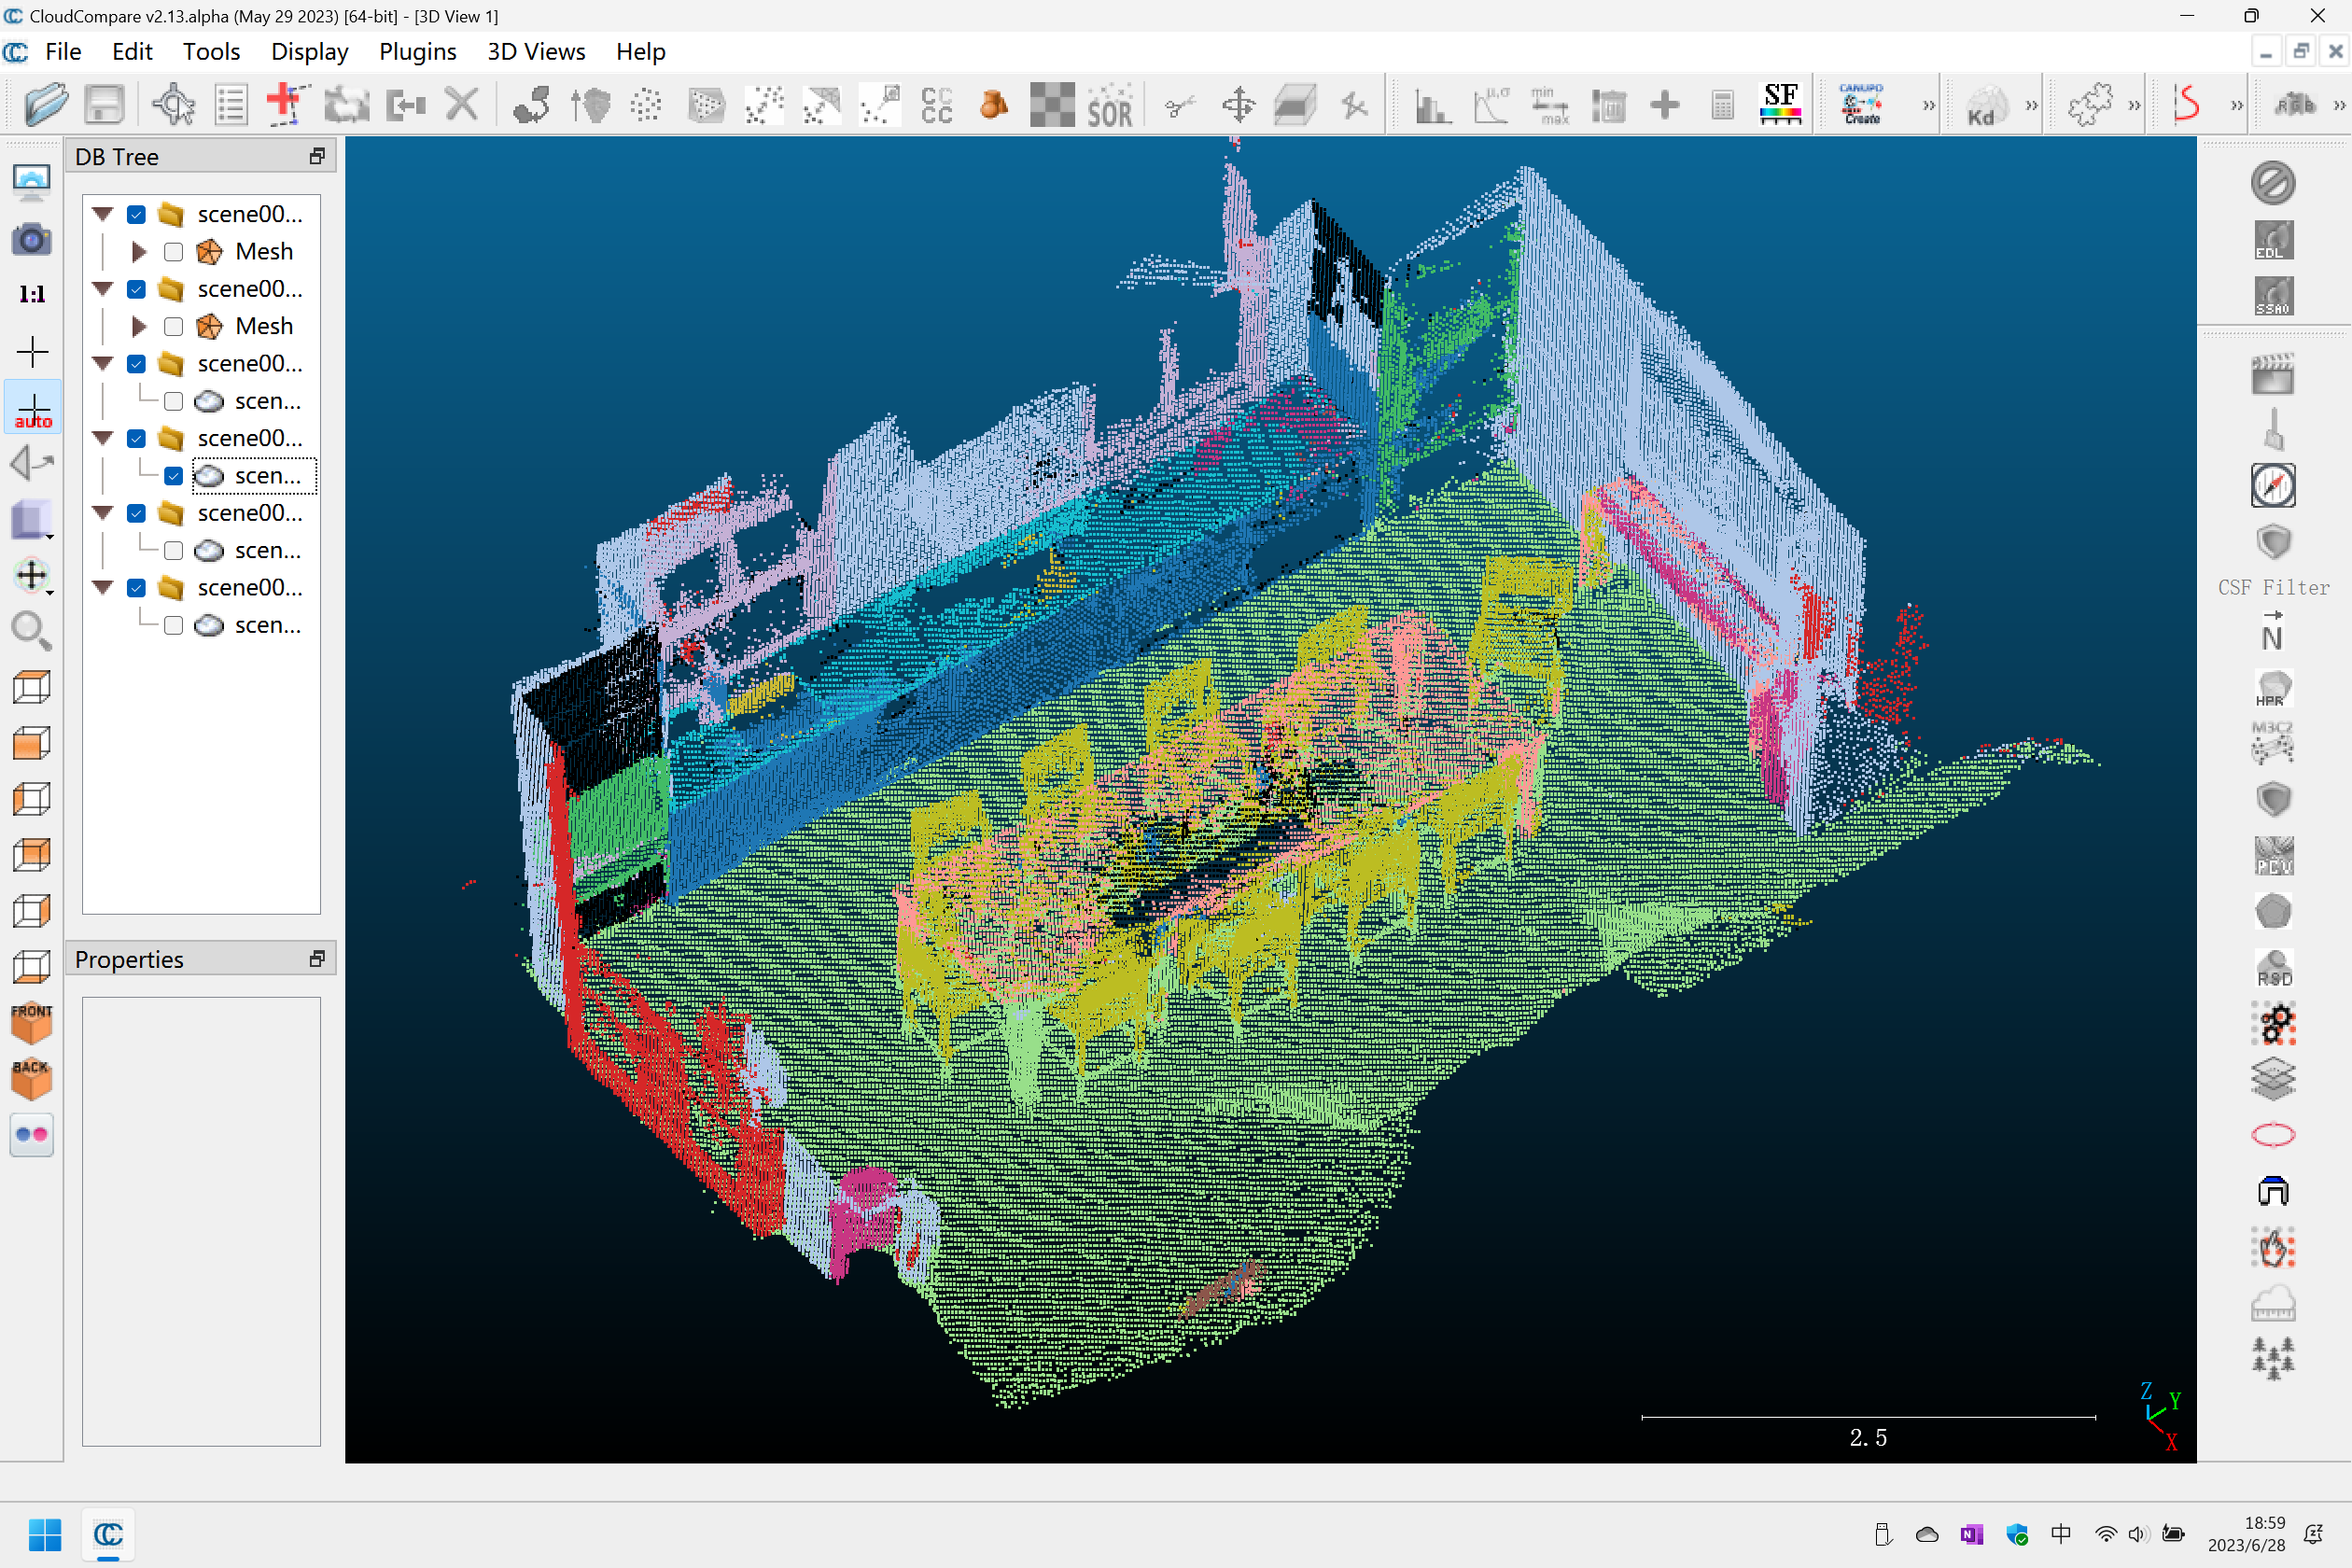
\includegraphics[width=1\textwidth]{figures/result/scene0011_label_2cm.png}
		\end{minipage}
	}
	\subfigure[语义信息5cm模型]{
		\begin{minipage}[t]{0.48\linewidth}
			\centering
			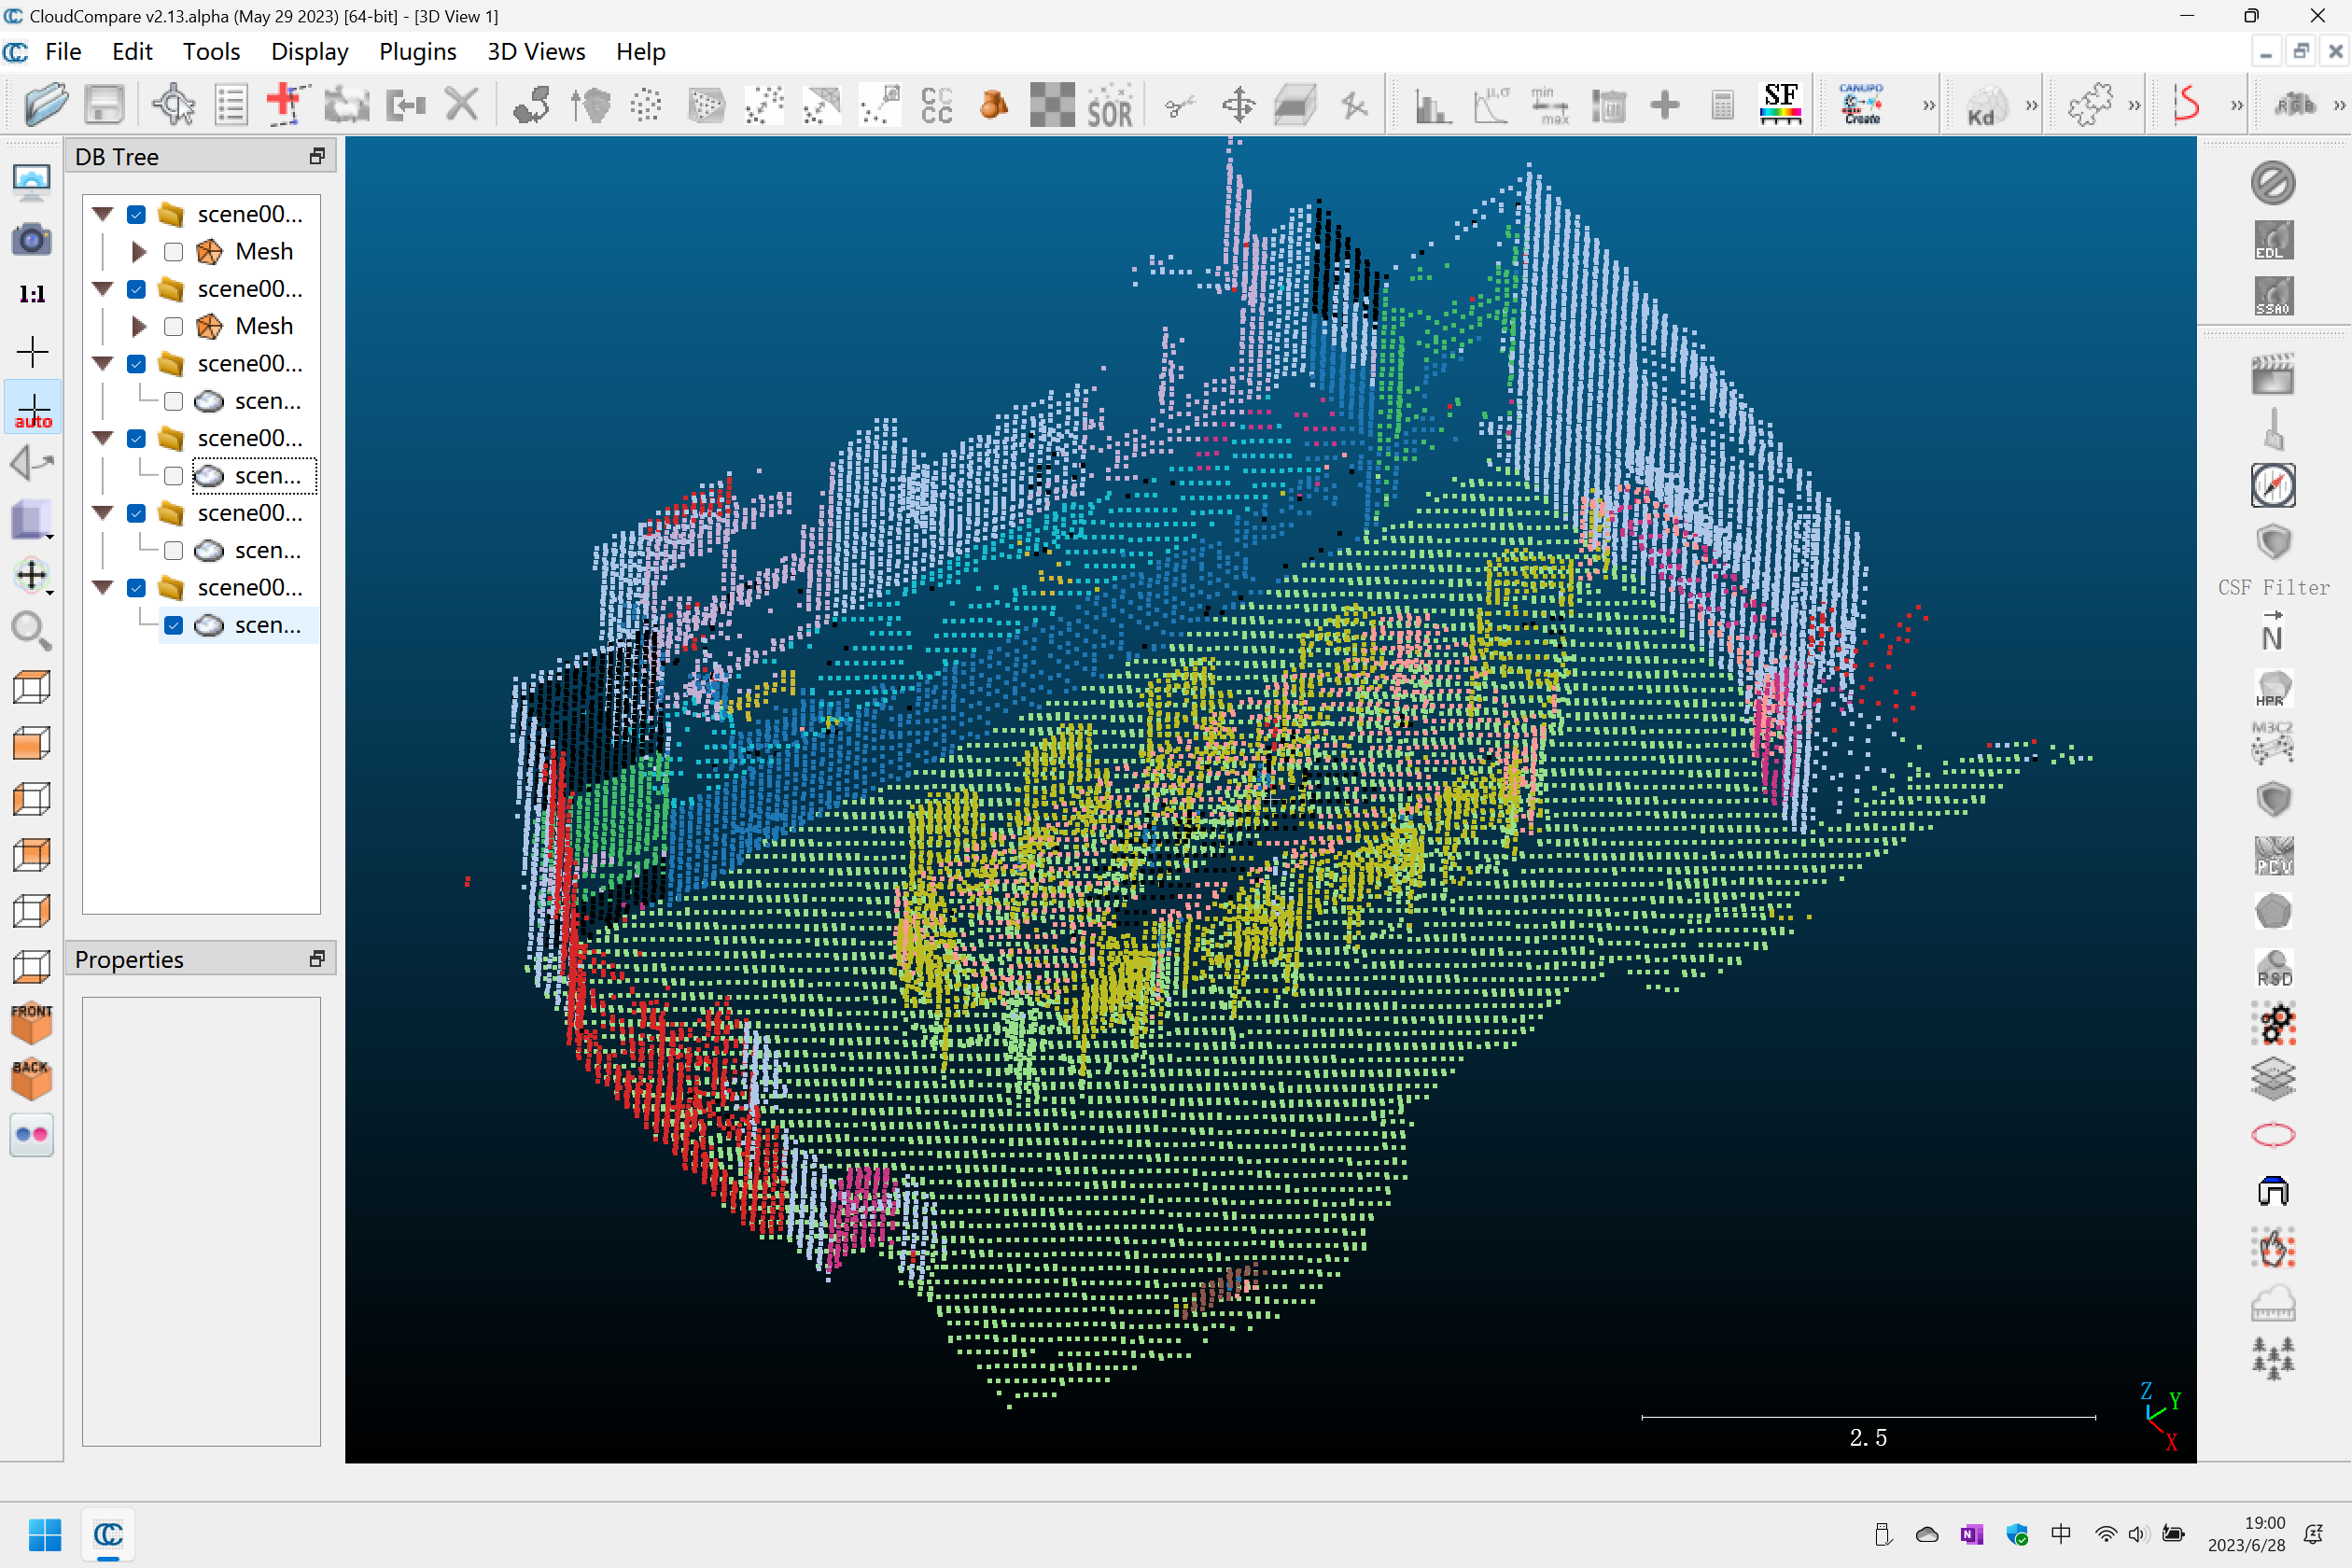
\includegraphics[width=1\textwidth]{figures/result/scene0011_label_5cm.png}
		\end{minipage}
	}
	\caption{模型导出结果}
	\label{fig:export_result}
\end{figure}

\section{本章小结}
\par 本章详细介绍了系统的设计与实现过程。首先,从模块化的角度,对系统进行了分析和设计,详细描述了每个模块的功能和工作流程。其次,明确了开发环境,并以此介绍了本系统采用的开发方法。最后,通过展示系统在运行过程中和运行结果的截图,阐明了系统实现效果的具体情况。